\chapter{RESULTS AND DISCUSSIONS}
\label{chap:Results}

\section{Neural network-based obstacle avoidance for mobile robots}

The results obtained in the experiments show that the neural networks for obstacle avoidance trained entirely with the data obtained in simulation can have good performance in the real world without any additional training with real-world data. In the following subsections, each of the experiment results is reported and discussed.

\subsection{Parameters identification experiment}\label{Sec:ResLabelling}

The first thing to notice in this experiment is that, by using datasets created by using different parameters for the number of LiDAR points and thresholds, the ratio between numbers of positive (no crash) and negative (crash or short period that precedes the crash) training samples is different, although the same raw data are used. That is because, when using lower threshold values, the robot can come closer to the obstacle and for that reason, there are more positive samples than with higher threshold values. Similar reasoning can be applied to the other parameter in question, the number of points needed to classify a sample as negative. Note that positive samples likely won't result in a crash, while negative samples would result in a collision. This parameter also had a significant impact on the imbalance between the positive and negative samples in the dataset since the number of points is a crucial parameter to decide if something is an obstacle or not. The ratios between positive and negative samples as a function of these parameters are shown in \cref{fig:Brojevi}. Finally, please note that data in the figure is for the neural network for moving forward; similar trends emerge for neural networks for going left and right.

\begin{figure}
\centering
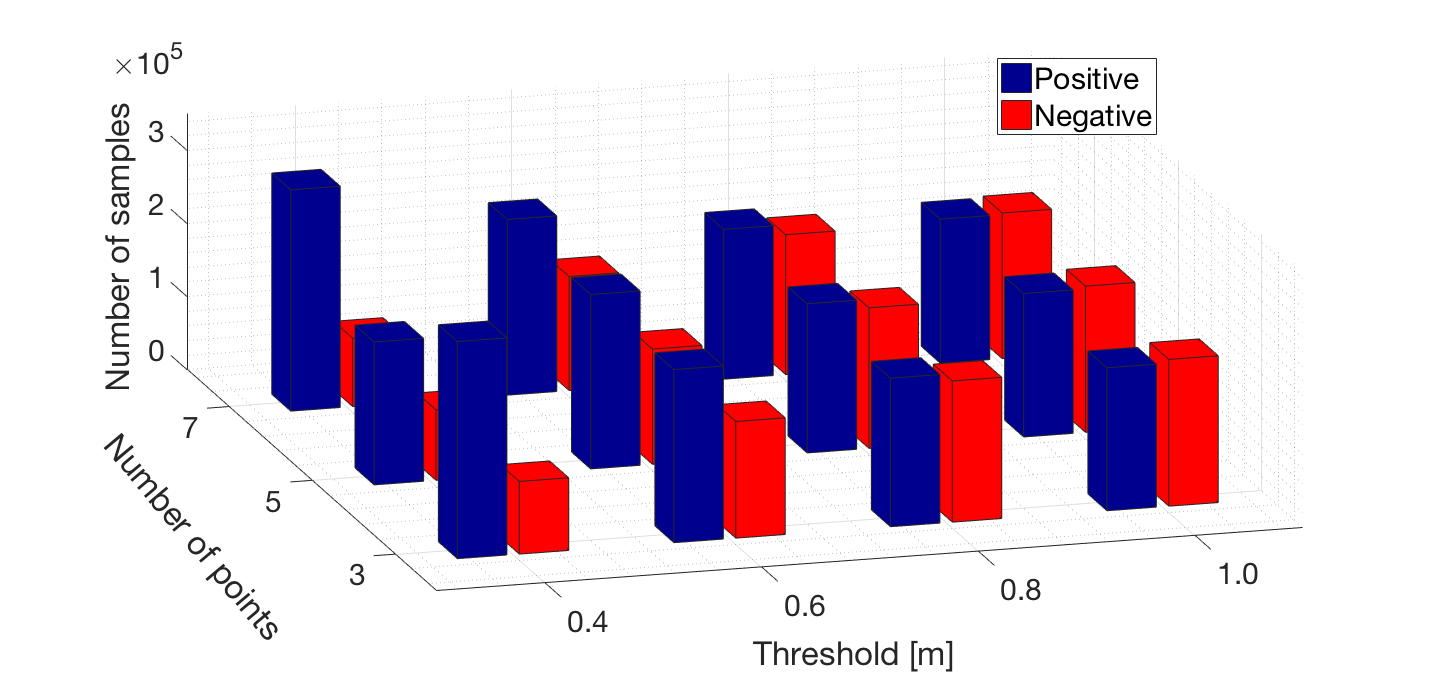
\includegraphics[width=0.9\textwidth]{slike/Fig04_01.png}
\caption{The number of positive and negative samples per dataset}
\label{fig:Brojevi}
\end{figure}

It was also observed that there were more crash events for datasets created with threshold parameter values of 0.4 m and 0.6 m than with other setups. It is likely due to the uneven numbers of positive and negative samples used for the training of neural networks (as per Figure \ref{fig:Brojevi}). These datasets have a significantly higher number of positive samples than negative, which is not the case with setups with threshold parameters equal to 0.8 m and 1 m. This disbalance emphasises the importance of negative samples for learning. It is in line with \cite{Gandhi2017}, and neural networks may need to be fed with more training samples given the current ratio between negative and positive samples to achieve improved performance. The experiment also demonstrated that for neural networks trained with a threshold of  1 m robot executed a significant number of in-place rotations due to the course's narrowness (which was 2.16 m and augmented with additional obstacles). The robot is 0.35 m in diameter, so it needed additional in-place rotations to ``find'' an obstacle-free route.

Out of 60 trials with different neural networks (i.e., neural networks trained with different datasets), in 47 trials, the robot did not complete the course (i.e., get to the other side of the corridor/course), while in the other 13 trials the course was completed. This outcome is not surprising since the robot is not aware of the goal point. It freely roams through the course, going forward when the space in front of it is obstacle-free, and avoiding the obstacle otherwise, which often results in the robot turning away from the course end (which should not be considered as a flaw of the approach, but the limitation of the experimental setup).

\begin{table}[H]
\centering
\caption{The summary of parameter identification experiment results with numbers of completed courses, crash events, loops and local minima per each combination of parameters used.}
\label{Tbl:Stats}
\begin{tabular}{ccccccc}
\toprule
\textbf{Points\tablefootnote{The number of LiDAR points needed to classify a sample as negative}} & \textbf{Threshold} & \textbf{Completed} & \textbf{Crashes\tablefootnote{Total number of crashes}} & \textbf{Thin obs.\tablefootnote{The number of crashes into thin obstacle near course end}} & \textbf{Loop} & \textbf{Local minimum}\\
\midrule
\multirow{4}{*}{3} & 0.4 m & 0 & 5 & 1 & 0 & 0\\
& 0.6 m & 1 & 2 & 1 & 2 & 0\\
& 0.8 m & 0 & 0 & 0 & 5 & 0\\
& 1.0 m & 0 & 2 & 2 & 0 & 3\\
\midrule
\multirow{4}{*}{5} & 0.4 m & 0 & 4 & 0 & 1 & 0\\
& 0.6 m & 1 & 3 & 0 & 1 & 0\\
& 0.8 m & 4 & 1 & 1 & 0 & 0\\
& 1.0 m & 4 & 1 & 1 & 0 & 0\\
\midrule
\multirow{4}{*}{7} & 0.4 m & 1 & 4 & 1 & 0 & 0\\
& 0.6 m & 0 & 4 & 3 & 1 & 0\\
& 0.8 m & 2 & 3 & 3 & 0 & 0\\
& 1.0 m & 0 & 1 & 1 & 0 & 4\\
\bottomrule
\end{tabular}
\end{table}

Table \ref{Tbl:Stats} shows a summary of the conducted experiments. From it, it is evident that setups with 7 LiDAR points needed to classify a sample as negative perform worse than other setups when encountering obstacles with a thin profile, like one right before the course end, as shown in Figure \ref{Fig:LabellingTraj}.
The robot collided with that obstacle significantly more often using this setup than with other setups (eight times vs six times using all other setups combined). Such outcomes are most likely because it does not classify such an obstacle as a negative sample. After all, it usually does not occupy at least 7 points in the LiDAR scan. In addition, it is worth noting that the robot avoided that obstacle several times, so it may be concluded that the angle of approach to it may be critical to its avoidance since when approaching it at different angles results in a different number of LiDAR scan points representing that obstacle, as Figure \ref{Fig:Tocke} demonstrates. Given that, when the robot approaches that obstacle frontally, it ``sees'' only 4 LiDAR points, for the approach at 15$^{\circ}$ 8 points, at 30$^{\circ}$ 10 points and 45$^{\circ}$ 12 points.

\begin{figure}
\centering
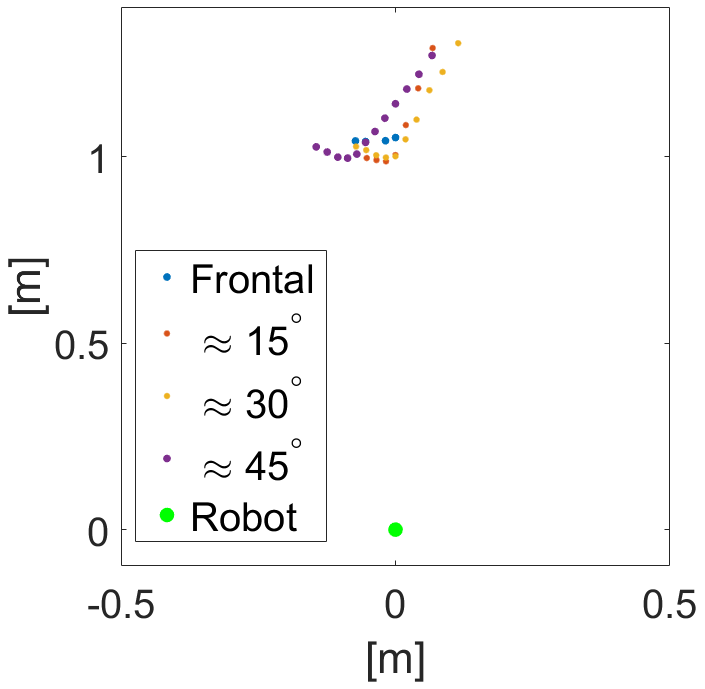
\includegraphics[width=0.5\textwidth]{slike/Fig04_02.png}
\caption{Visualisations of LiDAR scan points when robot approaches thin obstacle from various angles}
\label{Fig:Tocke}
\end{figure}

The timings of experiment trials were recorded and reported for completed course trials, although completion times were not considered a performance metric. The average time and standard deviations per number of points are provided in \cref{Fig:Vrimena}, which demonstrate that the setup with three scan points performs better than others, likely because it can identify more obstacles than other setups and act accordingly, and more identified obstacles might also be a reason why the number of completed courses is so low with that setup compared to others. The setup with seven scan points performs slightly better than the one with five scan points. However, the course was completed only three times, compared to the setup with five scan points completed nine times. Thus, it needs additional testing trials to obtain more general results and draw definite conclusions (based on statistical testing).

\begin{figure}
\centering
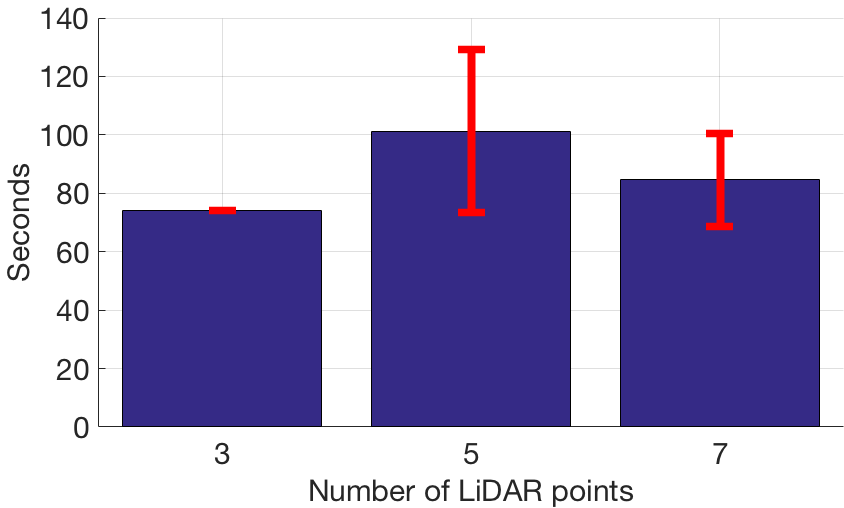
\includegraphics[width=0.5\textwidth]{slike/Fig04_03.png}
\caption{Time analysis of completed course trials}
\label{Fig:Vrimena}
\end{figure}

In some trials, the robot got stuck at local minima. It is noticeable that it only happened with setups that avoid obstacles at a 1 m threshold. Such an outcome is likely due to the narrowness of the experimental course because, at some points in the course, it is impossible to go forward given the sensor readings, so the robot keeps executing in-place rotation to the left and right interchangeably. This issue was resolved in the experiments that followed so that the robot applied a small forward velocity to break out the deadlock.

Results also demonstrated that setups that need 3 LiDAR points (or to some extent also 5 LiDAR points) to classify a sample as negative were too sensitive when using lower threshold values (0.4 m and 0.6 m), since the robot crashed into other obstacles (besides a thin obstacle near the course end) more often than other setups. The crashes might as well be due to the significantly higher number of positive samples than negative samples for training the neural networks for obstacle avoidance.

Examples of the robot trajectories obtained during the experiment are shown in Figure \ref{Fig:LabellingTraj}. Note that the trajectories were captured using AMCL \cite{Fox1997,Thrun2006} which introduces some additional positioning errors. Thus, sometimes in the image, it may seem that there is no crash (when there is, as in Figure \ref{Fig:LabellingTrajb}) or vice versa, that the robot passes ``through'' obstacle (when it passes very close to the obstacle, as in Figure \ref{Fig:LabellingTrajc}).

\begin{figure}
\centering
\subfloat[The trajectory of the completed course \label{Fig:LabellingTraja}]{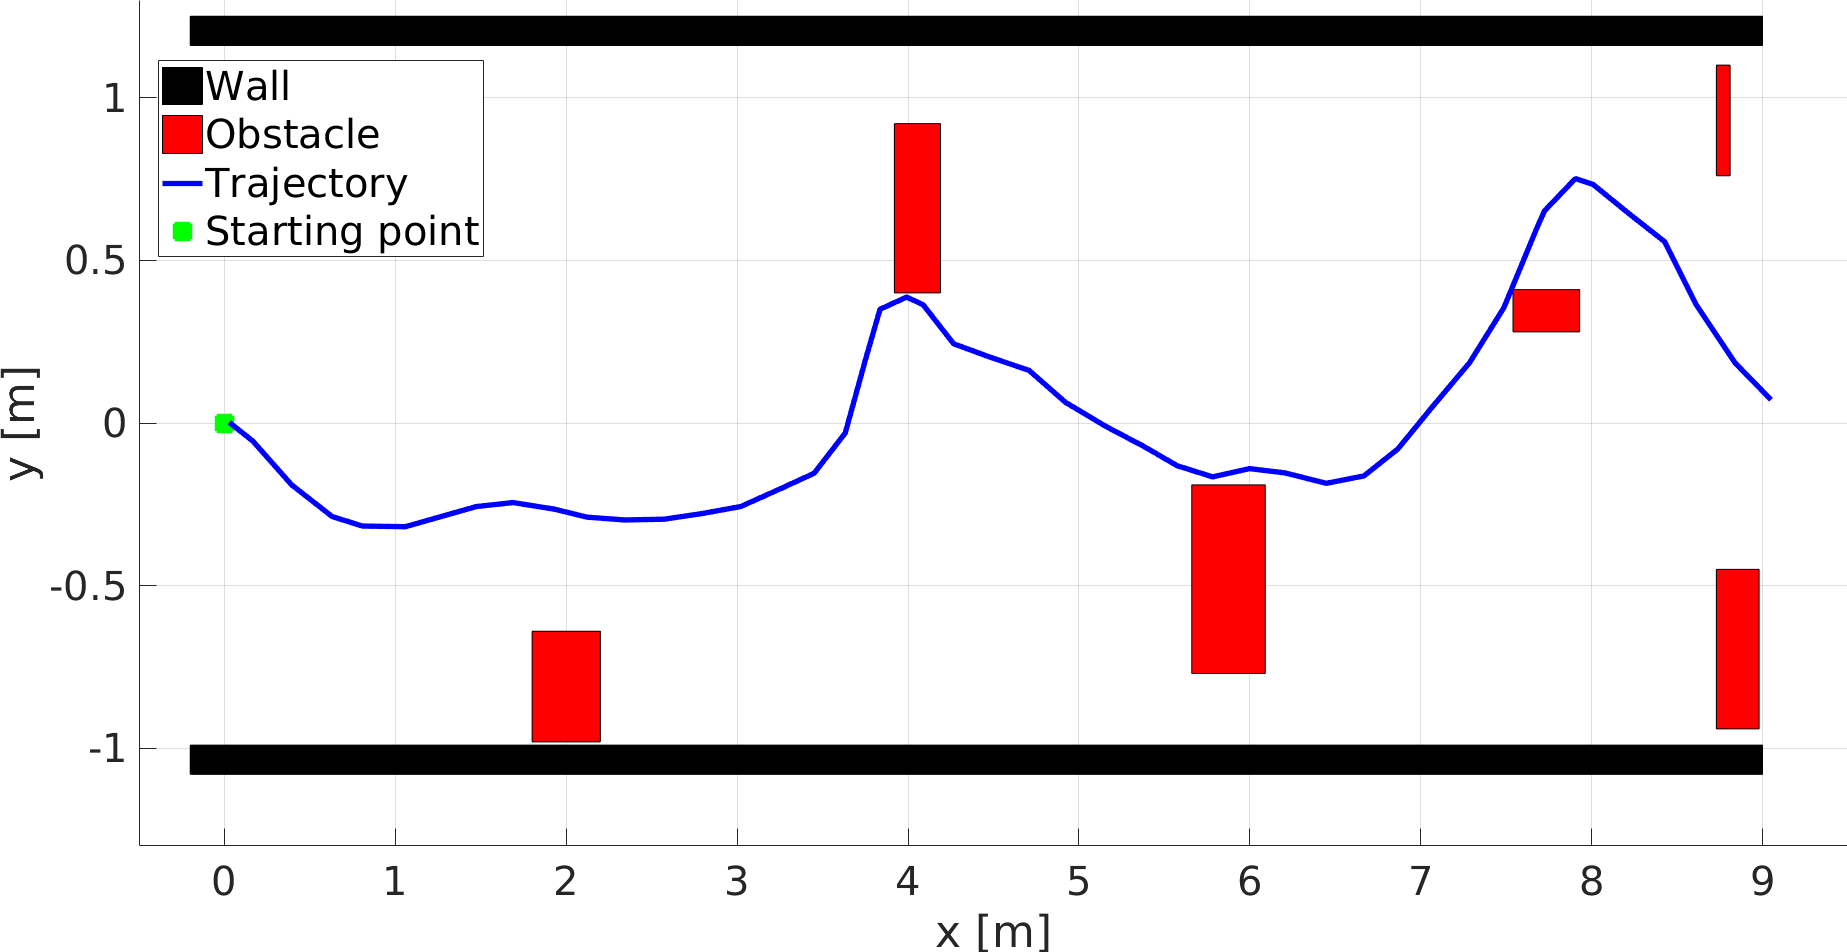
\includegraphics[width=0.495\textwidth]{slike/Fig04_04a.png}}
\hfill
\subfloat[The trajectory of a course that resulted in a crash\label{Fig:LabellingTrajb}]{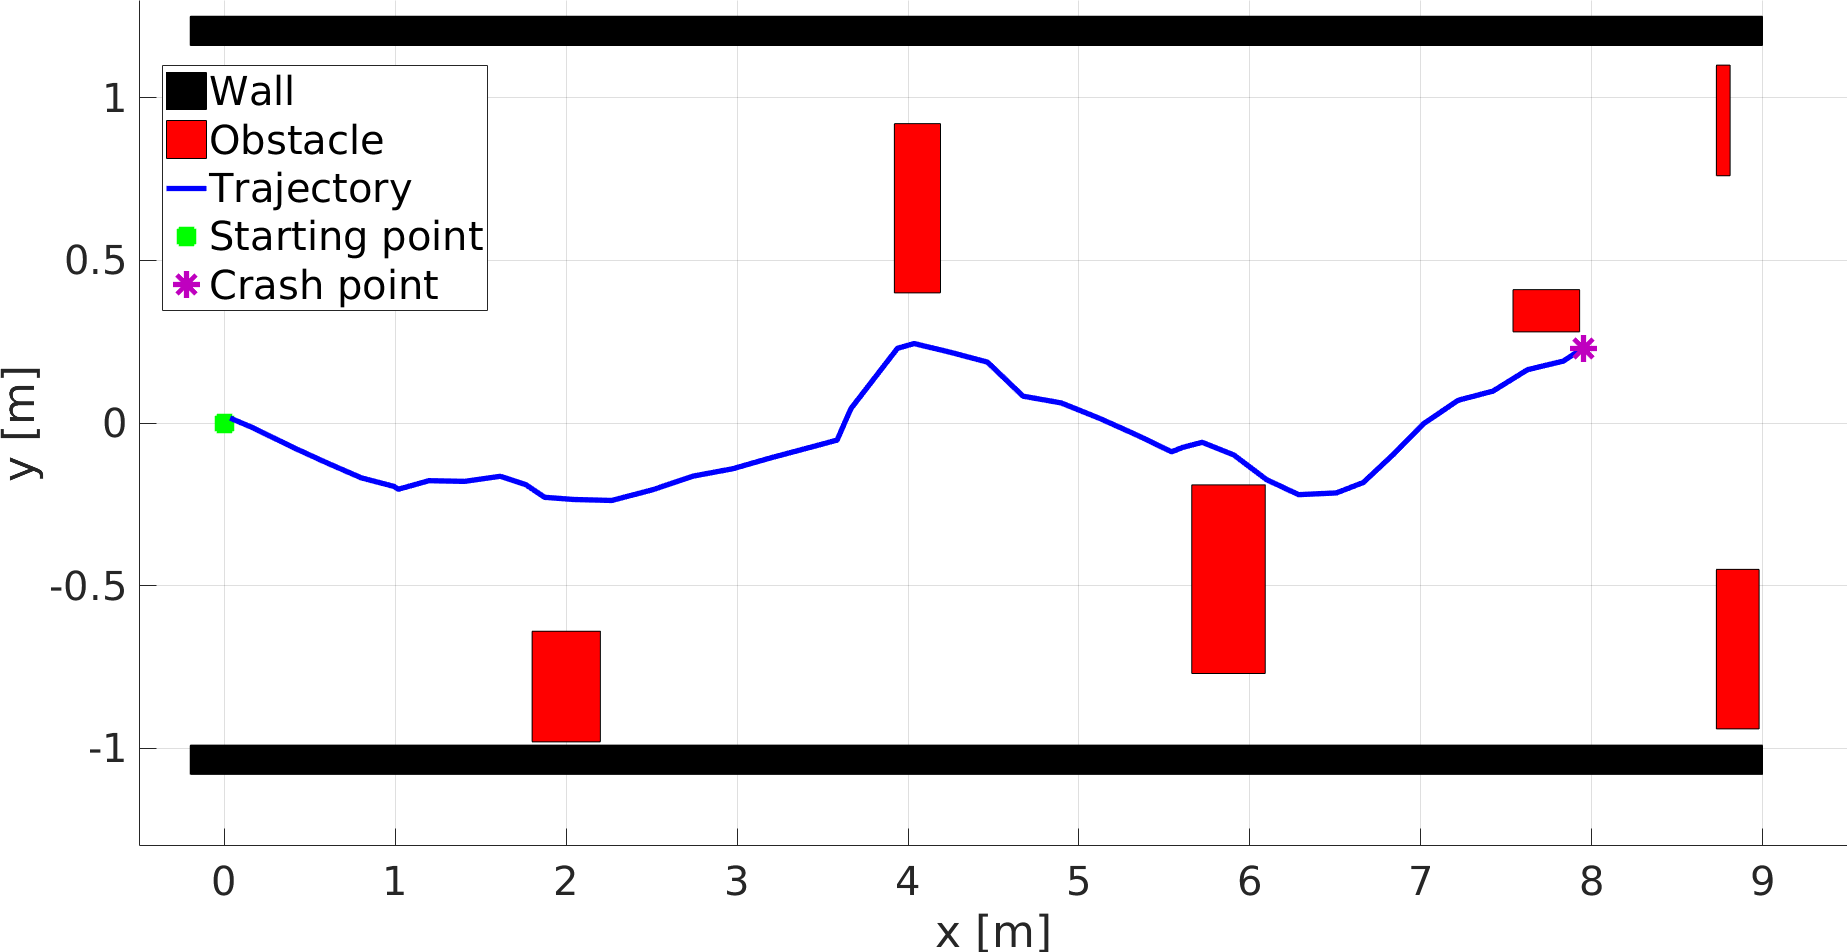
\includegraphics[width=0.495\textwidth]{slike/Fig04_04b.png}}
\vfill
\subfloat[The trajectory of a course that resulted in a loop \label{Fig:LabellingTrajc}]{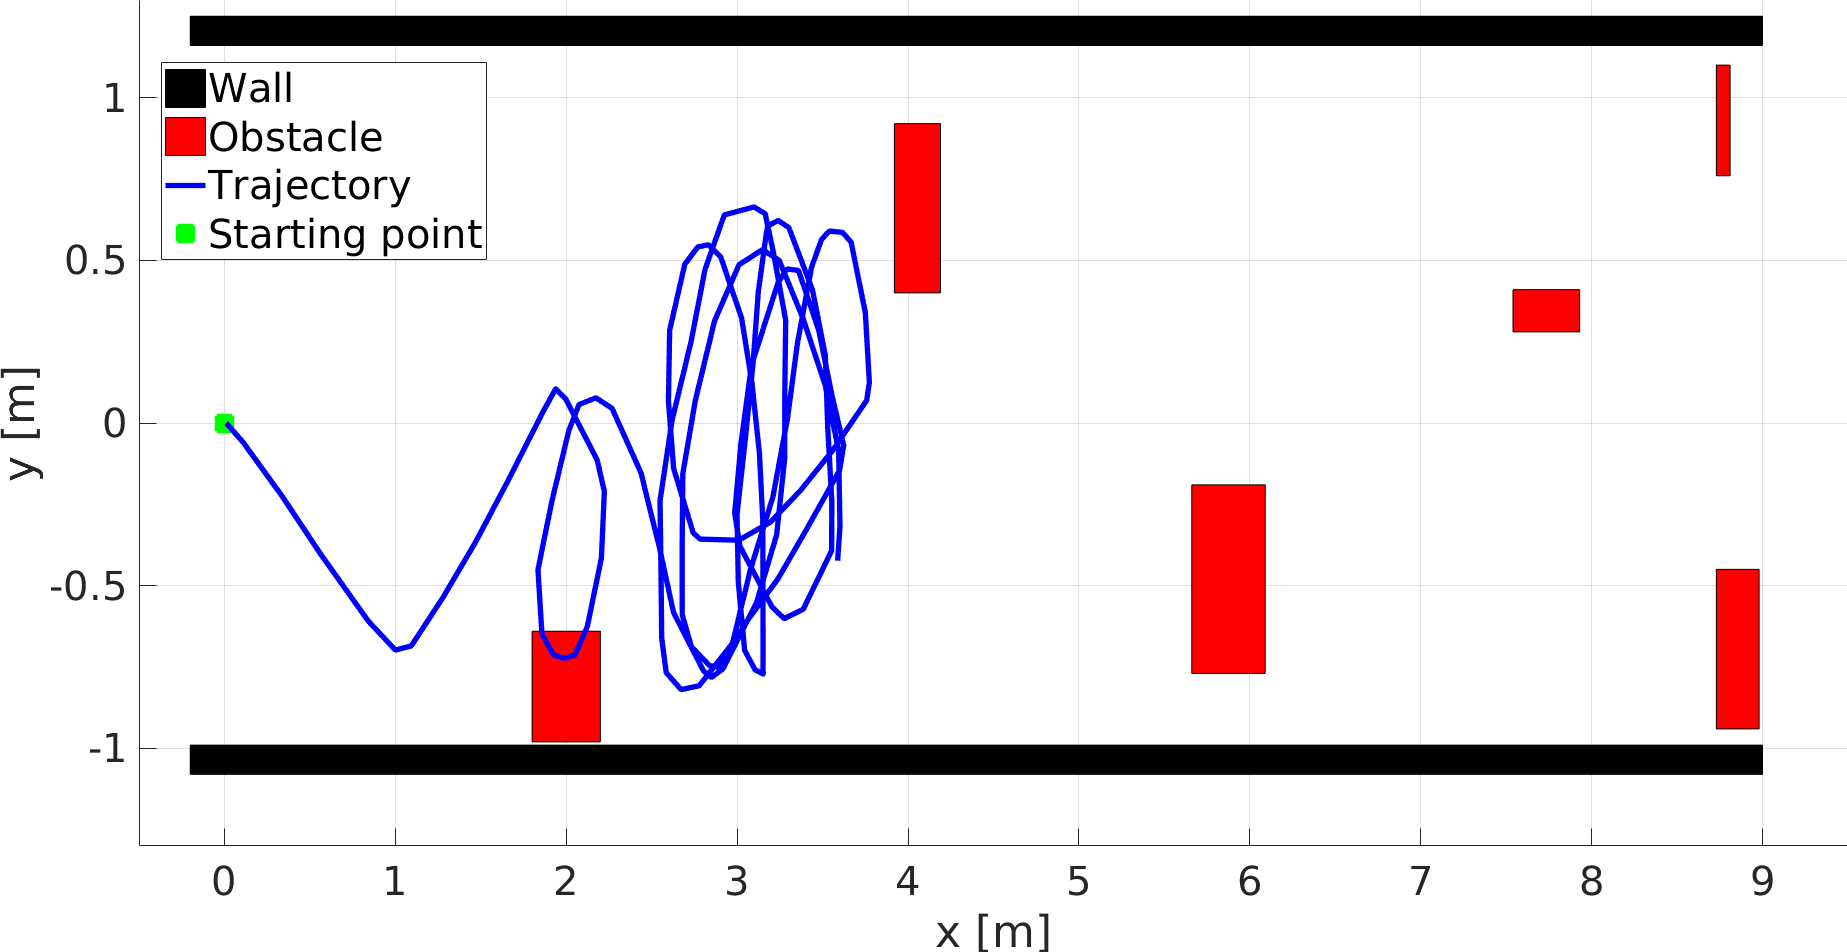
\includegraphics[width=0.495\textwidth]{slike/Fig04_04c.png}}
\hfill
\subfloat[The trajectory of a course in which the robot got stuck at local minimum \label{Fig:LabellingTrajd}]{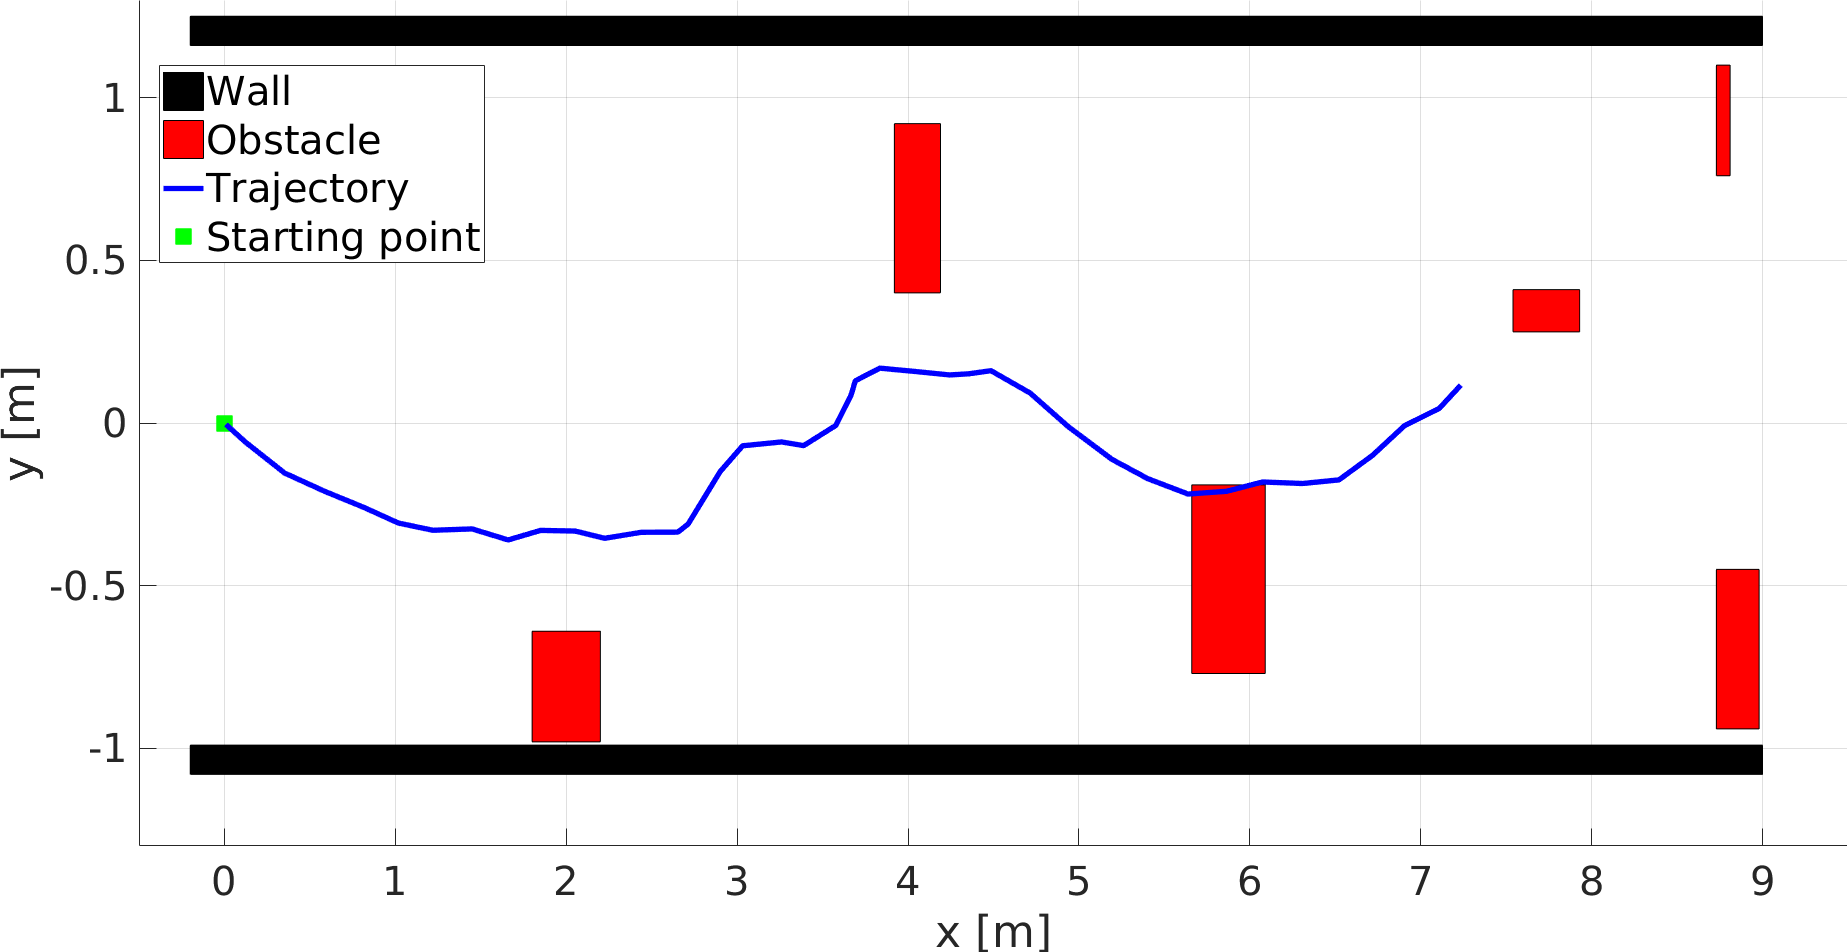
\includegraphics[width=0.495\textwidth]{slike/Fig04_04d.png}}

\caption{Examples of robot trajectories during the arameters identification experiment}
\label{Fig:LabellingTraj}
\end{figure}

Based on the obtained results in the experiment, it was decided to use datasets labelled with a threshold of 1 m and 5 LiDAR scan points for the experiments that followed, both in simulation (\cref{sec:SimulationRes}) and in the real world (\cref{sec:RealRes}).

\subsection{Simulation experiments}
\label{sec:SimulationRes}

In all 20 test runs of the first experiment in simulation, the run was terminated after 10 minutes without a crash. That summed up to a total of 200 minutes of driving without a crash in an environment cluttered with obstacles. These results demonstrated appropriate behaviour in simulation, which motivated us to further test the approach on the real robot. Examples of trajectories obtained during testing in the simulation are shown in Figure \ref{fig:Fig06}. However, it should be noted that if a more dense obstacle configuration was used, crashes might have occurred, but we believe that the used obstacle configuration (remember the size of the whole perimeter is 12.5 m $\times$ 12.5 m) is a good representation of a general office-type environment.

\begin{figure}
    \centering
    \subfloat{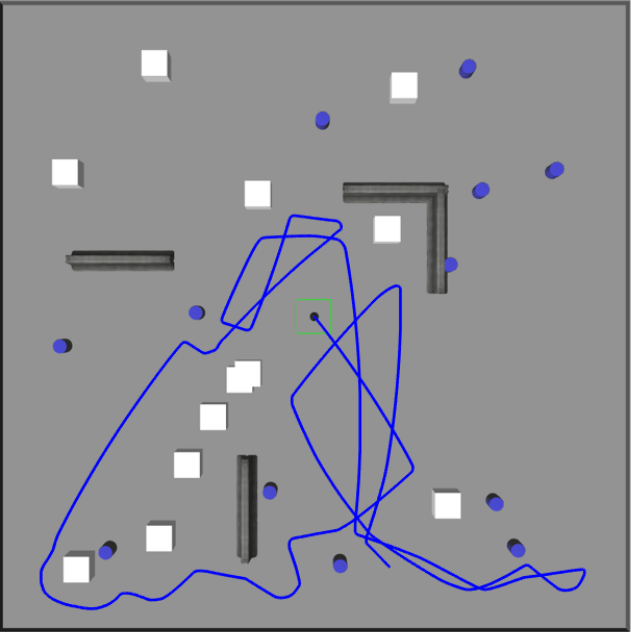
\includegraphics[width=0.495\textwidth]{slike/Fig04_05a.png}}
    \hfill
    \subfloat{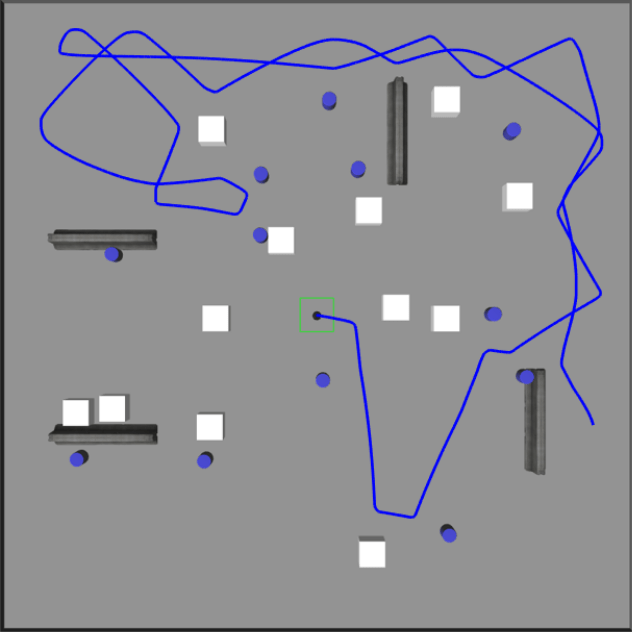
\includegraphics[width=0.495\textwidth]{slike/Fig04_05b.png}}
    \caption{Example trajectories obtained while testing the proposed obstacle avoidance method in simulation.}
    \label{fig:Fig06}
\end{figure}

In the other simulation experiment, which contained a single moving obstacle in a small area, it was observed that the robot had no problem avoiding the moving obstacle if the obstacle velocity was small (0.1 m/s and 0.2 m/s, roughly less than robot velocity). However, crashes occurred with higher obstacle velocities (6 crashes with 0.4 m/s obstacle velocity, and with 0.8 m/s obstacle velocity, the robot could not get past the moving obstacle at any time). While interpreting these results, please keep in mind that the robot velocity was constant (0.2 m/s) and that neural networks controlling the robot were trained without moving obstacles in the scene, and that possibly improved performance could be achieved if moving obstacles are appropriately included in the training set. 

\subsection{Real-world experiments}
\label{sec:RealRes}

In real-world experiments, the first thing that was assessed was the computational speed of the proposed algorithm (mean values for 500 LiDAR scan cycles are reported; of note is that the median values were smaller than the average values in all cases). Each neural network (right, left, forward) took 0.773 ms to produce an output, while the preprocessing of raw LiDAR data (mainly separation to appropriate parts and formatting) took another 0.144 ms. The postprocessing (generation of velocity commands for the mobile robot) took an additional 0.237 ms. Thus, on average, the algorithm took 1.554 ms to produce a velocity command to the robot based on its input. This computational speed was more than enough in our case since LiDAR maximum rotation frequency was about 7 Hz (i.e., it took about 142 ms to make a single rotation and provide new raw data), and indicates that it can accommodate much faster 2D LiDARs.

\subsubsection{U-shaped obstacle course}

There were five measurement repetitions in the U-shaped obstacle experiment (five repetitions for each of the four neural network setups depending on the used number of samples; a total of 20 test cases). Examples of obtained results are presented in \cref{fig:UshapeRes}. Please note that in the \cref{fig:UshapeLidar}, the same colour scheme as in \cref{fig:Fig03} was used in order to illustrate which data points were fed to which neural network. Also, note that data points not used in any neural networks (i.e., in the robot's back) are not depicted.

\begin{figure}
    \centering
    \subfloat[Raw LiDAR scan\label{fig:UshapeLidar}]{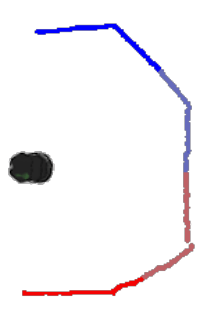
\includegraphics[width=0.2\textwidth]{slike/Fig04_06a.png}}
    \hfill
    \subfloat[Experimental results\label{fig:UshapeRes}]{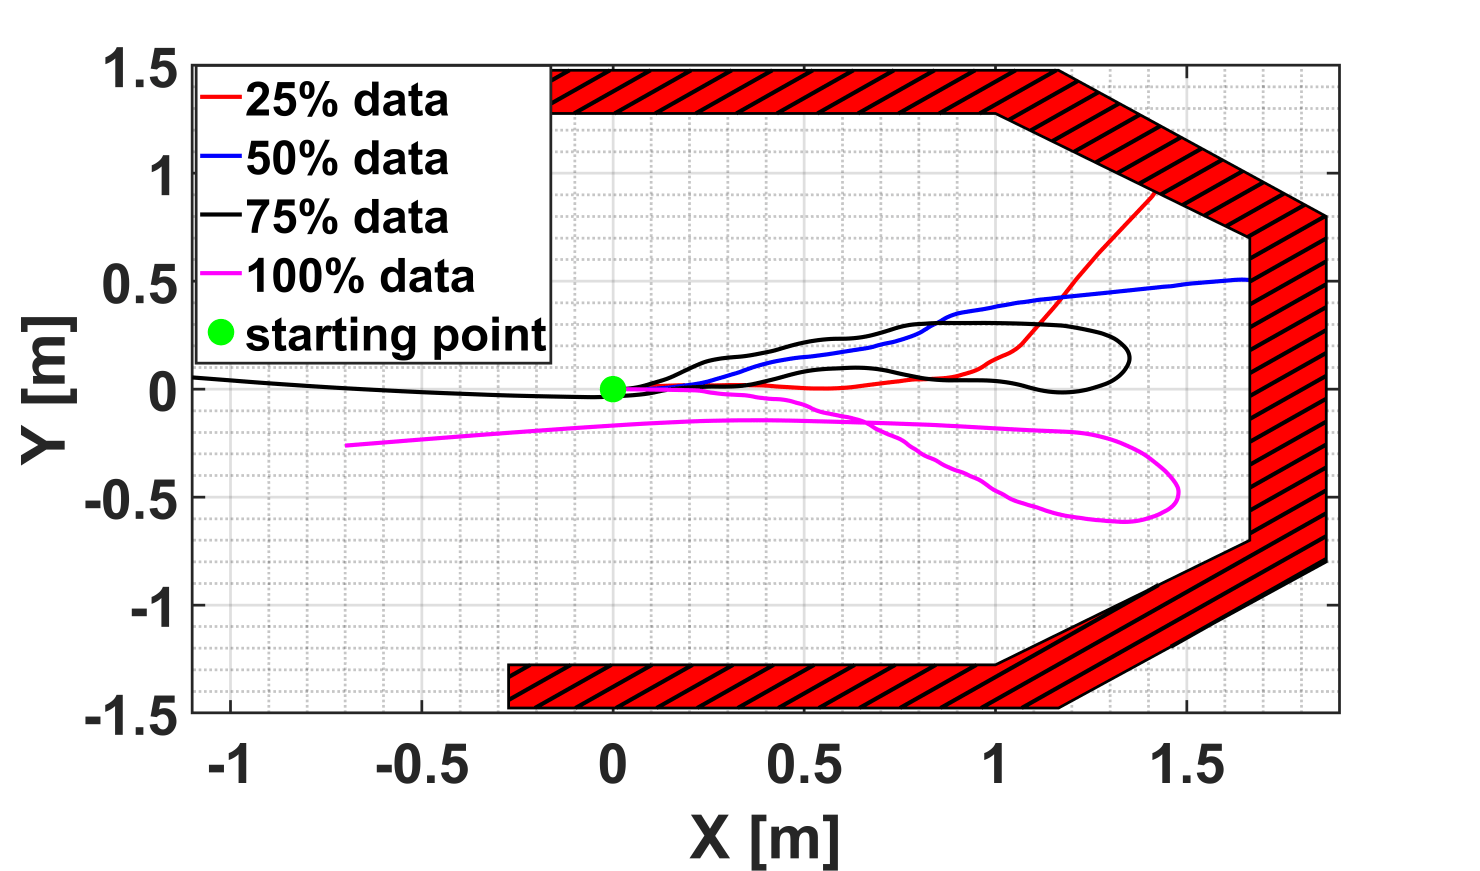
\includegraphics[width=0.66\textwidth]{slike/Fig04_06b.png}}
    \caption{Performance of the obstacle avoidance in the presence of a U-shaped obstacle}
    \label{fig:Fig09}
\end{figure}

It should be noted that for this scenario, the robot crashed at least once for all cases (with 25 \% data 3 out of 5 times, with 50 \% data 3 out of 5 times, and with 75 \% data 1 out of 5 times). The exception was for the case where the whole dataset was used. In contrast, any reduction in training data resulted in reduced reliability (especially in 25 \% and 50 \% test cases).

These results led to the conclusion that the amount of collected crash data is just right, but perhaps even more crash data could prove beneficial for the reliable performance of obstacle avoidance in such challenging situations. It should also be noted that convex dead-ends pose a particular problem to the proposed obstacle avoidance approach. However, the approach is not intended to be used all by itself. Instead, it should be used in conjunction with navigation to the given goal, shown later on.

\subsubsection{The narrow corridor course}

This experiment consisted of 20 test cases (5 repetitions for each of 4 neural network setups, as in the U-shape obstacle course), in all of which the robot did not pass the corridor as was intended (\cref{fig:Fig10}), signalling that there is still room for improvement. However, two interesting observations were made during the experiments. 

First, in 25 \% and 50 \% cases, the robot performed a U-turn and thus did not crash with the obstacle. However, this behaviour was not the desired one, but strictly speaking, it did avoid obstacles, which is the method's goal. 

Finally, for the 100 \% case, the robot moved the fastest but crashed with the final obstacle in all 5 test cases. However, it was observed that in all such cases, a crash occurred because the obstacle was too close to the robot’s right-hand side (while the robot started moving left and forward), so when it started to turn right, it simply did not notice the obstacle due to LiDAR minimum range issues and the way we processed such data. Thus, it can be considered a drawback of the sensor rather than a method (which could be reduced or eliminated with additional sensors like ultrasound range finders).

\begin{figure}
    \centering
    \subfloat[Raw LiDAR scan]{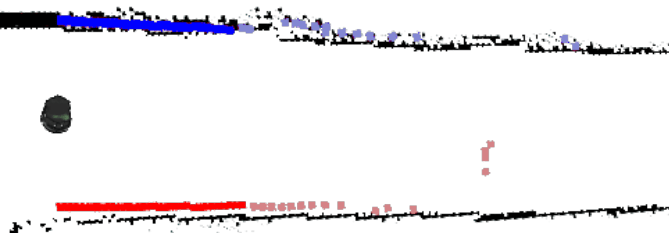
\includegraphics[height=0.2\textheight]{slike/Fig04_07a.png}}
    \vfill
    \subfloat[Results\label{fig:Fig10c}]{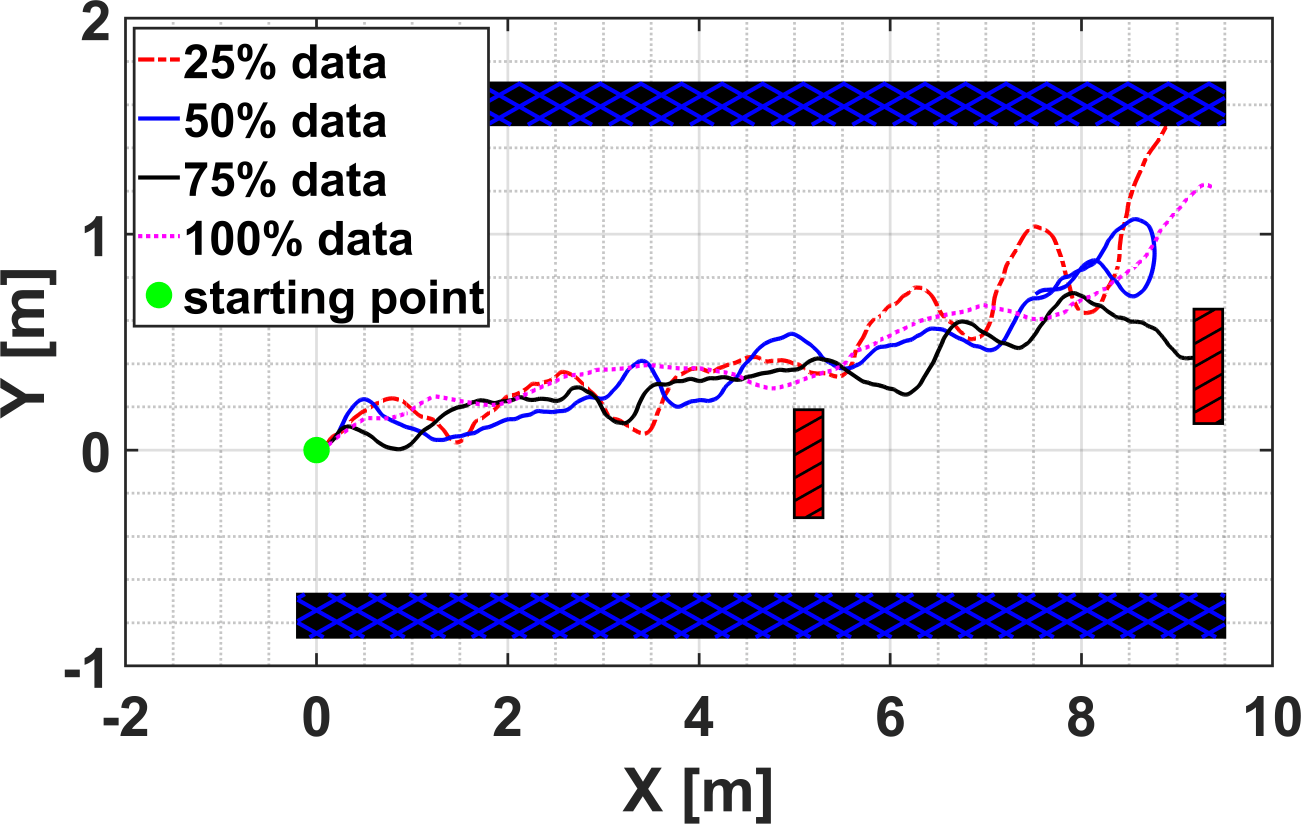
\includegraphics[width=0.75\textwidth]{slike/Fig04_07b.png}}
    \caption{Performance of the obstacle avoidance in a narrow corridor}
    \label{fig:Fig10}
\end{figure}

\subsubsection{Comparison with baseline}

This experiment was repeated three times for each algorithm (neural network-based obstacle avoidance and DWA), six times in total. The obtained trajectories are shown in Figure \ref{fig:Fig11}. However, only four of those are shown in the figure for clarity reasons. It should be noted that DWA always avoided the obstacle to the left, while the presented obstacle avoidance (in selected examples) chose the right side twice and the left side once (demonstrating the stochastic nature of the approach). The experiment demonstrated that the proposed approach could be integrated into navigation-based algorithms and perform well. In Figure \ref{fig:Fig11}, please note parts of the trajectories for neural network-based obstacle avoidance outlined with different colours, in which the neural network-based obstacle avoidance was in complete control of the robot (otherwise, the navigation part was in control or the control was shared).

\begin{figure}
    \centering
    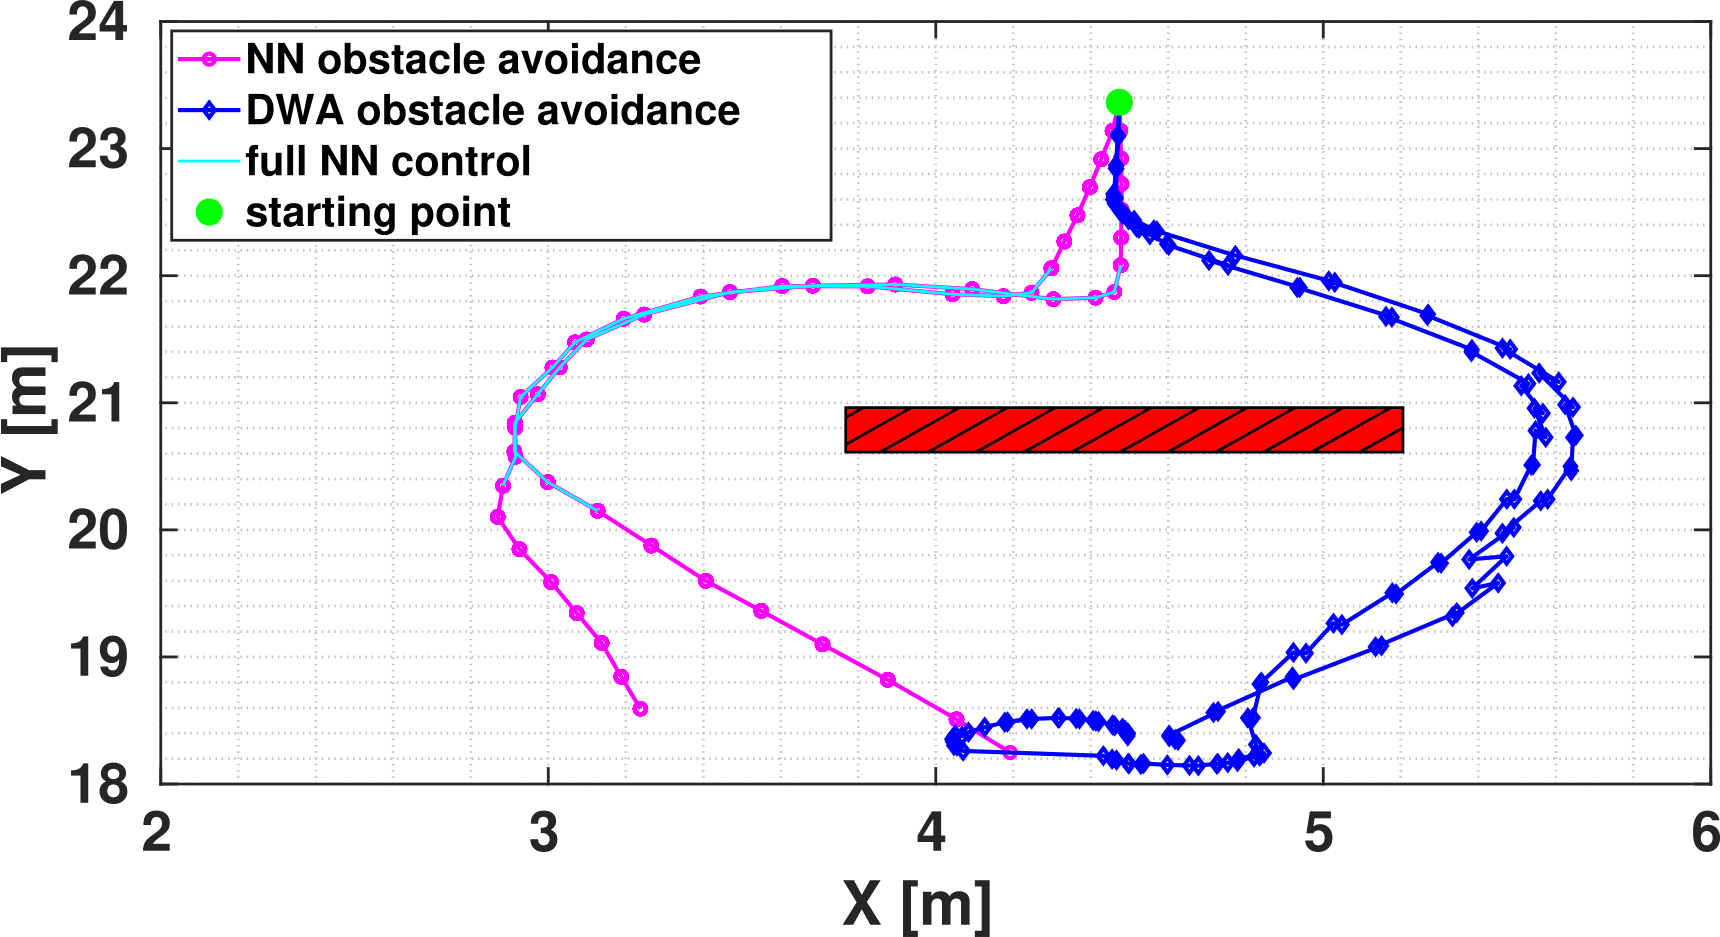
\includegraphics[width=0.75\textwidth]{slike/Fig04_08.png}
    \caption{Comparison of obstacle avoidance methods in a navigation task}
    \label{fig:Fig11}
\end{figure}

\subsubsection{Complex obstacle course}

In the complex, self-contained obstacle course (a snapshot of which is shown in \cref{fig:ObstacleCourseSnap}) that contained both static and moving obstacles, the obtained results were as follows: 8 collisions, 127 s ($\pm$ 102.88 s) for average time between collisions (and standard deviation), and 21.59 m ($\pm$ 17.49 m) for the average distance between collisions (and standard deviation). This performance is somewhat worse than simulation (in which there were no moving obstacles and had a smaller number of obstacles per meter squared - $0.194$ vs $0.223$), but still one that shows that the approach is valid and has potential for practical applications. Obtained results are also in line with results from \cite{Gandhi2017} for time and somewhat lower for distance. It should be kept in mind that our test scenario was cluttered with many obstacles, a case which would not be expected in everyday applications, and the one not used in \cite{Gandhi2017}. In standard office setup and uncluttered corridors, the neural network-based obstacle avoidance performance was improved. Also, out of 8 crashes, 4 of them were with moving obstacles (in cases when it was moving directly toward the robot with higher speed, again in line with results obtained from simulation with a single moving obstacle) and 1 with static obstacles with a very slim profile (less than five scan points needed for detection of obstacles in this approach, shown in \cref{fig:ObsCourseThin}). 

\begin{figure}
    \centering
    \subfloat[An overview of the course with moving obstacles]{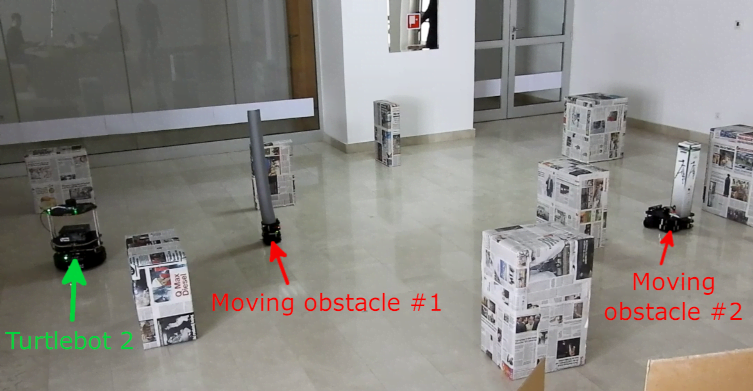
\includegraphics[width=0.75\textwidth]{slike/Fig04_09a.png}}
    \vfill
    \subfloat[A crash with an obstacle with a thin profile \label{fig:ObsCourseThin}]{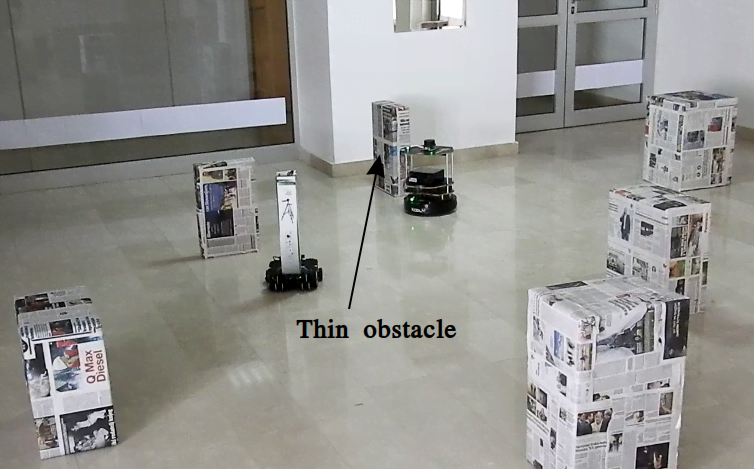
\includegraphics[width=0.495\textwidth]{slike/Fig04_09b.png}}
    \hfill
    \subfloat[A robot approaching the edge of the course]{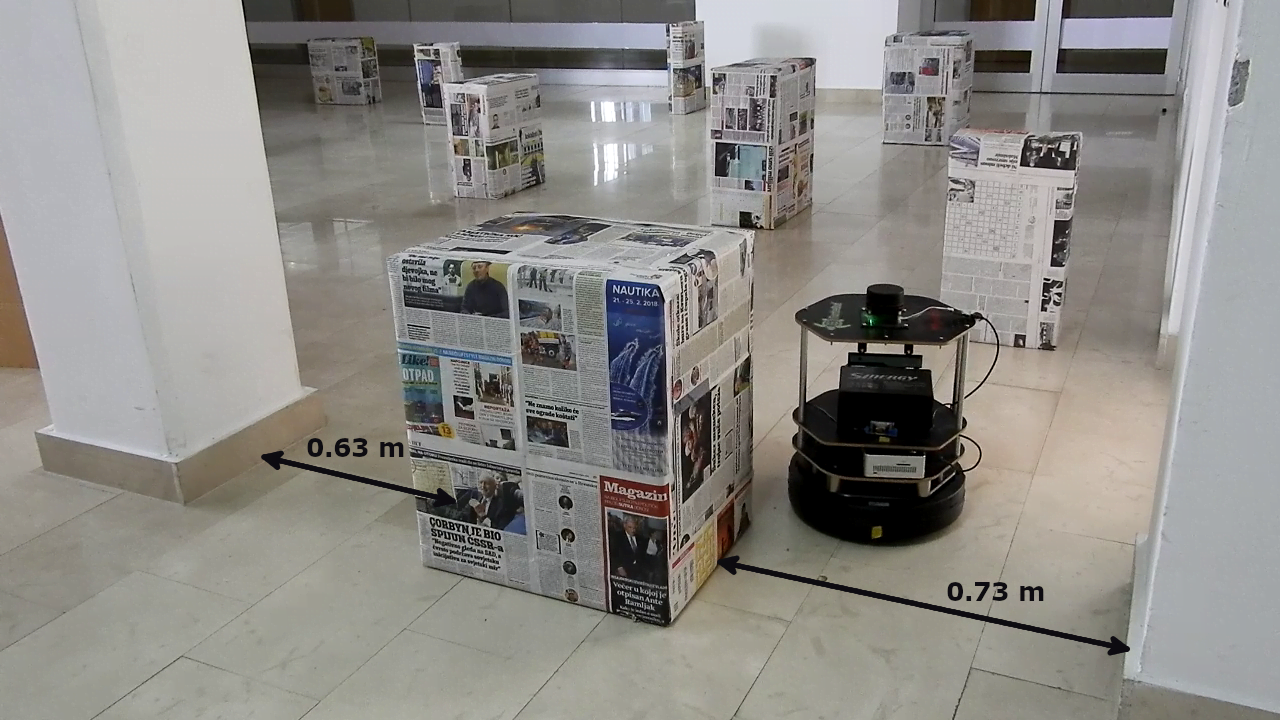
\includegraphics[width=0.495\textwidth]{slike/Fig04_09c.png}}
    \caption{Snapshots of real-world testing environment for obstacle avodaince in a complex obstacle course}
    \label{fig:ObstacleCourseSnap}
\end{figure}

Some of the crashes could have been avoided with a slightly different setup (e.g., lower number of scan points) and different and better trained neural networks (e.g., for going backwards or training on the more extensive and more diverse dataset). Another possible improvement is a unification of the three neural networks into a single neural network for possible smoother trajectories. 

When considering possible improvements of the proposed obstacle avoidance method, three additional possibilities were noted. First, since several crashes occurred with moving obstacles, adding moving obstacles into the simulation environment when generating data could benefit training. Secondly, the middle part of the obtained data discarded in training could be used as additional training examples for improved network performance. Finally, as in \cite{Zhu2017}, variations in shape and configuration of the training and test environments could potentially lead to improved performance.

\section{Mediated navigation in mobile robotics}
\label{sec:ResMediation}

The results reported throughout Section \ref{sec:ResMediation} are summarised in Table \ref{Tbl:ResultsSummary} for easier reading. They will be explained in more detail in the following subsections. Please note that only summary statistics regarding distance and time were reported in the table, and that raw results about specific experiment instances is provided at appropriate places in the following subsections. At the bottom of the table, there are two rows that summarise all the results in this section: one gives about total distances and timings in all experiments together and reports the total number of experimental trials, and the other states the percentage of total that is conducted using approaches proposed in this dissertation. These totals indicate the extent to which the proposed approach was tested. However, please keep in mind that all the testing was conducted indoors.

\subsection{Simulation} \label{sec:MediationSimResults}

Example trajectories (random $10$ out of $15$ for both test cases) obtained in the simulation are presented in Figure \ref{fig:SimulationTest}. Please note that goal points are marked with different symbols in each case.

It is worth noting that the mobile base never crashed for the neural network-based navigation controller, while for the P-type-based navigation controller, in four cases (26 \%) crash occurred. Due to the observed robot behaviour during the experiment, the conclusion was drawn that this was mainly due to the ``aggressive'' nature of the P-type controller (especially in rotation, when trying to reach the goal as directly as possible, ideally in a straight line), which tries to get to the goal point in a straight line. In contrast, neural network-based navigation tries to do the same but with a slightly arched trajectory, as can be seen in \cref{fig:SimulationTest}. Such behaviour makes it hard for neural network-based obstacle avoidance to recover (or even results in LiDAR failure due to an obstacle being too close). However, additional parameters, like goal points too close to the obstacles or in physically unreachable cases, might have, in some instances, contributed to the crash event. 

\begin{table}
\caption{Summary of all experimental results for the mediated navigation}
\label{Tbl:ResultsSummary}
\centering
\resizebox{\textwidth}{!}{%
\begin{tabular}{ccccccc}
\toprule
\textbf{Robot} & \textbf{Scenario} & \textbf{OA\tablefootnote{Obstacle avoidance controller used; NN--neural network, DWA--Default ROS obstacle avoidance controller}} & \textbf{Nav.\tablefootnote{Navigation controller used; NN--neural network, P--P-type controller, ROS--Default ROS navigation controller (Dijkstra), LF--Line following (Waypoint navigation)}} & \textbf{ADT}\tablefootnote{Average distance travelled} $\pm$STD [m] & \textbf{ATT}\tablefootnote{Average time taken} $\pm$STD [s] & \textbf{Trials} \\
\midrule
\multirow{2}{*}{\makecell{Turtlebot 2 \\ \emph{simulation}}} & \multirow{2}{*}{obstacle course} & NN & NN & 13.08$\pm$4.3 & 68.8$\pm$18.87 & \multirow{2}{*}{15 each} \\
 &  & NN & P & 7.44$\pm$3.32 & 38.4$\pm$16.15 &  \\ \midrule
\multirow{9}{*}{\makecell{Turtlebot 2 \\ \emph{real-world}}} & \multirow{3}{*}{Z-shape obstacle} & NN & NN & 8.75$\pm$1.89 & 43.76$\pm$1.94  & \multirow{3}{*}{5 each} \\ 
 &  & NN & P & 8.20$\pm$0.17 & 46.32$\pm$1.62 &  \\
 &  & DWA & ROS & 9.80$\pm$2.77 & 37.91$\pm$8.18 &  \\ \cmidrule{2-7}
 & \multirow{3}{*}{U-shape obstacle} & NN & NN & 12.25$\pm$0.69 & 69.15$\pm$3.75 & \multirow{3}{*}{5 each} \\
 &  & NN & P & 12.66$\pm$1.12 & 73.06$\pm$6.57 &  \\
 &  & DWA & ROS & 7.64$\pm$1.80 & 39.61$\pm$30.73 &  \\ \cmidrule{2-7} 
 & \multirow{3}{*}{navigation} & NN & NN & 51.11$\pm$14.55 & 316.78$\pm$29.32 & \multirow{3}{*}{2 each} \\
 &  & NN & P & 75.76$\pm$10.92 & 466.55$\pm$18.68 &  \\
 &  & DWA & ROS & 47.41$\pm$12.78 & 245.50$\pm$70.80 &  \\ \midrule
 \multirow{8}{*}{\makecell{custom built \\ \emph{real-world}}} & \multirow{3}{*}{obstacle course} & NN & NN & 13.37$\pm$2.89 & 73$\pm$13.11 & \multirow{3}{*}{3 each} \\
 &  & NN & P & 12.39$\pm$3.10 & 68.33$\pm$17.21 & \\
 &  & DWA & ROS & 13.93$\pm$1.79 & 110.33$\pm$11.50 & \\ \cmidrule{2-7} 
 & \multirow{4}{*}{navigation} & NN & NN & 47.55$\pm$15.95 & 301.5$\pm$112.43 & \multirow{4}{*}{2 each} \\
 &  & NN & P & 53.11$\pm$14.98 & 403.60$\pm$60.81 &  \\
 &  & DWA & ROS & 47.51$\pm$7.82 & 223.5$\pm$19.09 &  \\
 &  & NN & LF & 49.31$\pm$20.41 & 288$\pm$93.34 &  \\
 \midrule
 \multicolumn{4}{r}{\textbf{TOTAL}} &  1,466.78 & 8,401.29 & 83 \\
 \multicolumn{4}{r}{\textbf{USING THE PROPOSED APPROACHES (\%)}} &  78.27\% & 80.28\% & 79.52\% \\ 
 \bottomrule
\end{tabular}%
}
\end{table}



\begin{figure}
    \centering
    \subfloat[P-type navigation controller.\label{Fig:Gazebo_P}]{
        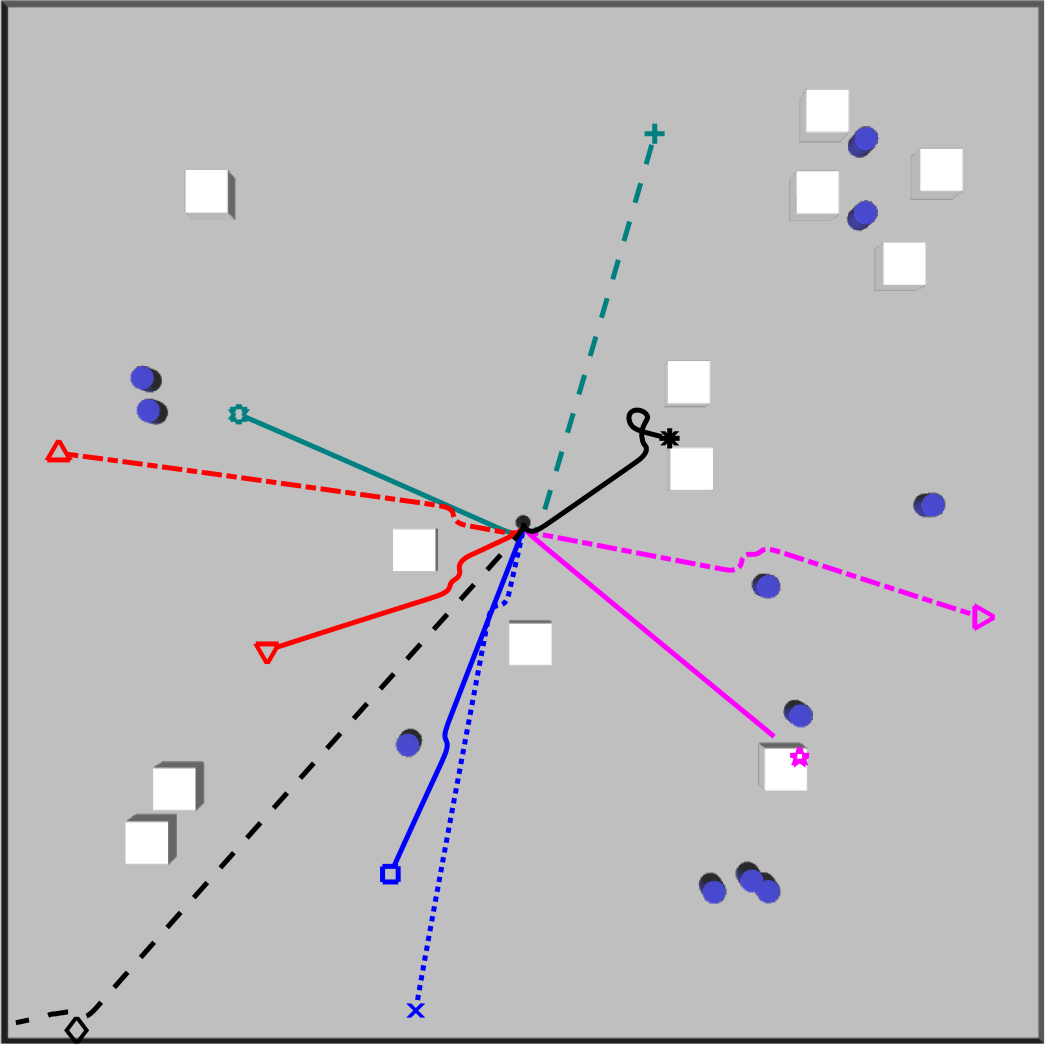
\includegraphics[width=0.475\textwidth]{slike/Fig04_10a.png}
    }
    \hfill
    \subfloat[Neural network-based navigation controller.\label{Fig:Gazebo_NN}]{
        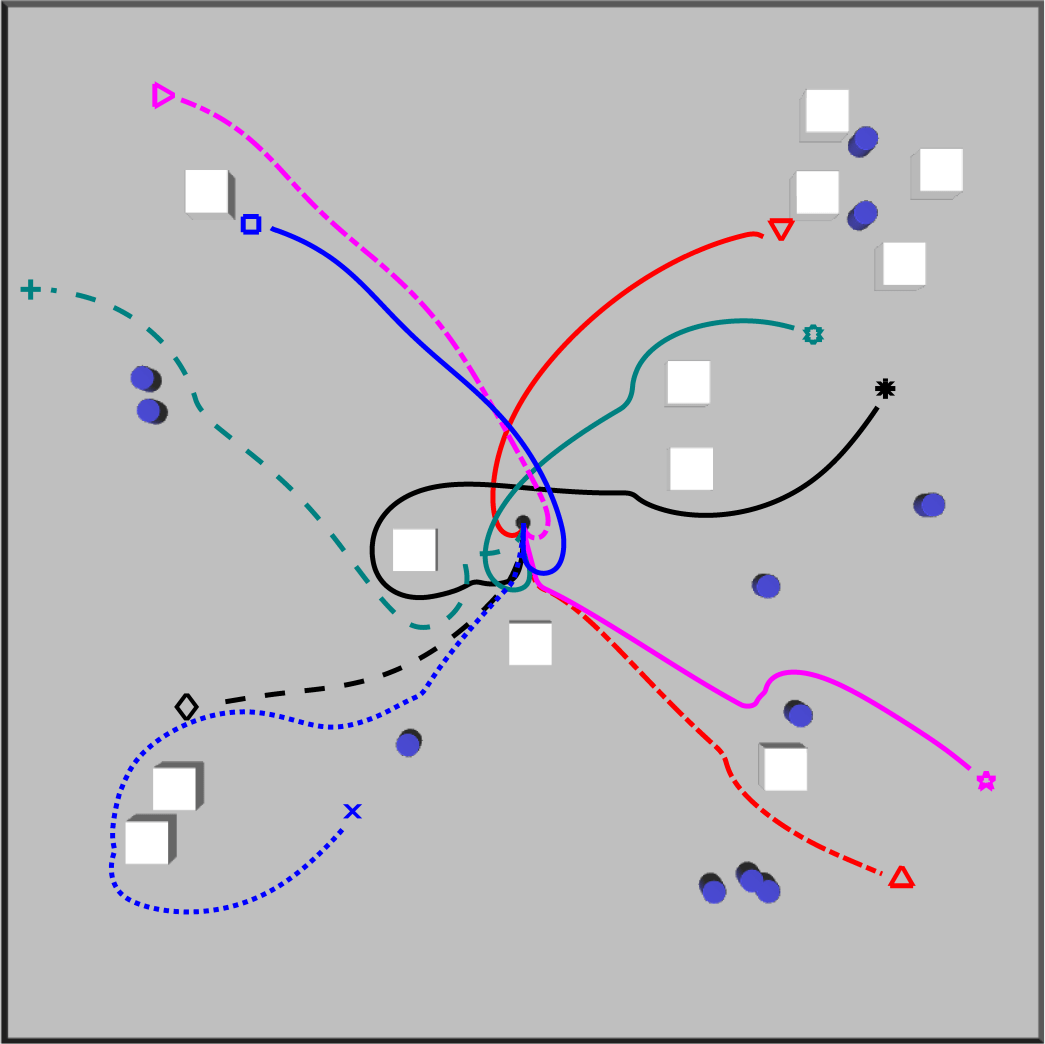
\includegraphics[width=0.475\textwidth]{slike/Fig04_10b.png}
    }
    \caption{Trajectories acquired during testing mediation in a simulation environment}
    \label{fig:SimulationTest}
\end{figure}

It is worth noting that the mobile base never crashed for the neural network-based navigation controller, while for the P-type-based navigation controller, in four cases (26 \%) crash occurred. Due to the observed robot behaviour during the experiment, the conclusion was drawn that this was mainly due to the ``aggressive'' nature of the P-type controller (especially in rotation, when trying to reach the goal as directly as possible, ideally in a straight line), which tries to get to the goal point in a straight line. In contrast, neural network-based navigation tries to do the same but with a slightly arched trajectory, as can be seen in \cref{fig:SimulationTest}. Such behaviour makes it hard for neural network-based obstacle avoidance to recover (or even results in LiDAR failure due to an obstacle being too close). However, additional parameters, like goal points too close to the obstacles or in physically unreachable cases, might have, in some instances, contribu6ted to the crash event. 

Looking at the presented trajectories in Figure \ref{fig:SimulationTest} several interesting observations can be made. First, the P-type controller results in a more direct approach to the goal (i.e., the ``aggressive'' nature mentioned before), while the neural network-based navigation takes a more circular trajectory even when the goal is in the line of sight with no obstacles in-between. From Figure \ref{Fig:Gazebo_P} it can also be observed that when the goal is too close to the obstacle (trajectory with the black dashed line and diamond goal marker), the robot might not reach its intended goal (since the mediation algorithm switches it to obstacle avoidance). Some improvement might be possible here if an adaptive collision probability calculation is employed using the remaining distance to the goal and the adaptive robot velocity (but clearly, there is a limit to this approach). Next, when the goal is placed within the obstacle (especially if it is within a corner type environment - pink line trajectory with a pentagram goal marker), the crash is inevitable since the obstacle avoidance does not react appropriately, i.e. there is no stop-and-turn in-place mechanism. This behaviour, however, does not seem to be the failure of the proposed fuzzy mediation approach (since it worked as intended) but highlights shortcomings of the developed obstacle avoidance approach (and ways of improving it, e.g. in-place rotation). Finally, if the target is close to the obstacle, but still far enough so that obstacle avoidance is not activated (black line trajectory with asterisk goal marker), it might take a while for a robot to reach the goal (switching several times between navigation and obstacle avoidance controller - note the end part of the trajectory), but it will reach it. Looking more closely at the Figure \ref{Fig:Gazebo_NN}, it can be seen once more that the robot does not take the most direct route and that obstacles sometimes interfere with the navigation (i.e. trigger the obstacle avoidance) as depicted by the black full line trajectory with asterisk goal marker and blue dotted trajectory with \emph{x} goal marker. This behaviour extends the distance travelled, but the robot ultimately reaches its goal, even when the goal point is close to the obstacle (trajectories with a red line with triangle end marker and a blue line with square end marker).

Despite several crashes, and based on the above discussion, it was concluded that the proposed fuzzy mediation algorithm is viable and performed as expected in the simulation. Thus, it was decided to deploy it in real-world scenarios and on real mobile robots.


\subsection{Simple real-world scenarios} \label{sec:MediationRWResults}

As was explained in Section \ref{sec:MediationReal} first real-world testing was carried out using a modified Turtlebot 2 mobile robot in case of Z- and U-shaped obstacles. Examples of the obtained trajectories for one random case per setup can be seen in Figure \ref{Fig:Trajektorije_prepreke} along with the associated collision probability and mediation coefficients. 

The figure shows that for all three setups, the robot reached the goal area (there was a small error in the end position when using the DWA obstacle avoidance controller, but this was contributed to AMCL and encoder related issues in the recorded data since the physical robot reached the target successfully). As expected, when using the DWA obstacle avoidance controller, the goal was reached in a more direct trajectory in both cases, while the proposed approach had a few direction changes due to the fusion of navigation and obstacle avoidance parts. Thus, again, a more ``aggressive'' nature of the P-type controller is seen: there are more direction changes in its trajectory than in the case of neural network-driven navigation, which is smoother. However, the proposed mediation algorithm performed as expected in all particular cases, enabling the robot to execute a simple navigation task. 

\begin{figure}
\centering
\subfloat[Trajectories (Z)\label{Fig:Trajektorije_preprekeA}]{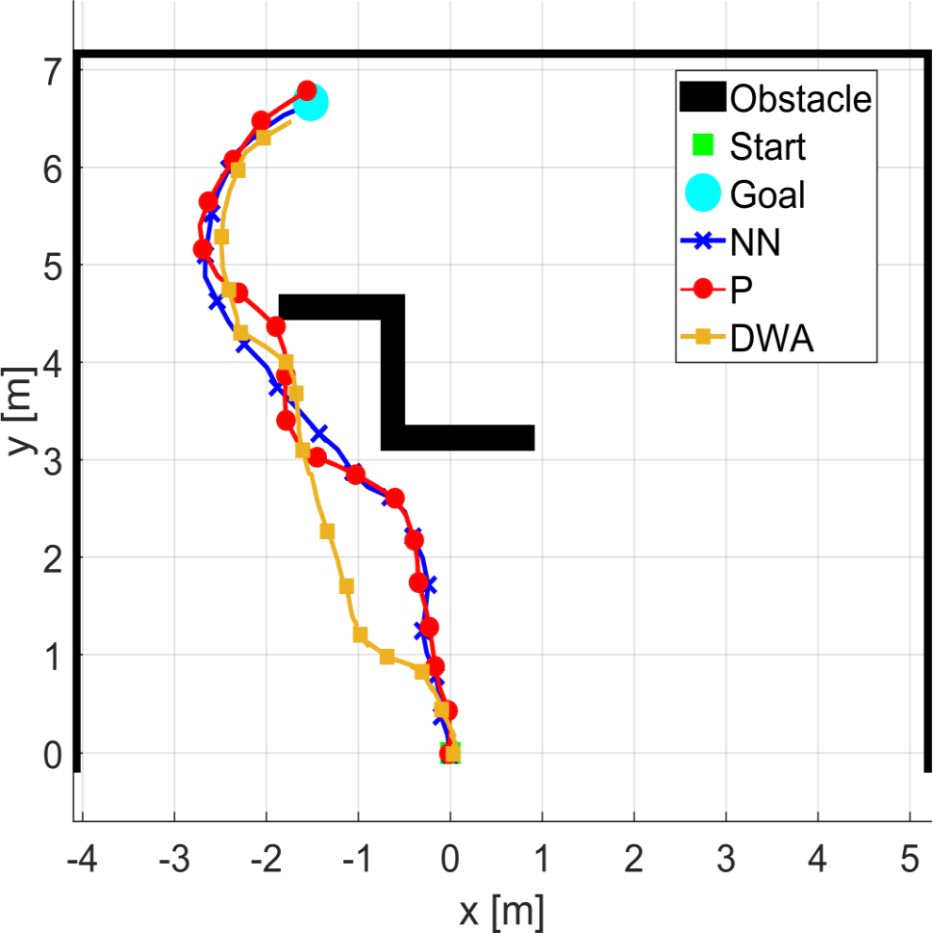
\includegraphics[width=0.45\textwidth]{slike/Fig04_11a.jpg}}
\hfill
\subfloat[$p_{col}$ and $\zeta$ values (Z)\label{Fig:Trajektorije_preprekeB}]{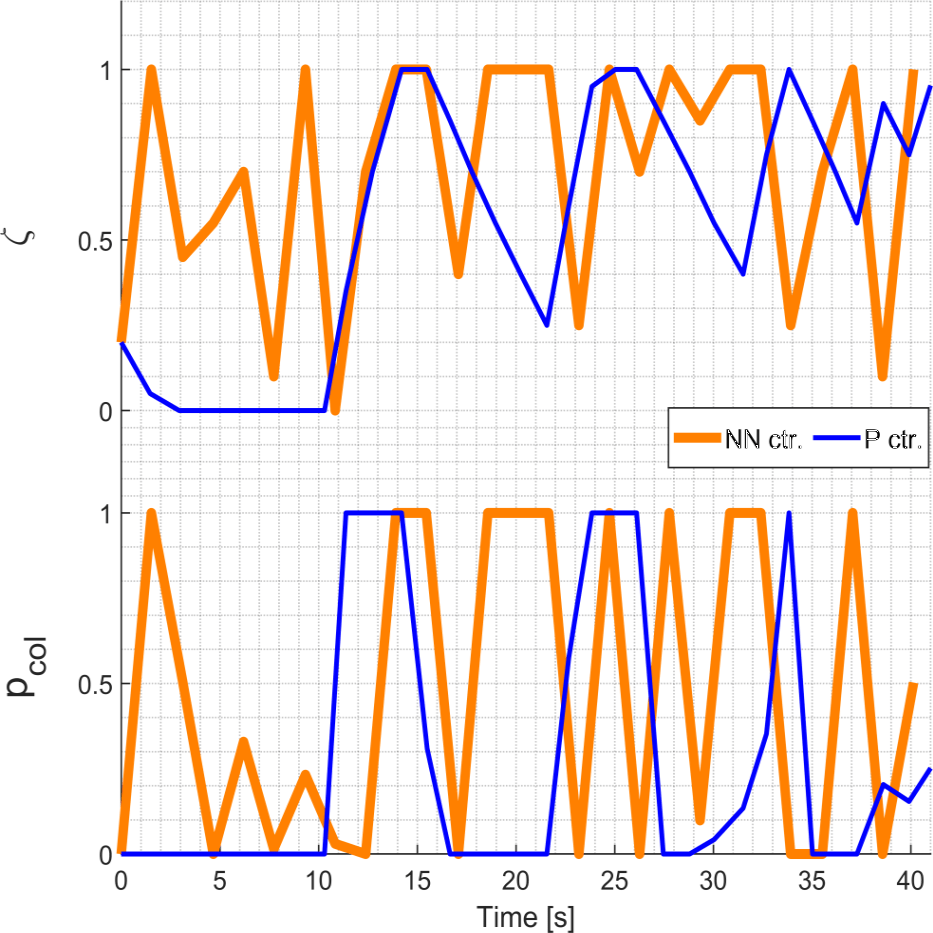
\includegraphics[width=0.45\textwidth]{slike/Fig04_11b.png}}
\vfill
\subfloat[Trajectories (U)\label{Fig:Trajektorije_preprekeC}]{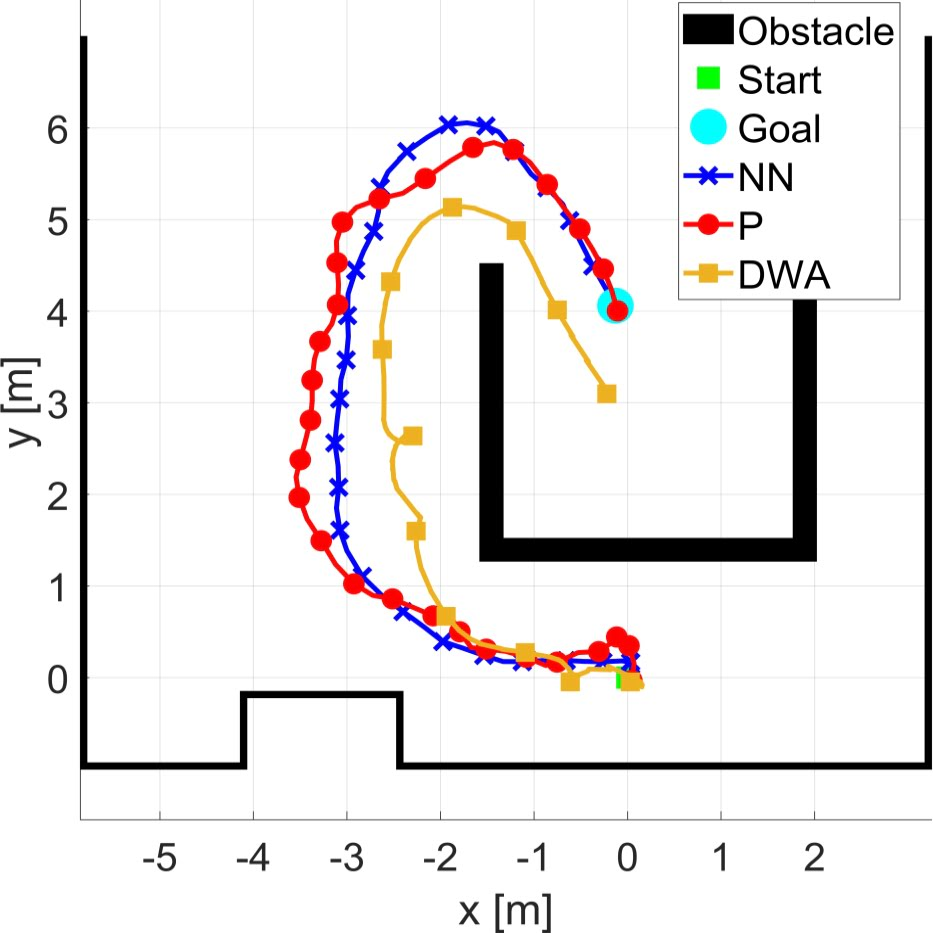
\includegraphics[width=0.45\textwidth]{slike/Fig04_11c.jpg}}
\hfill
\subfloat[$p_{col}$ and $\zeta$ values (U)\label{Fig:Trajektorije_preprekeD}]{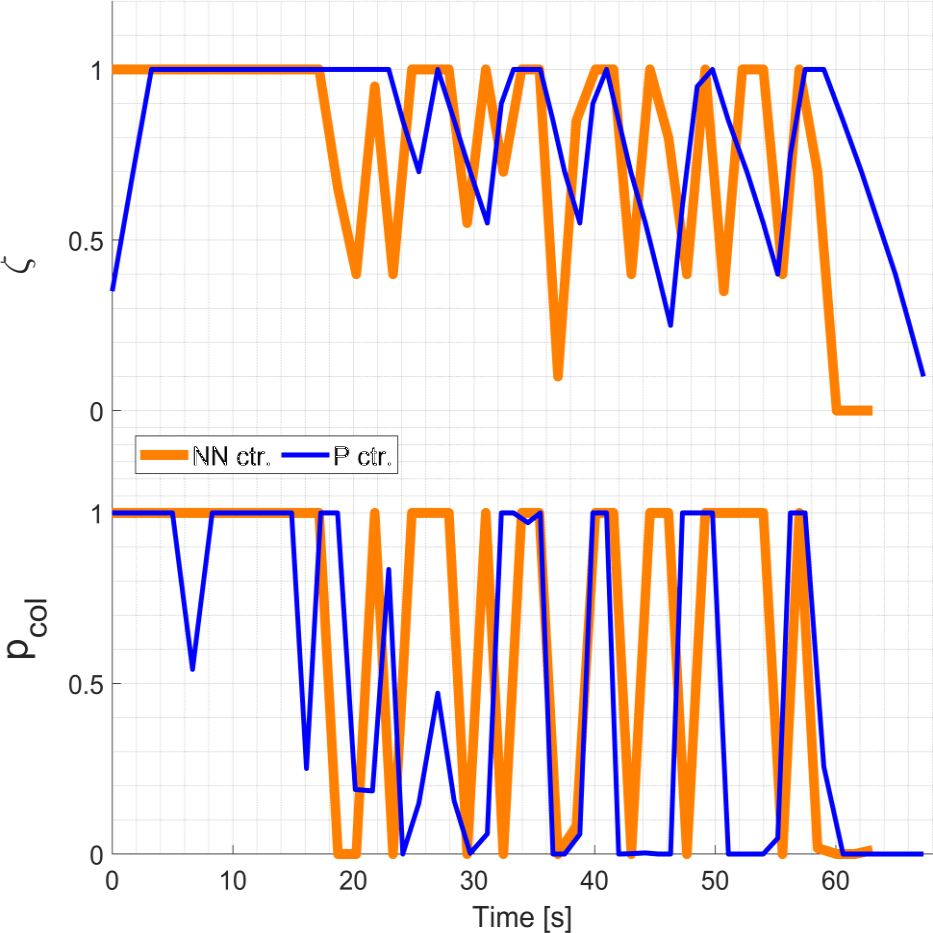
\includegraphics[width=0.45\textwidth]{slike/Fig04_11d.png}}
\caption{Examples of simple navigation task results with U- and Z-shaped obstacles.}
\label{Fig:Trajektorije_prepreke}
\end{figure}

It is interesting to note that DWA also had some issues with U-shaped obstacles. These issues resulted in longer navigation runs than both setups for the proposed approach (94.93 s vs 62.94 s vs 67.36 s for DWA, the neural network and P-controller setup, respectively). Completion times for the Z-shaped obstacle were similar for all three setups (DWA: 41.63 s, neural network: 39.06 s, and P-controller: 41.27 s, for this particular example). However, on average, ROS/DWA was the fastest method in all cases, but not always the one with the shortest distance travelled (please see \cref{Tbl:ResultsSummary}). In all experimental runs except one (for the U-shaped obstacle), the robot went left to avoid the obstacle and complete the course. In the mentioned single case, the robot went right to avoid the obstacle and into the narrow space (1.4 m) between the wall and the obstacle. Such decisions resulted in the longer run (102.32 s) with more direction changes because, during the entire run, the control was dominated by obstacle avoidance. These tests demonstrated that the proposed approach can be applied even in more demanding cases like the U-shape obstacle, but with certain limitations. Namely, the mediation approach lengthens the run due to the domination of the obstacle avoidance part. However, shortcoming could be avoided by using a more appropriate navigation controller with some waypoints on the way to the given goal, rather than just a goal point, as was the case in this experiment.

The change in the collision probability and $\zeta$ parameter values for both test cases (where the mediation was used) can be seen in Figures \ref{Fig:Trajektorije_preprekeB} and \ref{Fig:Trajektorije_preprekeD}. Please note that the value of $\zeta=1$ means that the obstacle avoidance controller is in complete control of the robot, and $\zeta=0$ is in pure navigation mode. All values in between mean that the mediation approach considers both the navigation and obstacle avoidance controller (in an appropriate proportion).

Next, a more demanding navigation task was used to test the proposed mediation approach in the larger environment and a realistic scenario. The experiment was conducted on the fourth floor at the University of Split, Faculty of Electrical Engineering, Mechanical Engineering and Naval Architecture, while Turtlebot 2 robot was used in the experiment. Examples of the obtained trajectories (for two different goal points) are depicted in Figure \ref{Fig:Trajektorije_hodnik}. Please note that although the obtained trajectories are plotted on the map, the robot itself did not have access to the map in the proposed approach (but does have it without obstacles for ROS/DWA case). In essence, robot path planning is a straight line, going from the start to the proposed approach's goal position. From the figure, it can be observed that the robot successfully reached the goals in all cases, with ROS/DWA again having a more direct route which is reflected in completion times in Table \ref{Tbl:ResultsSummary}. The main reason for this is that the upper corridor in which the robot had to enter was narrow (1.8 m) and resulted in the activation of the obstacle avoidance part, which turned the robot away from it if the approach angle was not appropriate. It is also evident that trajectories obtained using neural network-based navigation controller resulted (again) in smoother trajectories than those with P-type controller, which was a consequence of the ``aggressiveness'' of the P-type controller in trying to reach the goal. In terms of speed, i.e., completion time, the following results were obtained: 295.56 s and 195.44 s for DWA case, 337.51 s and 296.05 s for neural network case, and finally 479.76 s and 453.34 s for the P case. It should be noted that for specific start-goal point configurations, the robot got stuck at certain areas in space, constantly switching between obstacle avoidance and navigation. A similar effect was reported in \cite{Pfeiffer2017} and could potentially be reduced/eliminated by inserting several additional waypoints.

\begin{figure}
\centering
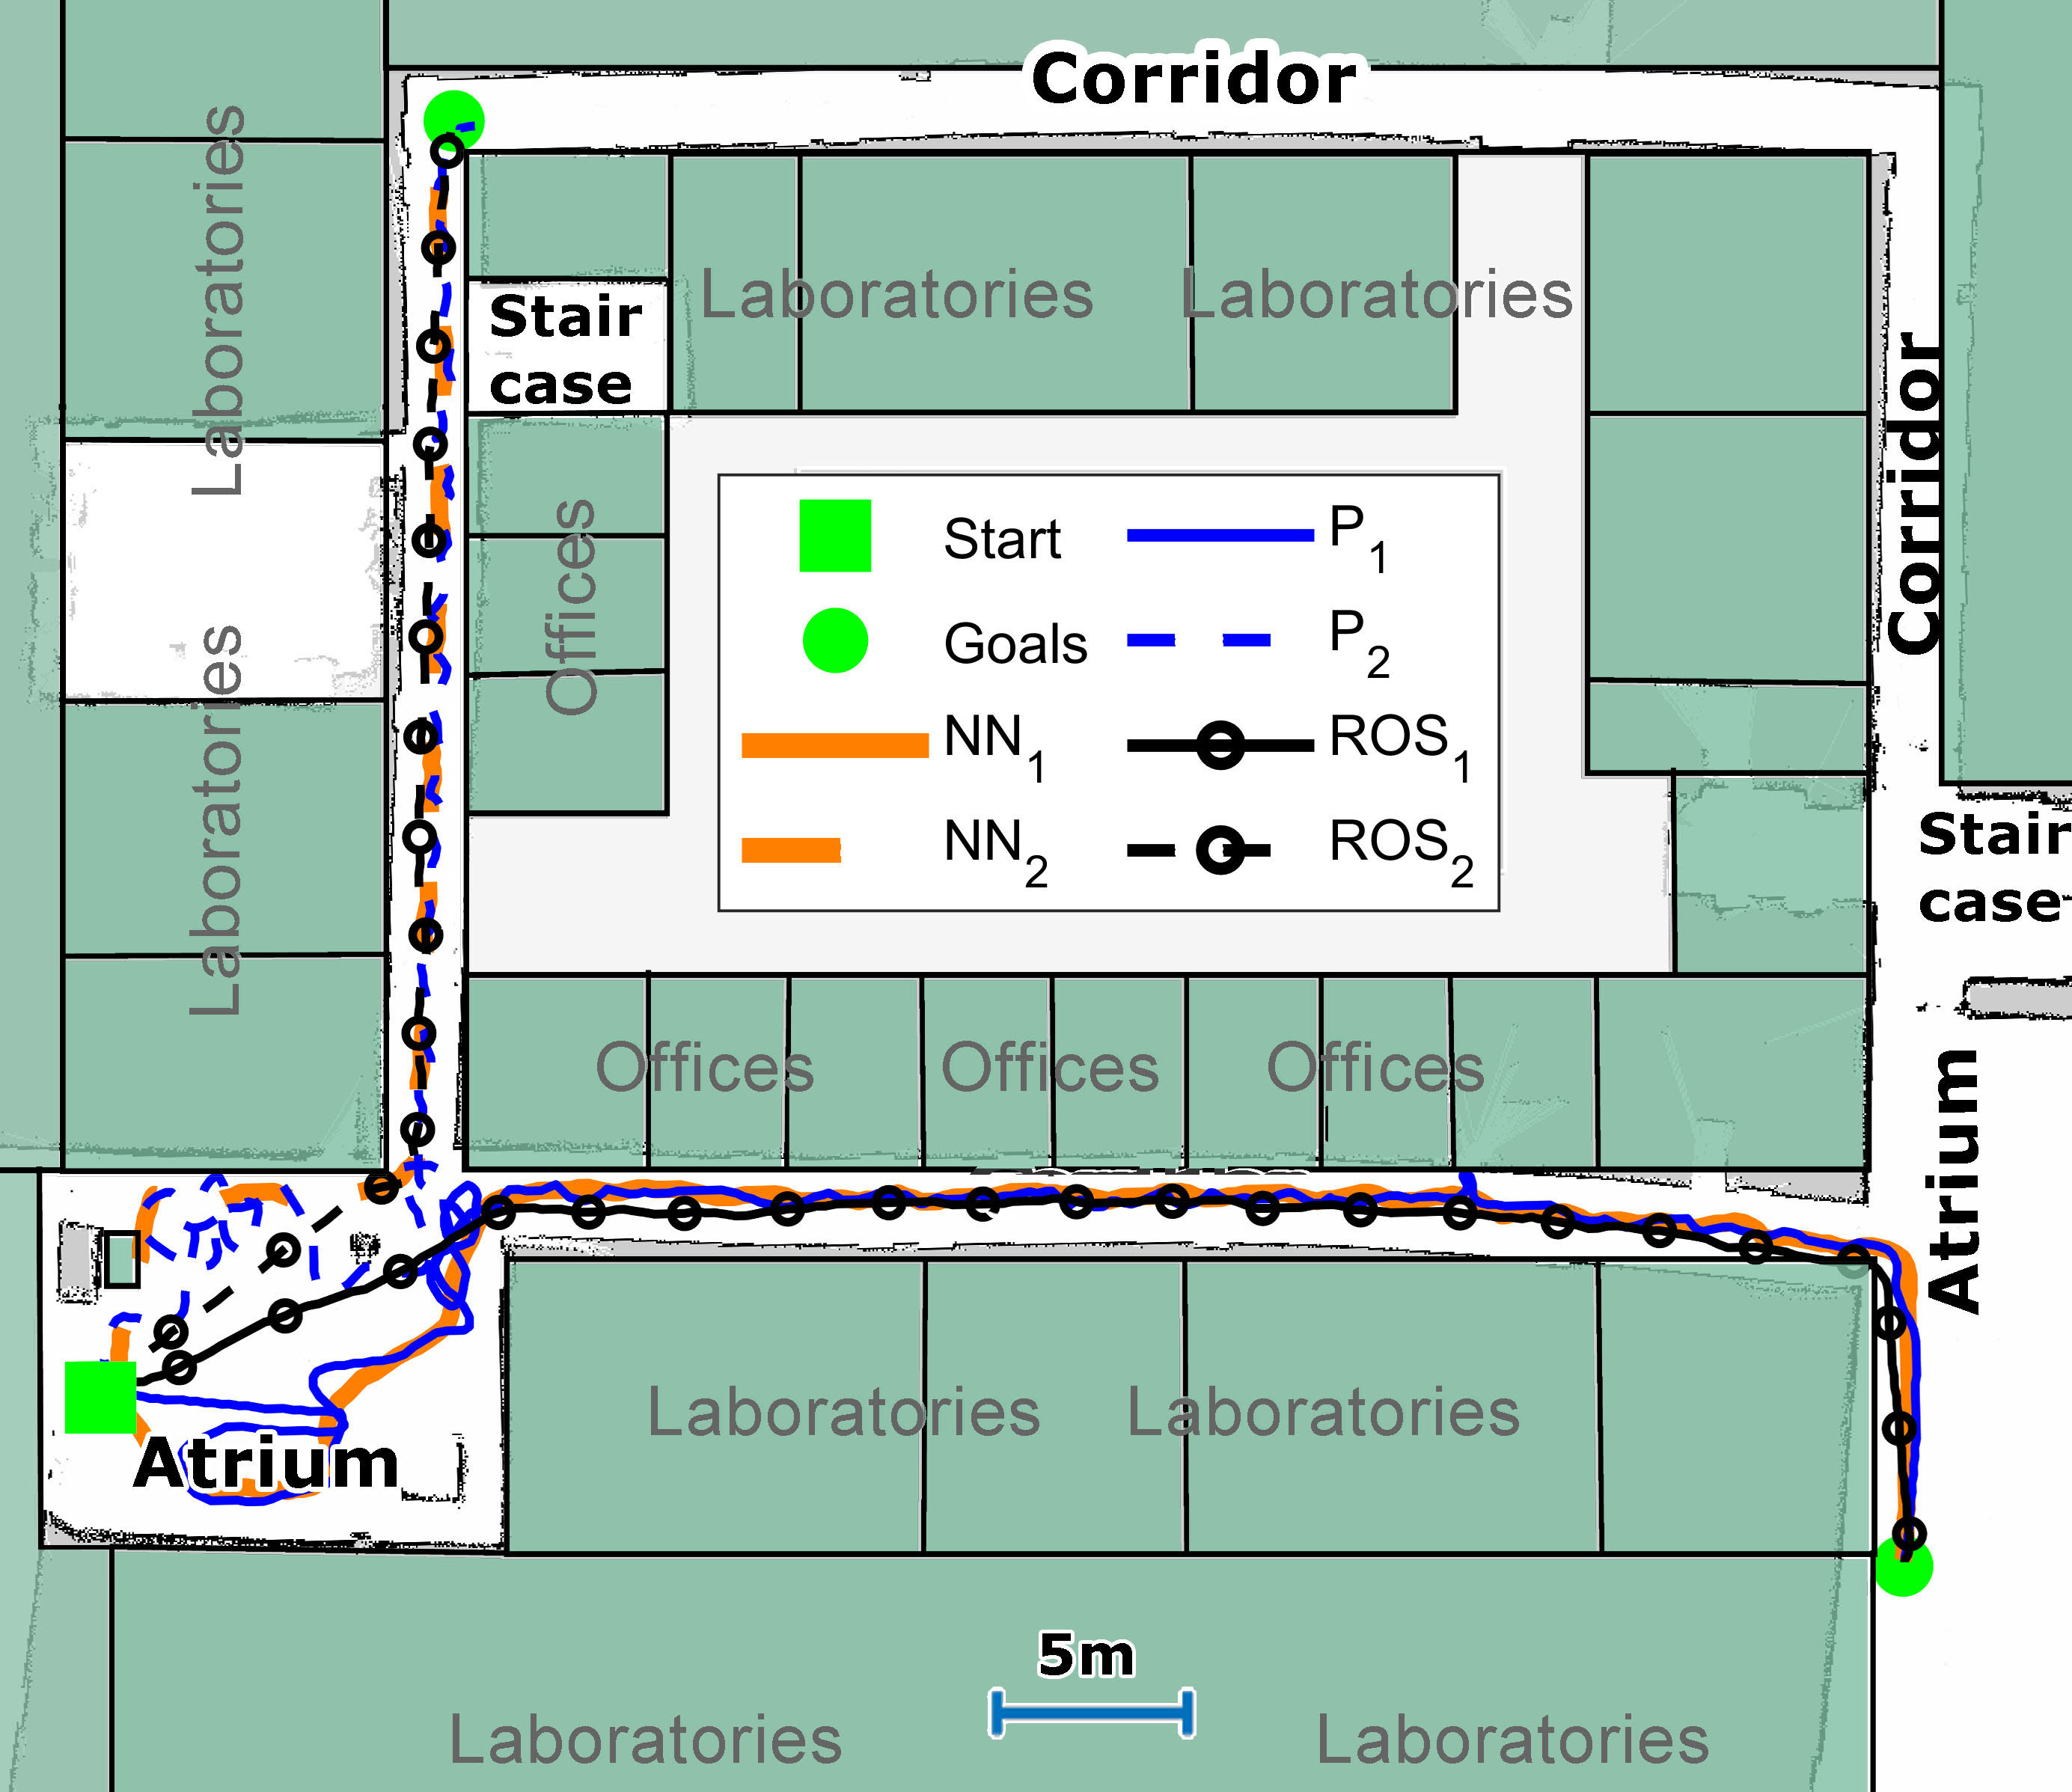
\includegraphics[width=0.85\columnwidth]{slike/Fig04_12.jpg}
\caption{Trajectories obtained in the demanding navigation task with Turtlebot 2 robot using different obstacle avoidance and navigation setups}
\label{Fig:Trajektorije_hodnik}
\end{figure}

In the next stage of testing, a custom-built robot with a different footprint was used. It was first tested on a more extensive obstacle course where it had to go from the start to a goal position. The experimental setup and the obtained trajectories are presented in Figure \ref{Fig:paletarTesting} and the obtained results are summarised in Table \ref{Tbl:ResultsSummary}.

\begin{figure}
\centering
\subfloat[Experimental setup \label{Fig:B401Mjerenje_NN}]{
   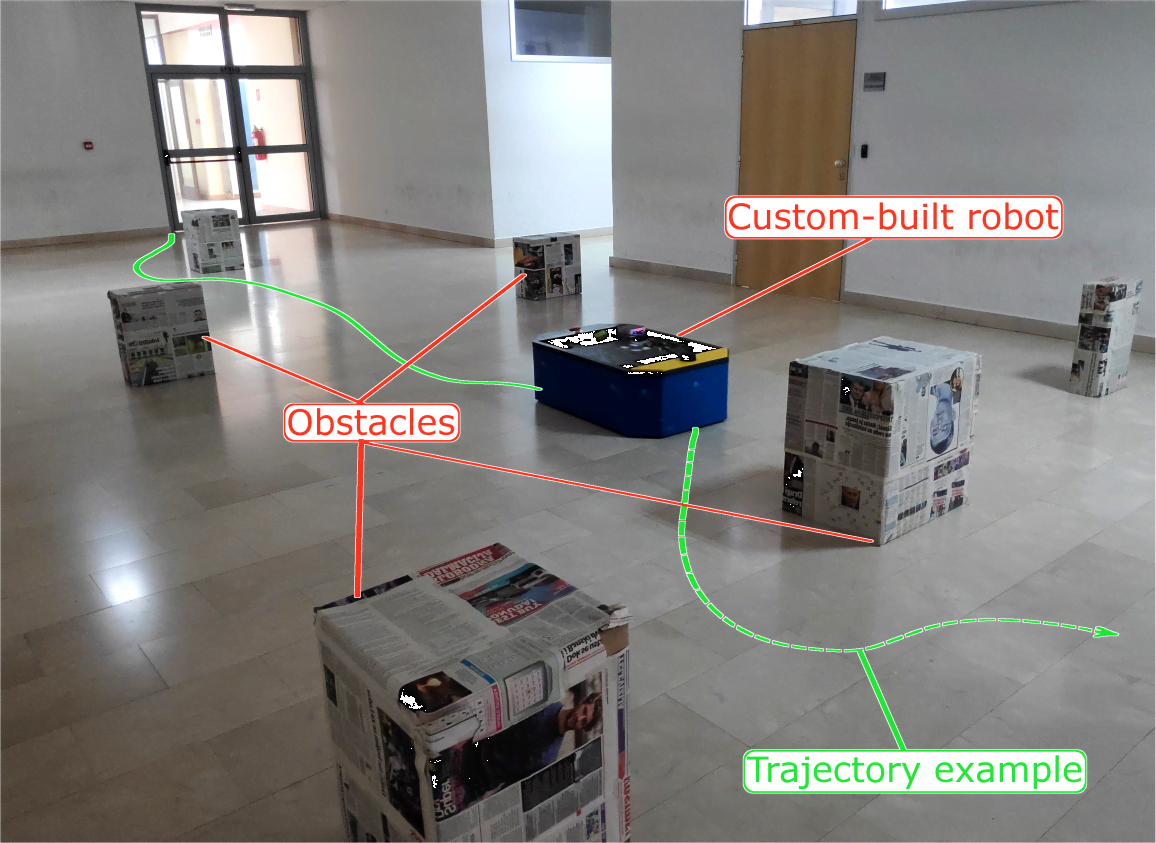
\includegraphics[width=0.8\textwidth]{slike/Fig04_13a.png}}
\hfill
\subfloat[Example trajectories with artificial obstacles marked as filled blocks (in scale)]{
   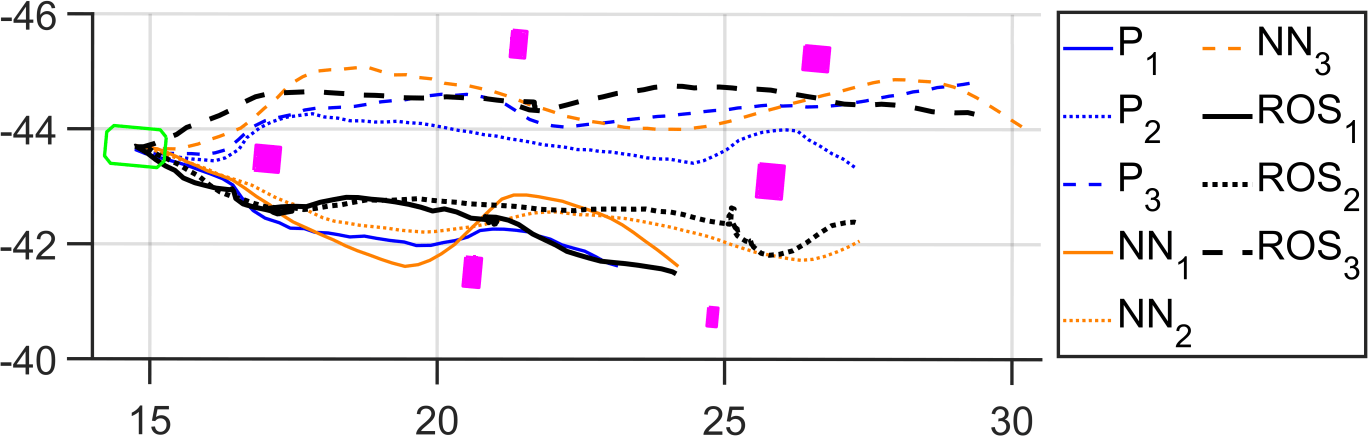
\includegraphics[width=0.98\textwidth]{slike/Fig04_13b.png}
   }
\caption{Experimental measurement with the custom-built robot on an obstacle course}
\label{Fig:paletarTesting}
\end{figure}

The results show that the robot successfully (i.e., without the crash) completed the task in all test cases. Please note again that the robot did not have access to the map in mediation test cases, while for ROS/DWA, it had but without obstacles. As in all cases before, the ROS/DWA seems to have a more direct trajectory. This more straight trajectory is, however, misleading since this approach had, in all cases, several in-place turns (which are not visible in the figure but are reflected in the time results in Table \ref{Tbl:ResultsSummary}) and even some backward driving (as seen in the figure in the case of bottom dotted black line trajectory). This observation is confirmed when completion times are examined (for goal points from top to bottom): the neural network-based navigation achieved times of 59 s, 75 s, and 85 s, the P-type navigation controller of 49 s, 74 s, and 82 s, while ROS navigation stack with DWA obstacle avoidance achieved 99 s, 122 s, and 110 s, respectively. Thus, it can be concluded, looking at the timings, that due to the more direct approach, the P-type controller achieved the fastest times and shorter distance travelled (Table \ref{Tbl:ResultsSummary}). Regardless of achieved times, the proposed fuzzy mediation algorithm performed as intended, mediating between two distinct robot behaviours. 

As the final test, a more complex navigation task with the custom-built robot was introduced. The experiment was conducted in the same environment as in the complex navigation task of the Turtlebot 2 robot. Obtained results are depicted in Figure \ref{Fig:Trajektorije_hodnik2}.

From the trajectories presented in the figure, it is clear that the robot completed the given task in all cases. However, how it was completed was slightly different, especially for the P-type navigation controller. To be more precise, the mobile robot, in that case, took numerous direction corrections (as can be seen best from the solid blue line trajectory) since it aggressively changed its direction, trying to reach the goal in a straight line. Thus, obstacle avoidance was engaged more often due to the robot's larger dimensions and the corridor width. However, this behaviour was not detected in neural network-based navigation, where the trajectory was smoother than using the P-type controller.

It should be noted that even the ROS navigation stack with DWA had several in-place rotations when coming into the narrow corridors. The following values are obtained if completion times are examined (to the first and the second goal point, respectively). The P-type controller finished the course in 446 s and 360 s, while the neural network-based navigation approach finished it in 381 s and 222 s.

On the other hand, the simple/custom line path planning and line following algorithm (with three waypoints going through the walls) finished the course in 354 s and 222 s, and ROS based navigation stack with DWA in 210 s and 237 s. Again, as before, it should be noted that better performance could be achieved by parameter optimisation of ROS/DWA method as well as our approach, but that was not the aim of the research. From the completion times for the P-type controller, the effects of numerous rotations and direction corrections are evident, having the slowest time in both cases (by a large margin). The remaining three approaches demonstrated comparable performance in the second goal point (right part of the figure), while the ROS/DWA-based approach was the fastest for the first goal point. Additionally, it was noted that adding waypoints, in general, decreased completion time and helped the proposed algorithm to deal with more complex situations (like convex dead-end obstacles). Regardless of these times, the performance demonstrated that the fuzzy mediation-based approach could produce good and reliable results even when a robot with a larger footprint is used in a realistic environment, especially with the addition of several waypoints.

Please note that improved/faster performance might be achieved if numerous ROS/DWA navigation stack parameters are better tuned: four DWA parameters had to be tuned during the experiments to get the algorithm to work correctly with the custom-built robot. On the other hand, for the mediation approach, the only parameters that were changed (alongside the adjusted footprint) compared to the Turtlebot 2 case were just the initial dimensions of uncertainty ellipses, as they needed to be increased due to the larger dimensions of the robot.

\begin{figure}
    \centering
    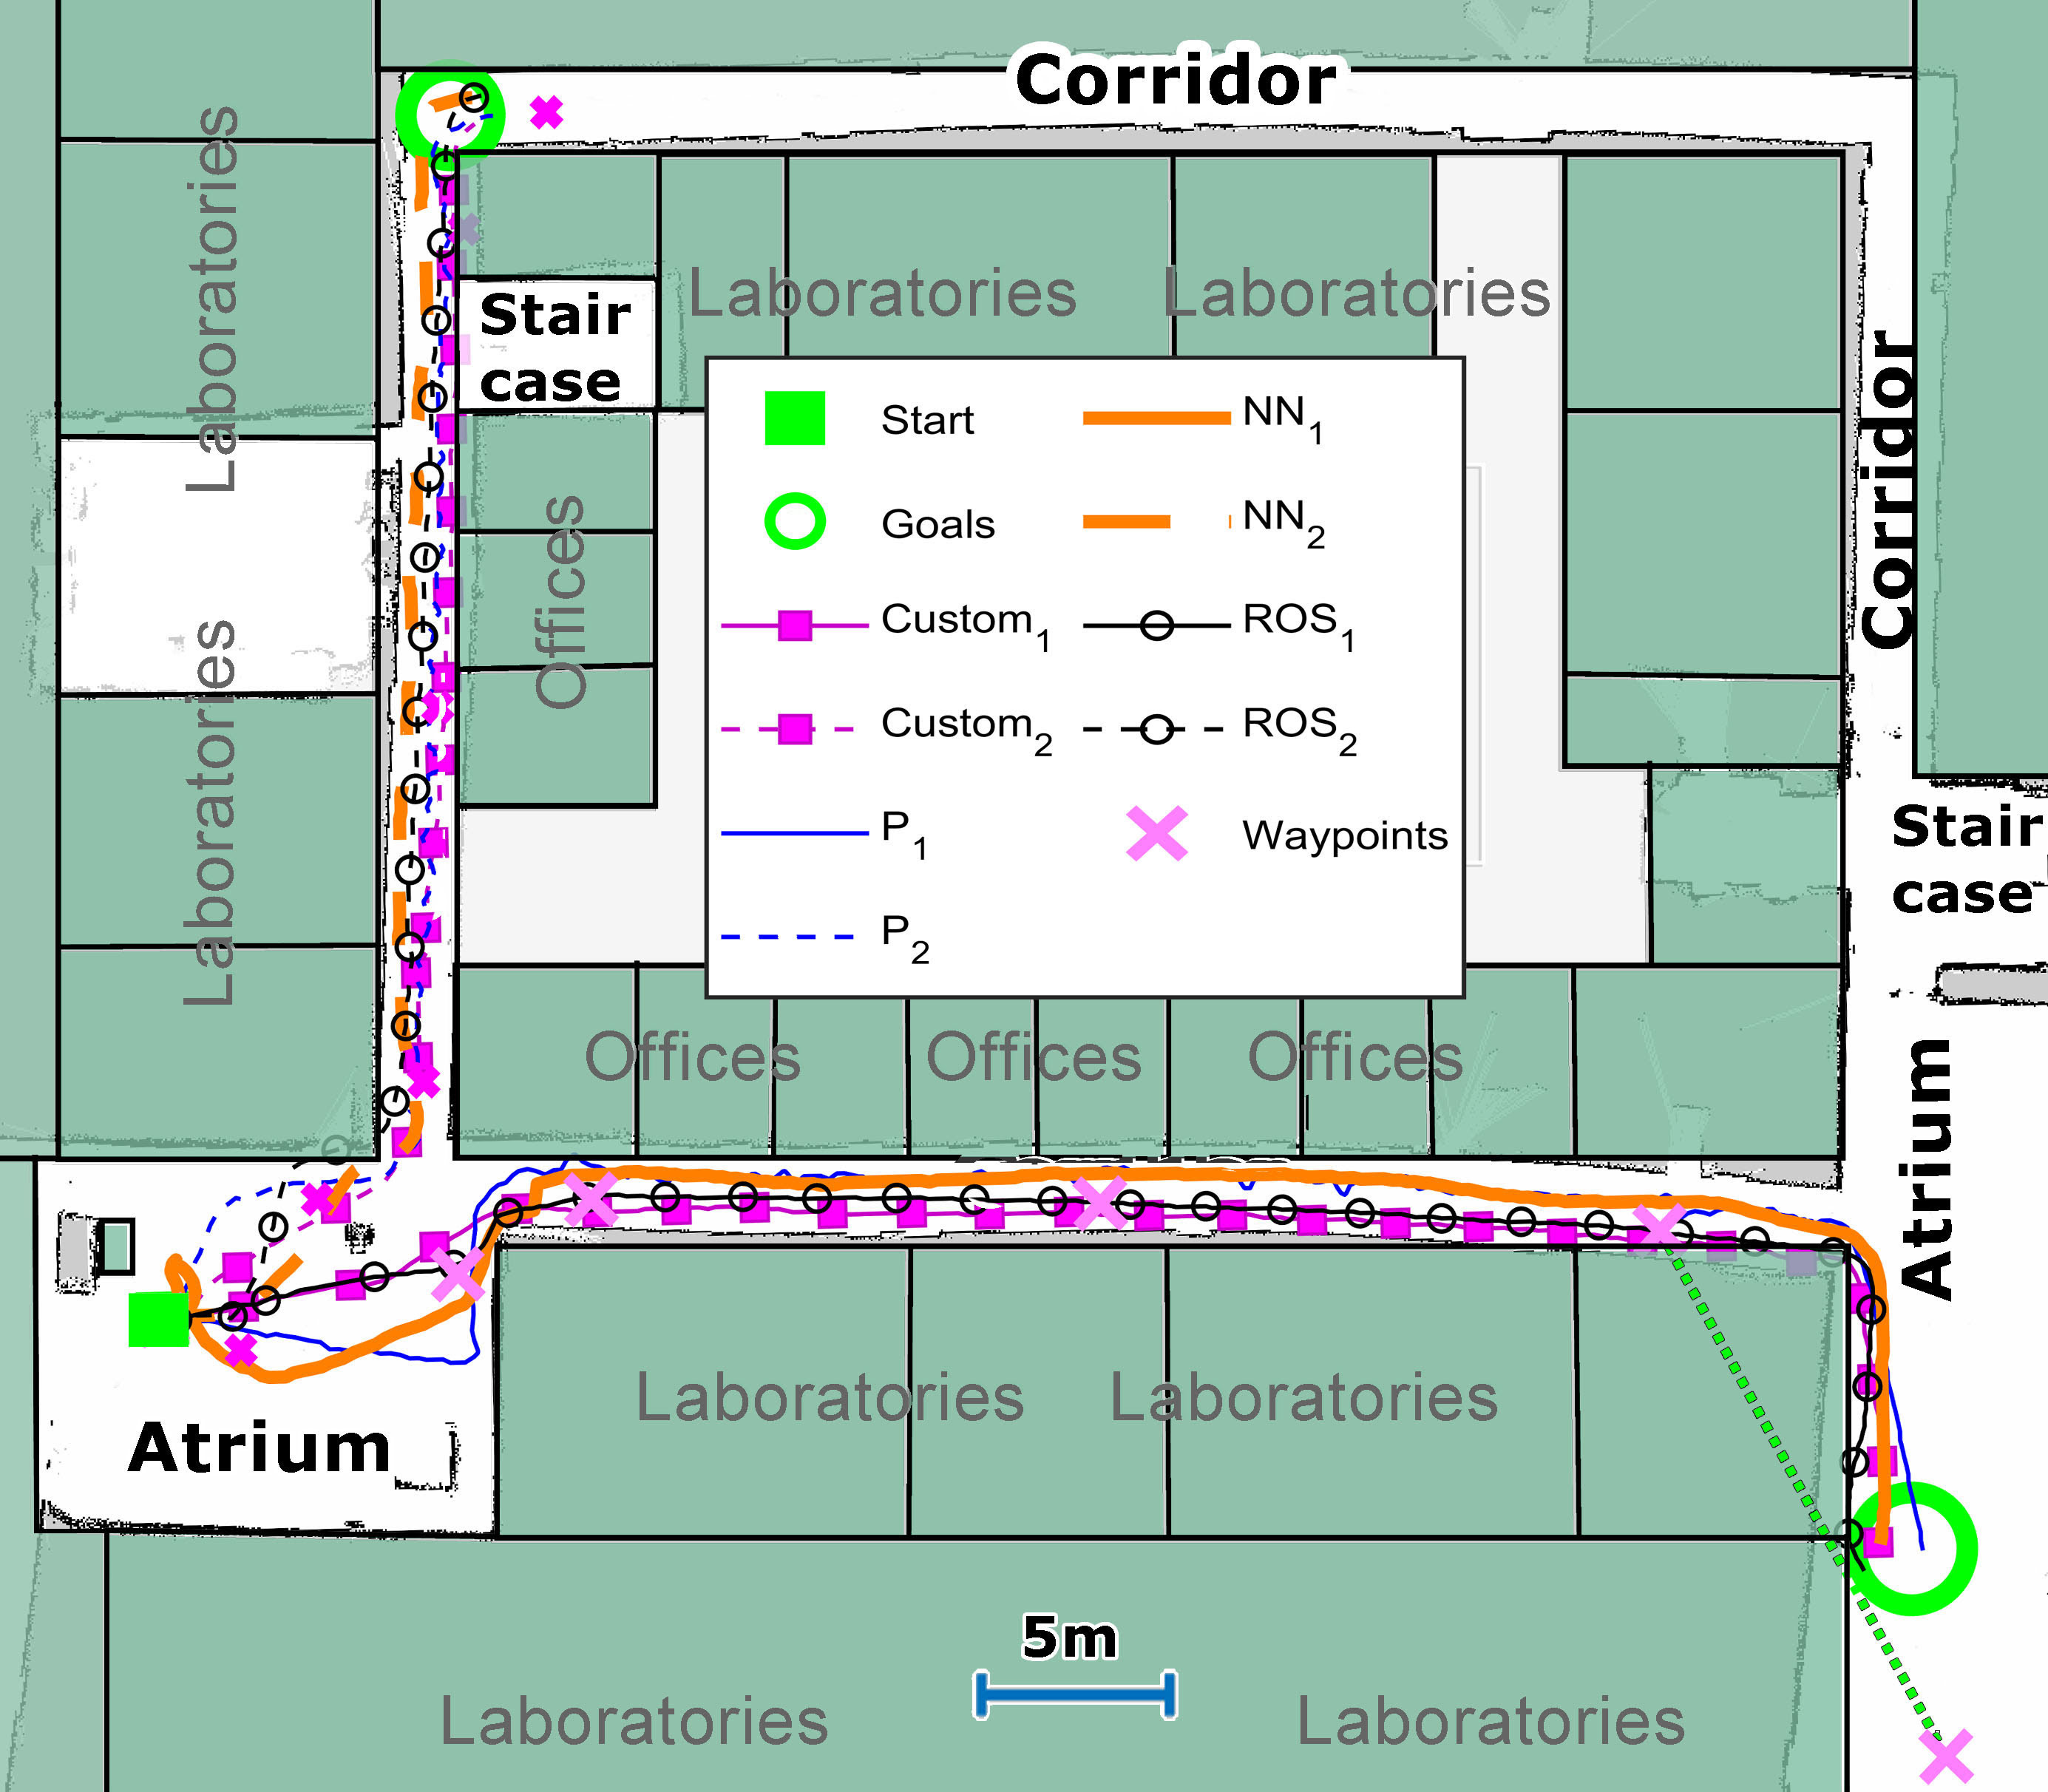
\includegraphics[width=0.85\columnwidth]{slike/Fig04_14.jpg}
    \caption{Trajectories obtained in the demanding navigation task with custom-built robot using different obstacle avoidance and navigation setups}
    \label{Fig:Trajektorije_hodnik2}
\end{figure}

\subsection{Teleoperation scenario} \label{sec:MediationTeleopResults}

During the application-based testing, subjects (students and faculty in author's institution) in all test cases completed the given task. However, in 100 \% of cases with \emph{surprise obstacles} case, the mediation algorithm activated the neural network-based obstacle avoidance, while in 47 \% of cases with \emph{no surprise obstacles} instances, the fuzzy mediation activated obstacle avoidance. This behaviour highlights the need for inclusion of such a safety mechanism (possibly fine-tuned by an operator) in teleoperation, since, with even one visible large obstacle (as was the case here), operators did not manage to complete the task without the danger of damaging either the robot or the obstacle. It should, however, be noted that in 23 \% of all cases, when the mediator transferred the control to obstacle avoidance, the robot did not hit the obstacle but did slightly brush against it. This observation indicates that additional work is needed in adaptive mediator parameter adjustment and improving the obstacle avoidance algorithm (possibly training it to react at greater distances than 1 m, as was the case, or implementing in-place rotation). Another worthwhile remark recorded during test subjects' post-measurement interviews is that test subjects were not always sure (especially when control was not fully transferred to obstacle avoidance) if the robot was in obstacle avoidance or simply an issue was in communication/lag. Thus they suggested including a graphical user interface (or even tactile feedback) indicating when and how strongly did fuzzy mediator transfer control to obstacle avoidance (or any other controller for that matter).

Looking at the responses for the first two questions of the mini-survey, which each test subject completed after finishing the experiment, the following results were obtained. For the question \emph{Did you feel in complete control during the teleoperation?} the average response had a value of 66.4 with a standard deviation of 11.0 (where 0 represents ``I was not in a full control.'' response, and 100 ``I was in a full control.'' response, while 50 represented neutral response). For the question \emph{Do you feel that automatic obstacle avoidance through mediation helped you during teleoperation?} the mean response had a value of 66.0 with a standard deviation of 15.1 (where 0 represented ``I strongly feel it did not.'' response, and 100 ``It strongly feel it did.'' response, while 50 represented neutral response). Finally, for the third question \emph{Was completing the required task easier with or without the mediation?} 8 out of 9 test subjects ($89\%$) felt that the task completion was easier with mediation.

Based on the obtained results from the mini-study, we can conclude that users generally found the approach helpful and felt that they were in the control of a robot (results which might have been slightly better if feedback about mediation status was provided). However, due to the small sample size and the simple tasks given, further analysis is needed to make definite conclusions on the impact of fuzzy mediation in the teleoperation scenario. Nevertheless, the results are encouraging, and they demonstrate the viability of the proposed fuzzy mediation approach in practical, real-world problems.

\section{Force and joint torques estimation}

\subsection{End-effector force estimation}
\label{sec:ResultsEE}

Networks presented in Table \ref{tab:NetworksMover} were trained, with the results being presented in Table \ref{tab:ResultsMover} (with row numbers corresponding between the tables). The validation loss and test loss (obtained using the MAE loss function) measure network performance.  As a metric of fit between targets and predictions, root-mean-square errors (RMSE) are also reported. Please note that all reported loss values are computed for all three principal axes together and are $L^2$ norms of vector losses along principal axes, while in this case, RMSE values are reported on the test set along each of the principal axes separately.

\begin{table}
    \caption{Networks perfomance and RMSE metric along principal axes for Mover6 robot}
    \label{tab:ResultsMover}
    \centering
    \begin{tabular}{ccccccc}
        \toprule
        \textbf{No.} & \textbf{Architecture} & \textbf{Validation Loss} & \textbf{Test Loss} & \textbf{RMSE\textsubscript{x}} & \textbf{RMSE\textsubscript{y}} & \textbf{RMSE\textsubscript{z}} \\
        \midrule
        1 & MLP & 1.9213 & 3.5392 & 2.5623 & 3.0335 & 2.7934\\
        2 & MLP & 2.1056 & 3.2132 & 2.8725 & 3.0540 & 2.7845\\
        3 & MLP & 1.9520 & 3.4192 & 2.6007 & 2.8154 & 2.5659\\
        4 & Conv & 2.0253 & 3.4508 & 2.8554 & 2.9534 & 2.6193 \\
        5 & Conv & 1.9293 & 3.5604 & 2.5468 & 2.7671 & 2.4515\\
        6 & Conv & \textbf{1.8888} & 3.3298 & \textbf{2.5386} & \textbf{2.7577} & \textbf{2.3894} \\
        7 & LSTM & 2.0231 & 3.3601 & 2.5757 & 2.9328 & 2.6488 \\
        8 & LSTM & 1.9609 & \textbf{3.0722} & 2.5637 & 2.8173 & 2.5134\\
        9 & LSTM & 1.9747 & 3.5950 & 2.6007 & 2.8573 & 2.6239 \\
        \bottomrule
    \end{tabular}
\end{table}

From the results, it is not immediately observable which architecture is optimal because all of them, at first sight, perform similarly, with no significant differences between various architectures. However, there appear some interesting observations when looking at end-effector force predictions on the test set. Examples of predictions using different trained architectures are shown in \cref{fig:Graphs}. \cref{fig:Graph01,fig:Graph03,fig:Graph05} show the estimation obtained using the same test data but for different architectures; similar is true for \cref{fig:Graph02,fig:Graph04,fig:Graph06}, but another set of test data was used. Please note that in the figure, the label ``Measured'' pertains to ground truth values measured by the force-torque sensor mounted on the interaction device (shown in \cref{fig:Tool}). Furthermore, there are no analytical computations in the figure since no dynamic model of the robot was available.

\begin{figure}
    \centering
    \subfloat[Arch. \#3\label{fig:Graph01}]{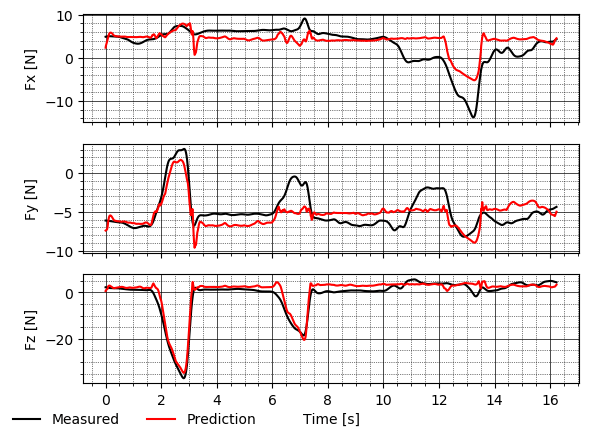
\includegraphics[width=0.495\columnwidth]{slike/Fig04_15a.png}}
    \hfil
    \subfloat[Arch. \#2\label{fig:Graph02}]{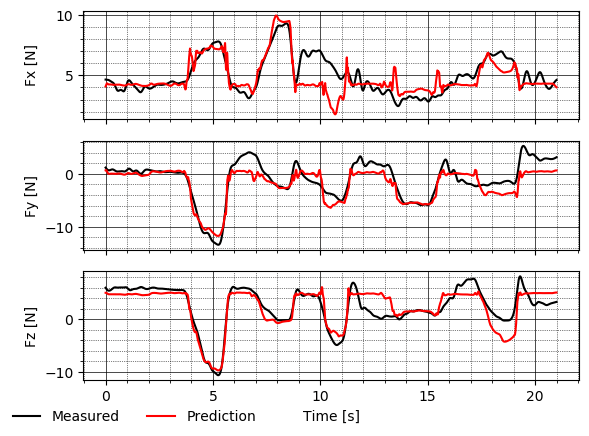
\includegraphics[width=0.495\columnwidth]{slike/Fig04_15b.png}}
    \vfil
    \subfloat[Arch. \#4\label{fig:Graph03}]{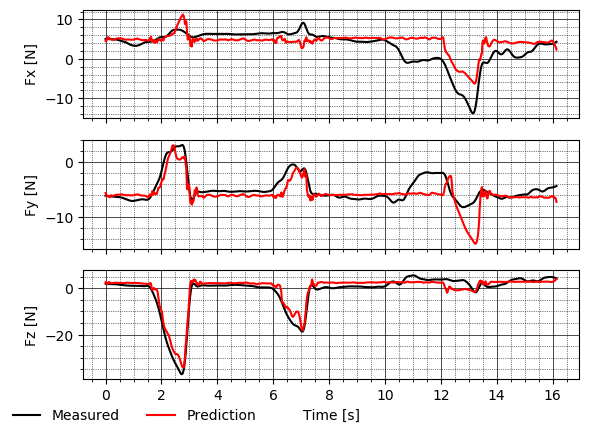
\includegraphics[width=0.495\columnwidth]{slike/Fig04_15c.png}}
    \hfil
    \subfloat[Arch. \#6\label{fig:Graph04}]{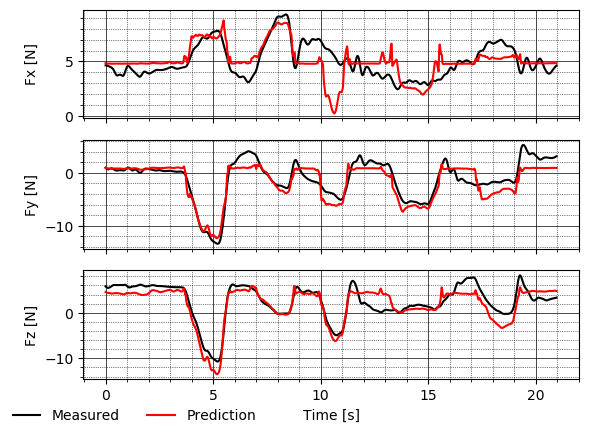
\includegraphics[width=0.495\columnwidth]{slike/Fig04_15d.png}}
    \vfil
    \subfloat[Arch. \#9\label{fig:Graph05}]{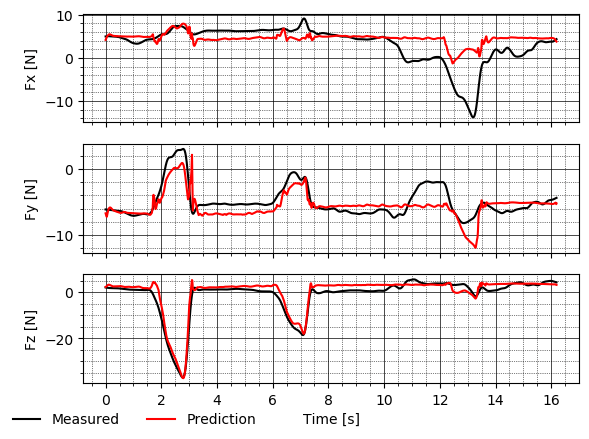
\includegraphics[width=0.495\columnwidth]{slike/Fig04_15e.png}}
    \hfil
    \subfloat[Arch. \#8\label{fig:Graph06}]{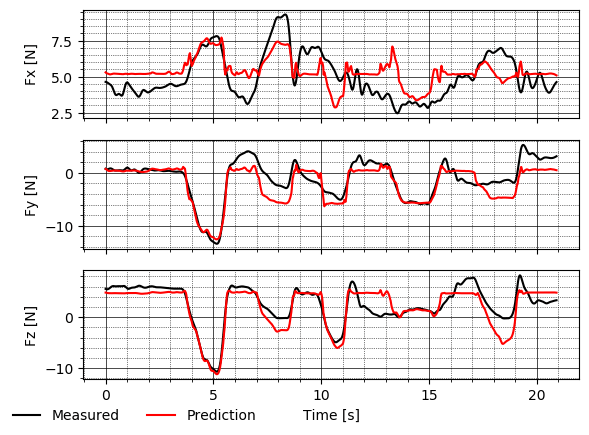
\includegraphics[width=0.495\columnwidth]{slike/Fig04_15f.png}}
    \caption{Example end-effector force predictions examples on test set for trained networks on Mover6 robot}
    \label{fig:Graphs}
\end{figure}

Obtained test results partly contain both ``good'' and ``bad'' predictions (i.e. in one part of a single test case, the predictions are good and in the other are not). Nevertheless, the general observation is that the obtained predictions suggest that multilayer perceptron architecture performs marginally worse than others and oscillate slightly more than the predictions made using the other two architectures. Moreover, by visual inspection of the obtained predictions shown in \cref{fig:Graphs}, it seems that they perform much worse than that the network test MAE suggests in Table \ref{tab:ResultsMover} suggest.

When looking at RMSE values obtained on the test set along each of the principal axes, it may be concluded that networks with a smaller number of total trainable parameters generally perform better (not depending on architecture). This observation is likely due to simple input data (i.e., a small number of features). Nevertheless, even using this metric, the best architecture is still a convolutional network by a small margin (the smallest in terms of the number of trainable parameters among those trained). In addition, on most trained networks, the RMSE value along the $z$ axis is the smallest one, which is encouraging because the force component along the $z$ axis is usually a dominant component of the force vector in the dataset used for training and testing. For example, for the architecture with the best obtained RMSE, 6 \% RMSE concerning the maximum force along the $z$ axis was achieved significantly better than 16 \% and 12 \% achieved along axes $x$ and $y$).

Based on these results, there is no clear-cut conclusion on which architecture is best for the task. However, architectures that consider input (measured) forces as time-series data have marginally better predictions. Please note that hyperparameter tuning for each of the architectures may provide somewhat better results. However, that would likely require a grid search approach to identify the optimal hyperparameters and a significant amount of time to train networks with all possible values of all chosen hyperparameters (i.e. the number of layers and the number of neurons per layers, activation function, optimiser, loss function).

The results for the neural networks trained using data obtained on the Franka robot in the simulation are shown in  Table \ref{tab:ResultsFranka} with row numbers corresponding to the architectures from Table \ref{tab:NetworksFranka}. 

From the results, it is apparent that the performance of the Franka robot is significantly better, i.e., that force estimates are much more accurate. Furthermore, unlike the Mover6 robot, which provides only joint positions, the Franka robot state is abundant with other features besides joint positions: joint velocities, accelerations and torques. Thus, more features to learn from are available, and the inverse dynamics of the Franka robot can be captured more accurately. Moreover, since joint velocities and accelerations are inputs of any inverse dynamics model, it makes the accurate learning of inverse dynamics possible. However, please note that inverse dynamics is learnt implicitly using our approach as part of an end-to-end neural network for end-effector force estimation.

\begin{table}
    \caption[Networks performance and RMSE metric for Franka robot (simulation)]{Network performance and RMSE metric for Franka robot in simulation}
    \label{tab:ResultsFranka}
    \centering
    \begin{tabular}{ccccc}
        \toprule
        \textbf{No.} & \textbf{Architecture} & \textbf{Validation Loss} & \textbf{Test Loss} & \textbf{RMSE} \\
        \midrule
        1 & MLP & 1.6544 & 1.6629 & 0.6871\\ % mlp_01
        2 & MLP &  0.9637 & 0.9513 & 0.5036\\ % mlp_03
        3 & MLP & 1.3130 & 1.2956 & 0.5440\\ % mlp_04
        4 & Conv & 1.1958 & 1.1644 & 0.4673\\ % conv_01
        5 & Conv & 1.3665 & 1.3101 & 0.5047\\ % conv_02
        6 & Conv & 0.9462 & 0.9535 & 0.4637\\ % conv_03
        7 & LSTM & 0.4790 & 0.4590 & 0.3204\\ % lstm_03
        8 & LSTM & 0.4868 & 0.4776 & 0.2740\\ % lstm_01
        9 & LSTM & 0.5422 & 0.5100 & 0.3224\\ % lstm_02
        \midrule
        10 $^*$ & LSTM & 0.1745 & 0.1690 & 0.1739 \\
        11 $^\dagger$ & LSTM & 0.1322 & 0.1189 & \textbf{0.1428}\\
        \bottomrule
        \multicolumn{5}{l}{\footnotesize{$^*$ Optimised architecture: three LSTM layers with 56, 48 and 16 cells, respectively }}\\
        \multicolumn{5}{l}{\footnotesize{$^\dagger$ Optimised architecture: two LSTM layers with 64 and 56 cells, respectively}}
    \end{tabular}
\end{table}

It is also noticeable from the obtained results that networks operating on sequential inputs perform better than multilayer perceptrons. However, contrary to \cref{tab:ResultsMover} for the Mover6 robot, LSTM networks have significantly better performance than convolutional (but, with the Mover6 robot, convolutional architectures had only marginally better performance). Moreover, including longer sequences of input data (five samples vs ten samples) improved performance. Finally, the inclusion of additional data about the robot state (this time those are joint torques) is also beneficial (as per RMSE metric) since it improved performance for each of the trained architectures compared with the performance of networks of the same architectures when those data were not used for about 15\%. Example force predictions from the test set using the trained networks are shown in \cref{fig:SimGraphs} (the architectures correspond to those defined in \cref{tab:NetworksFranka}.

\begin{figure}
    \centering
    \subfloat[MLP (arch. \#2)\label{fig:SimGraph01}]{
        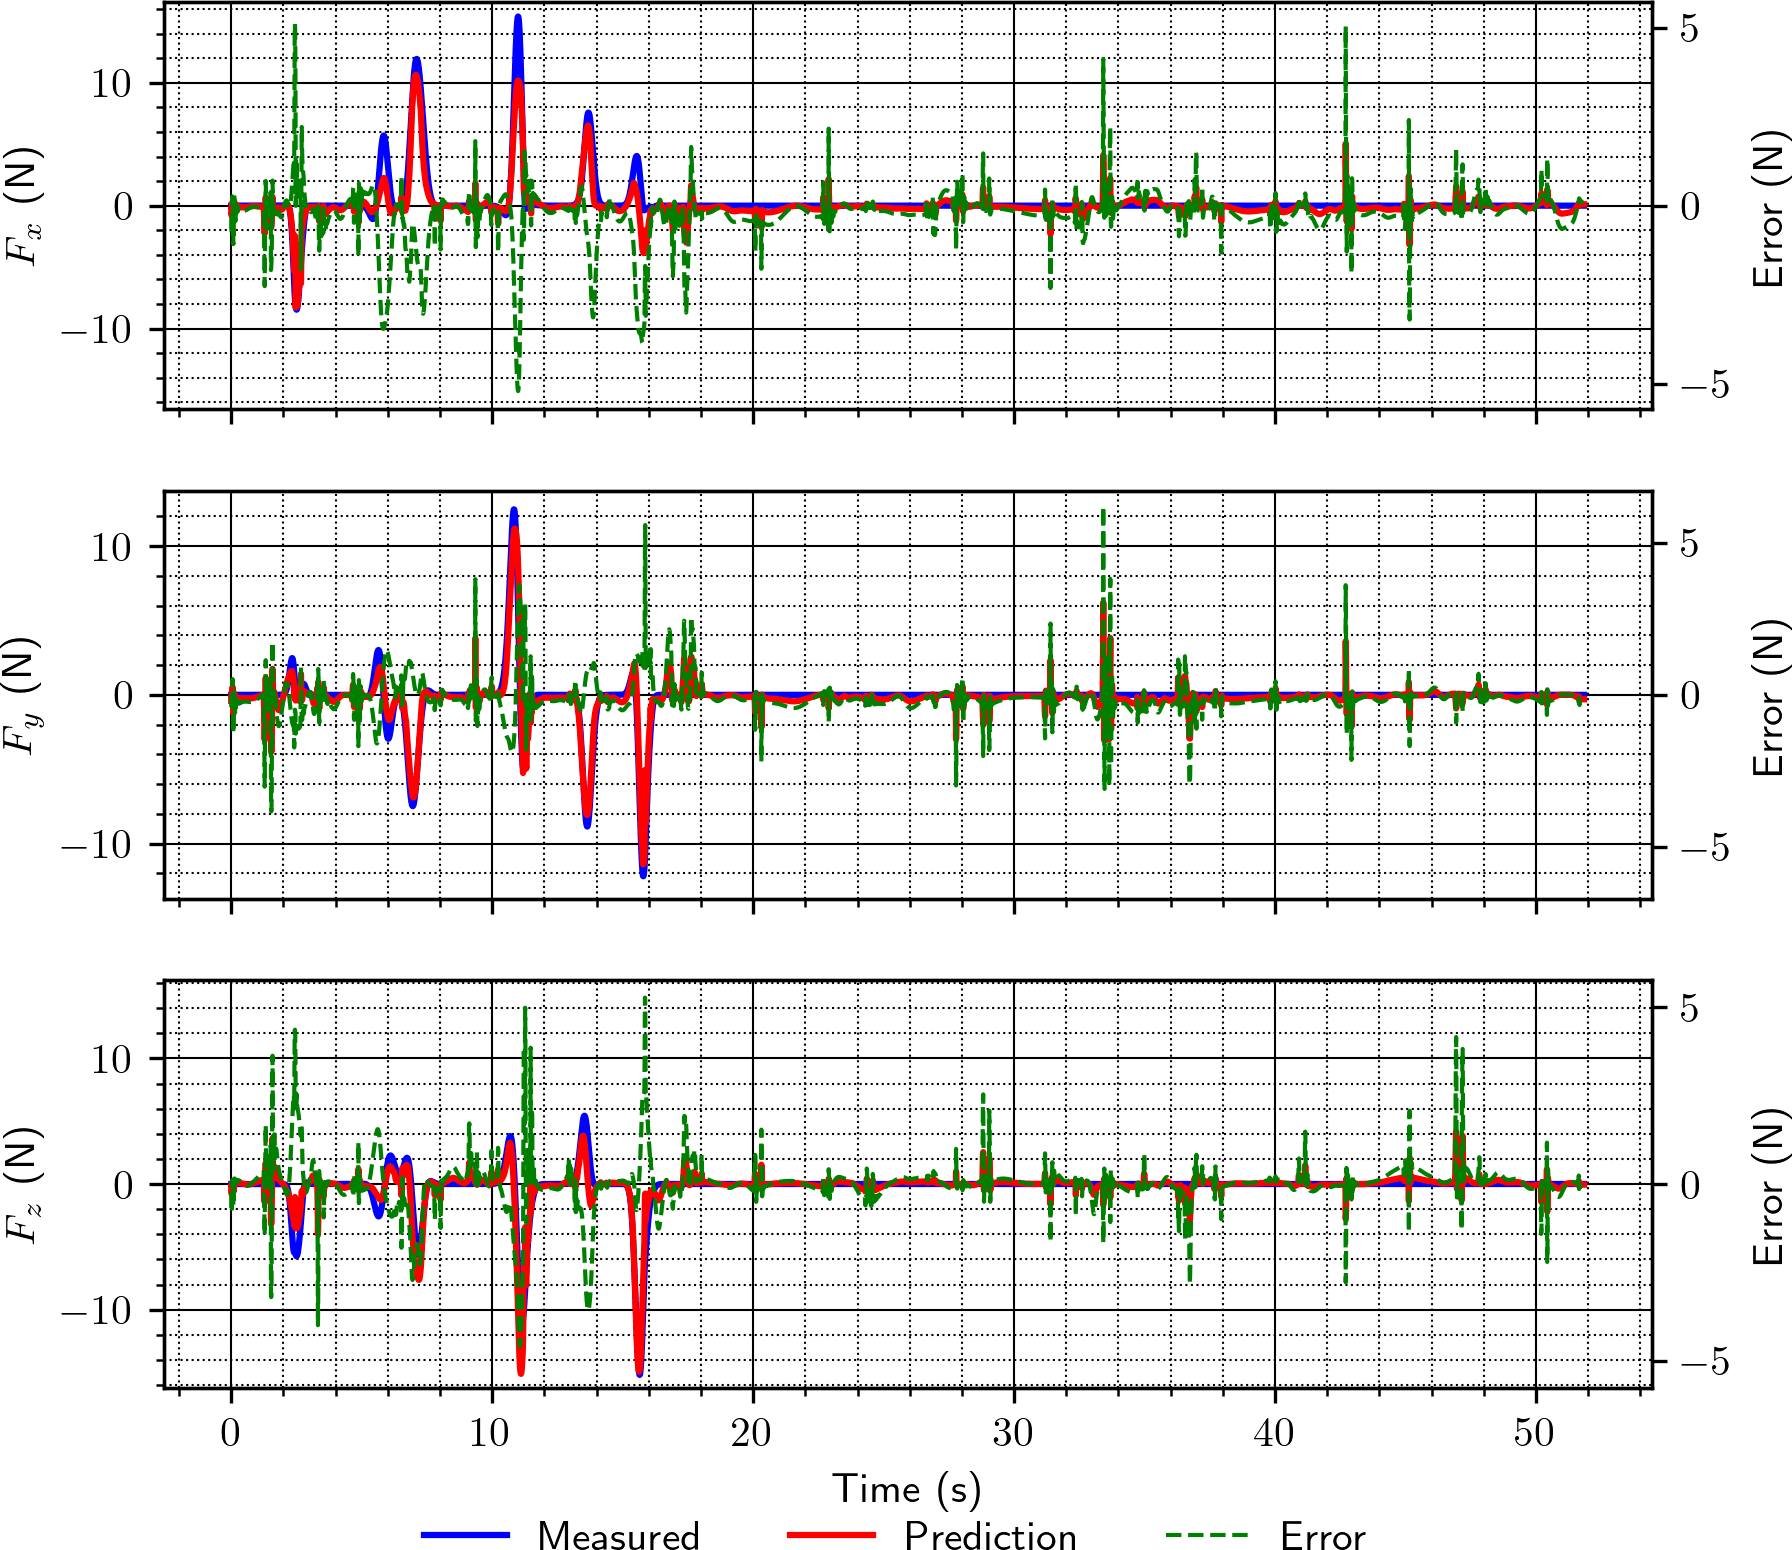
\includegraphics[width=0.48\textwidth]{slike/Fig04_16a.png}
    }
    \hfill
    \subfloat[MLP (arch. \#3)\label{fig:SimGraph02}]{
        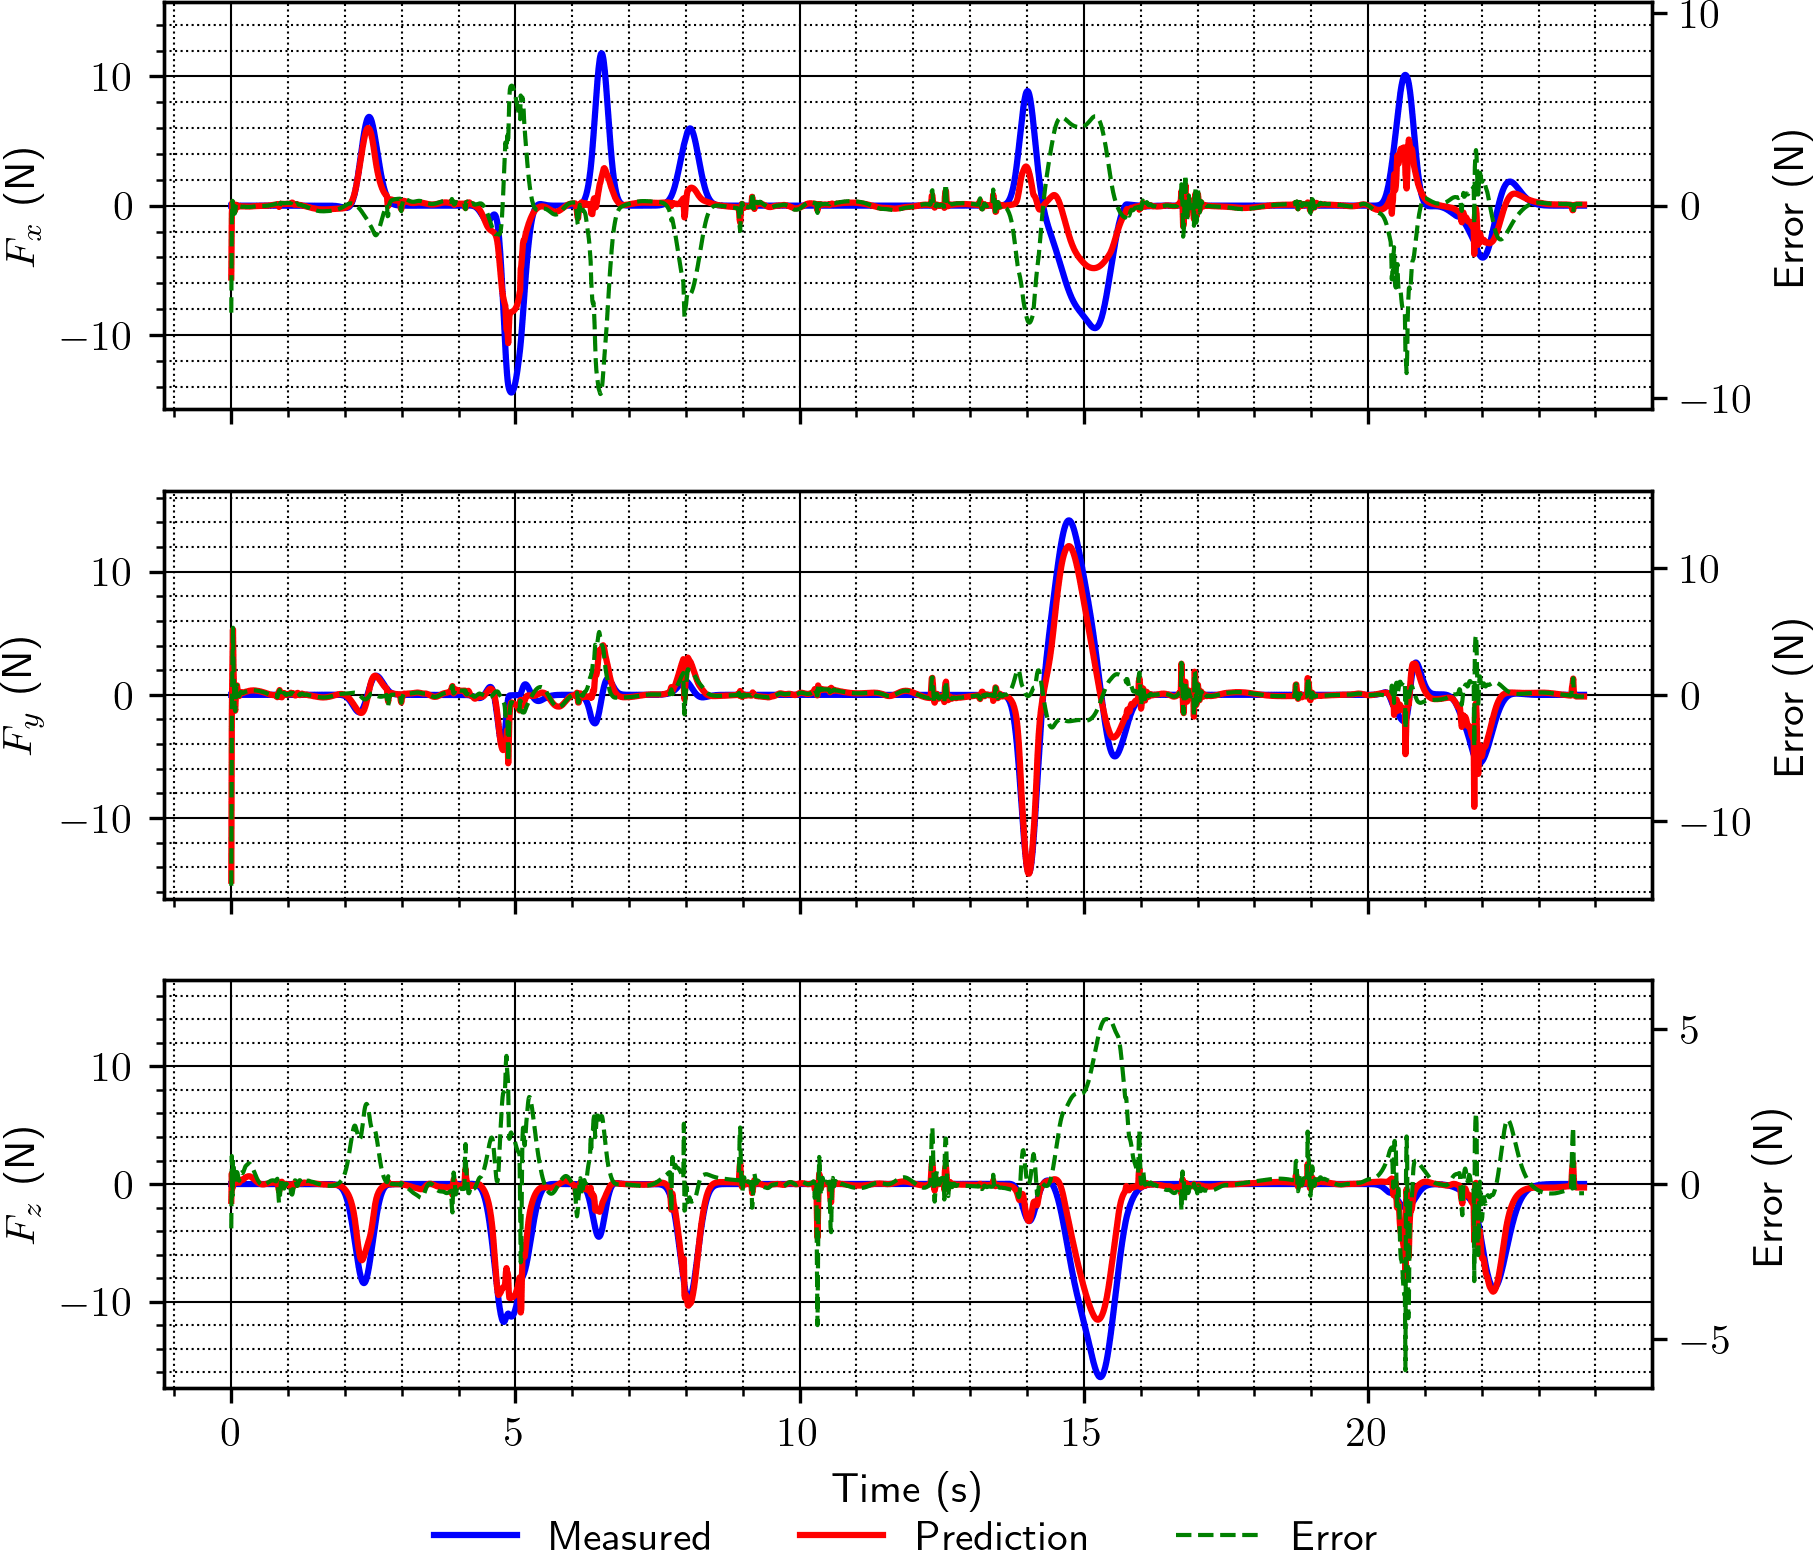
\includegraphics[width=0.48\textwidth]{slike/Fig04_16b.png}
    }
    \vfill
    \subfloat[Convolutional (arch. \#4)\label{fig:SimGraph03}]{
        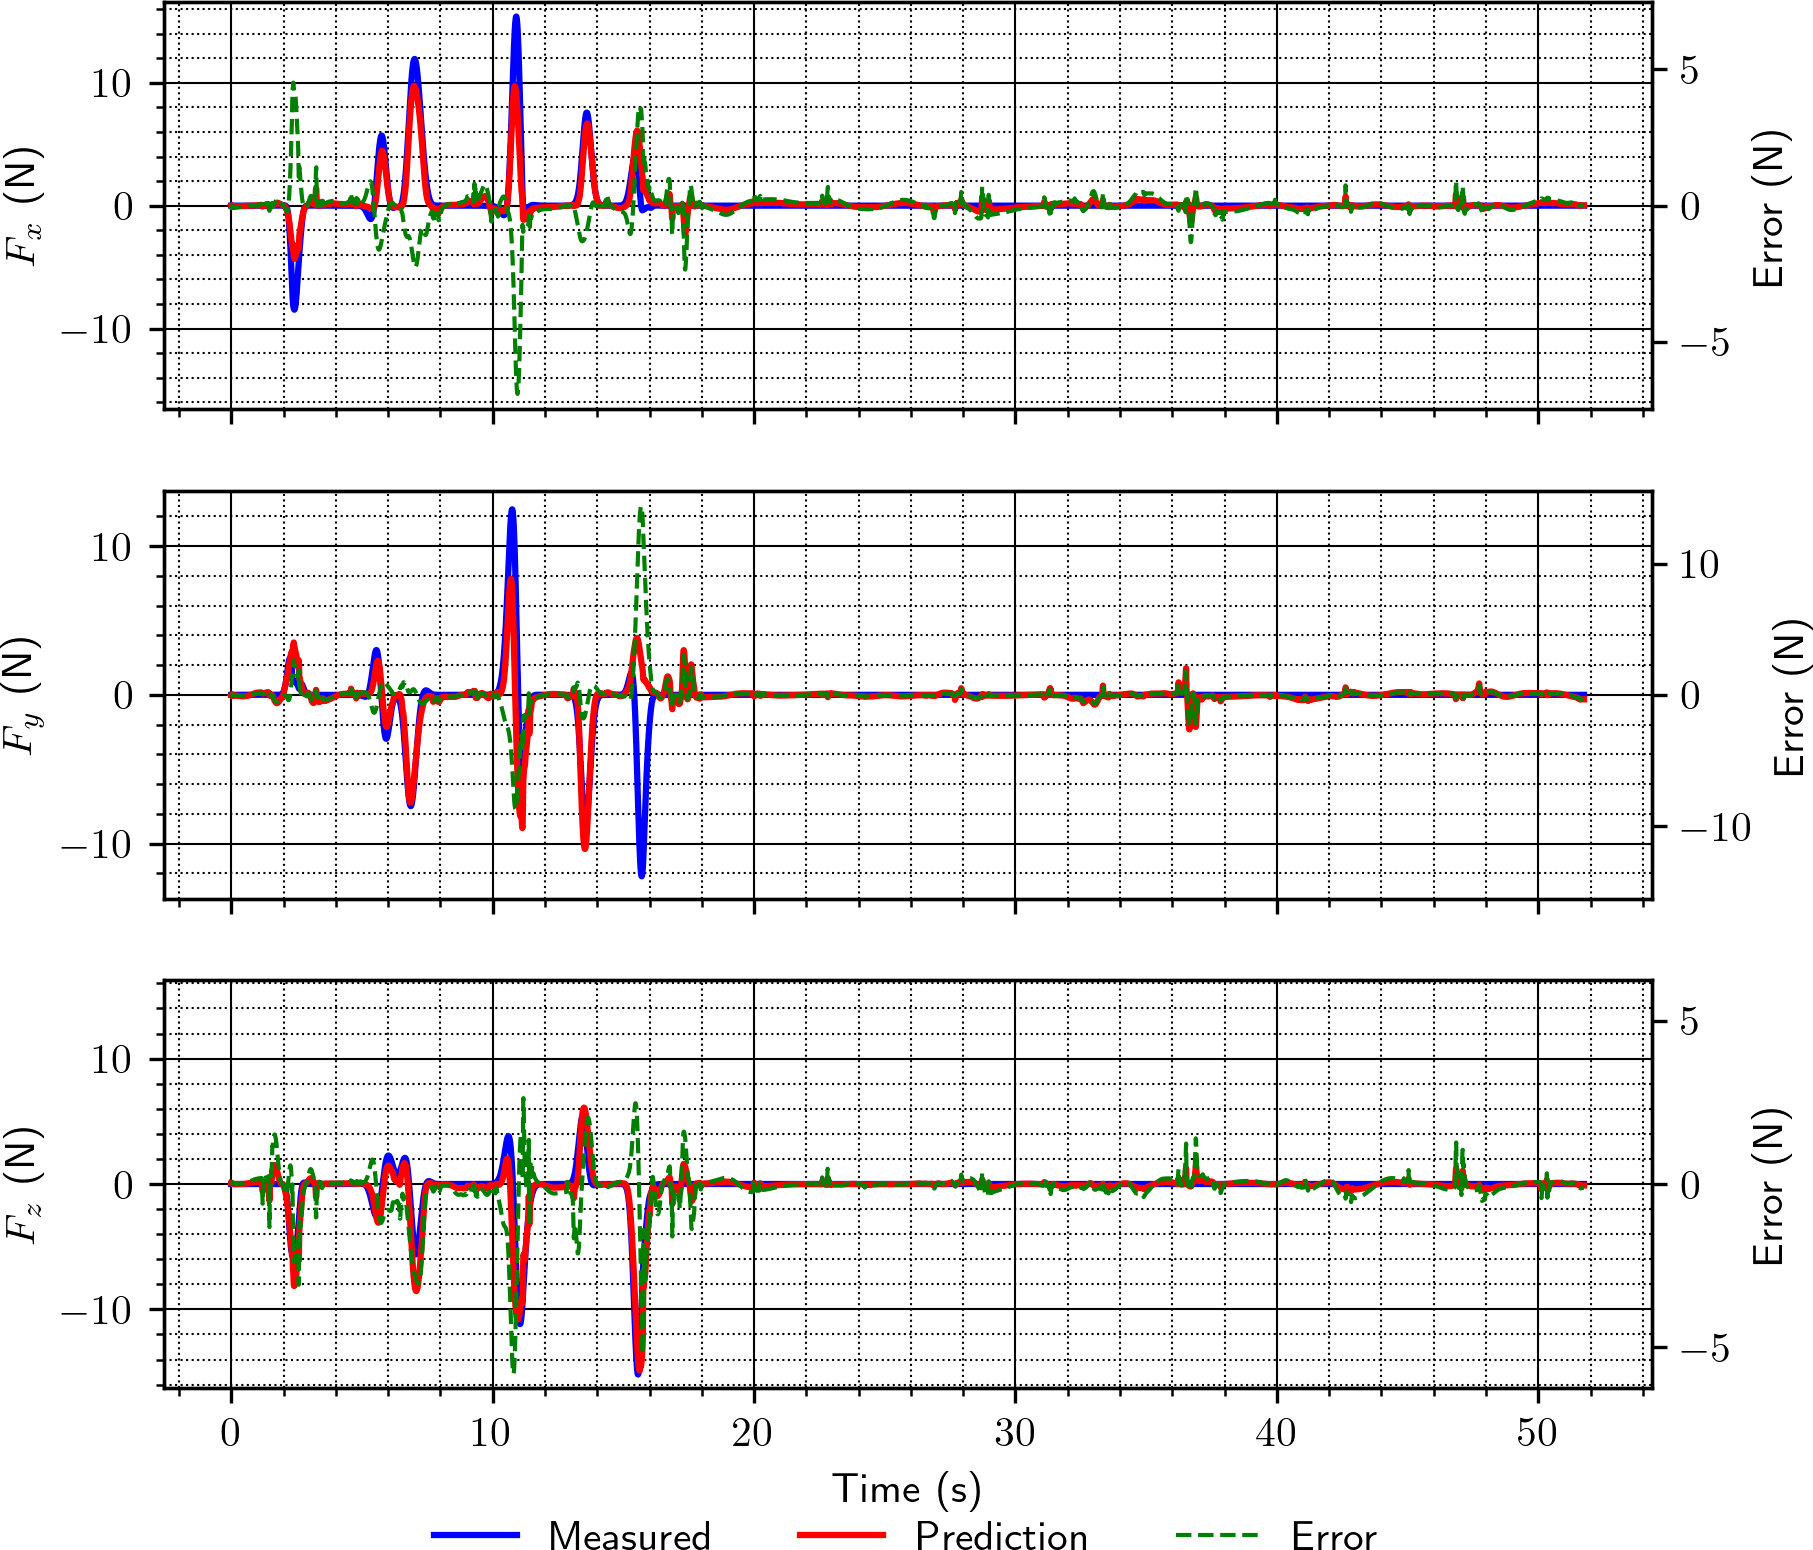
\includegraphics[width=0.48\textwidth]{slike/Fig04_16c.png}
    }
    \hfill
    \subfloat[Convolutional (arch. \#6)\label{fig:SimGraph04}]{
        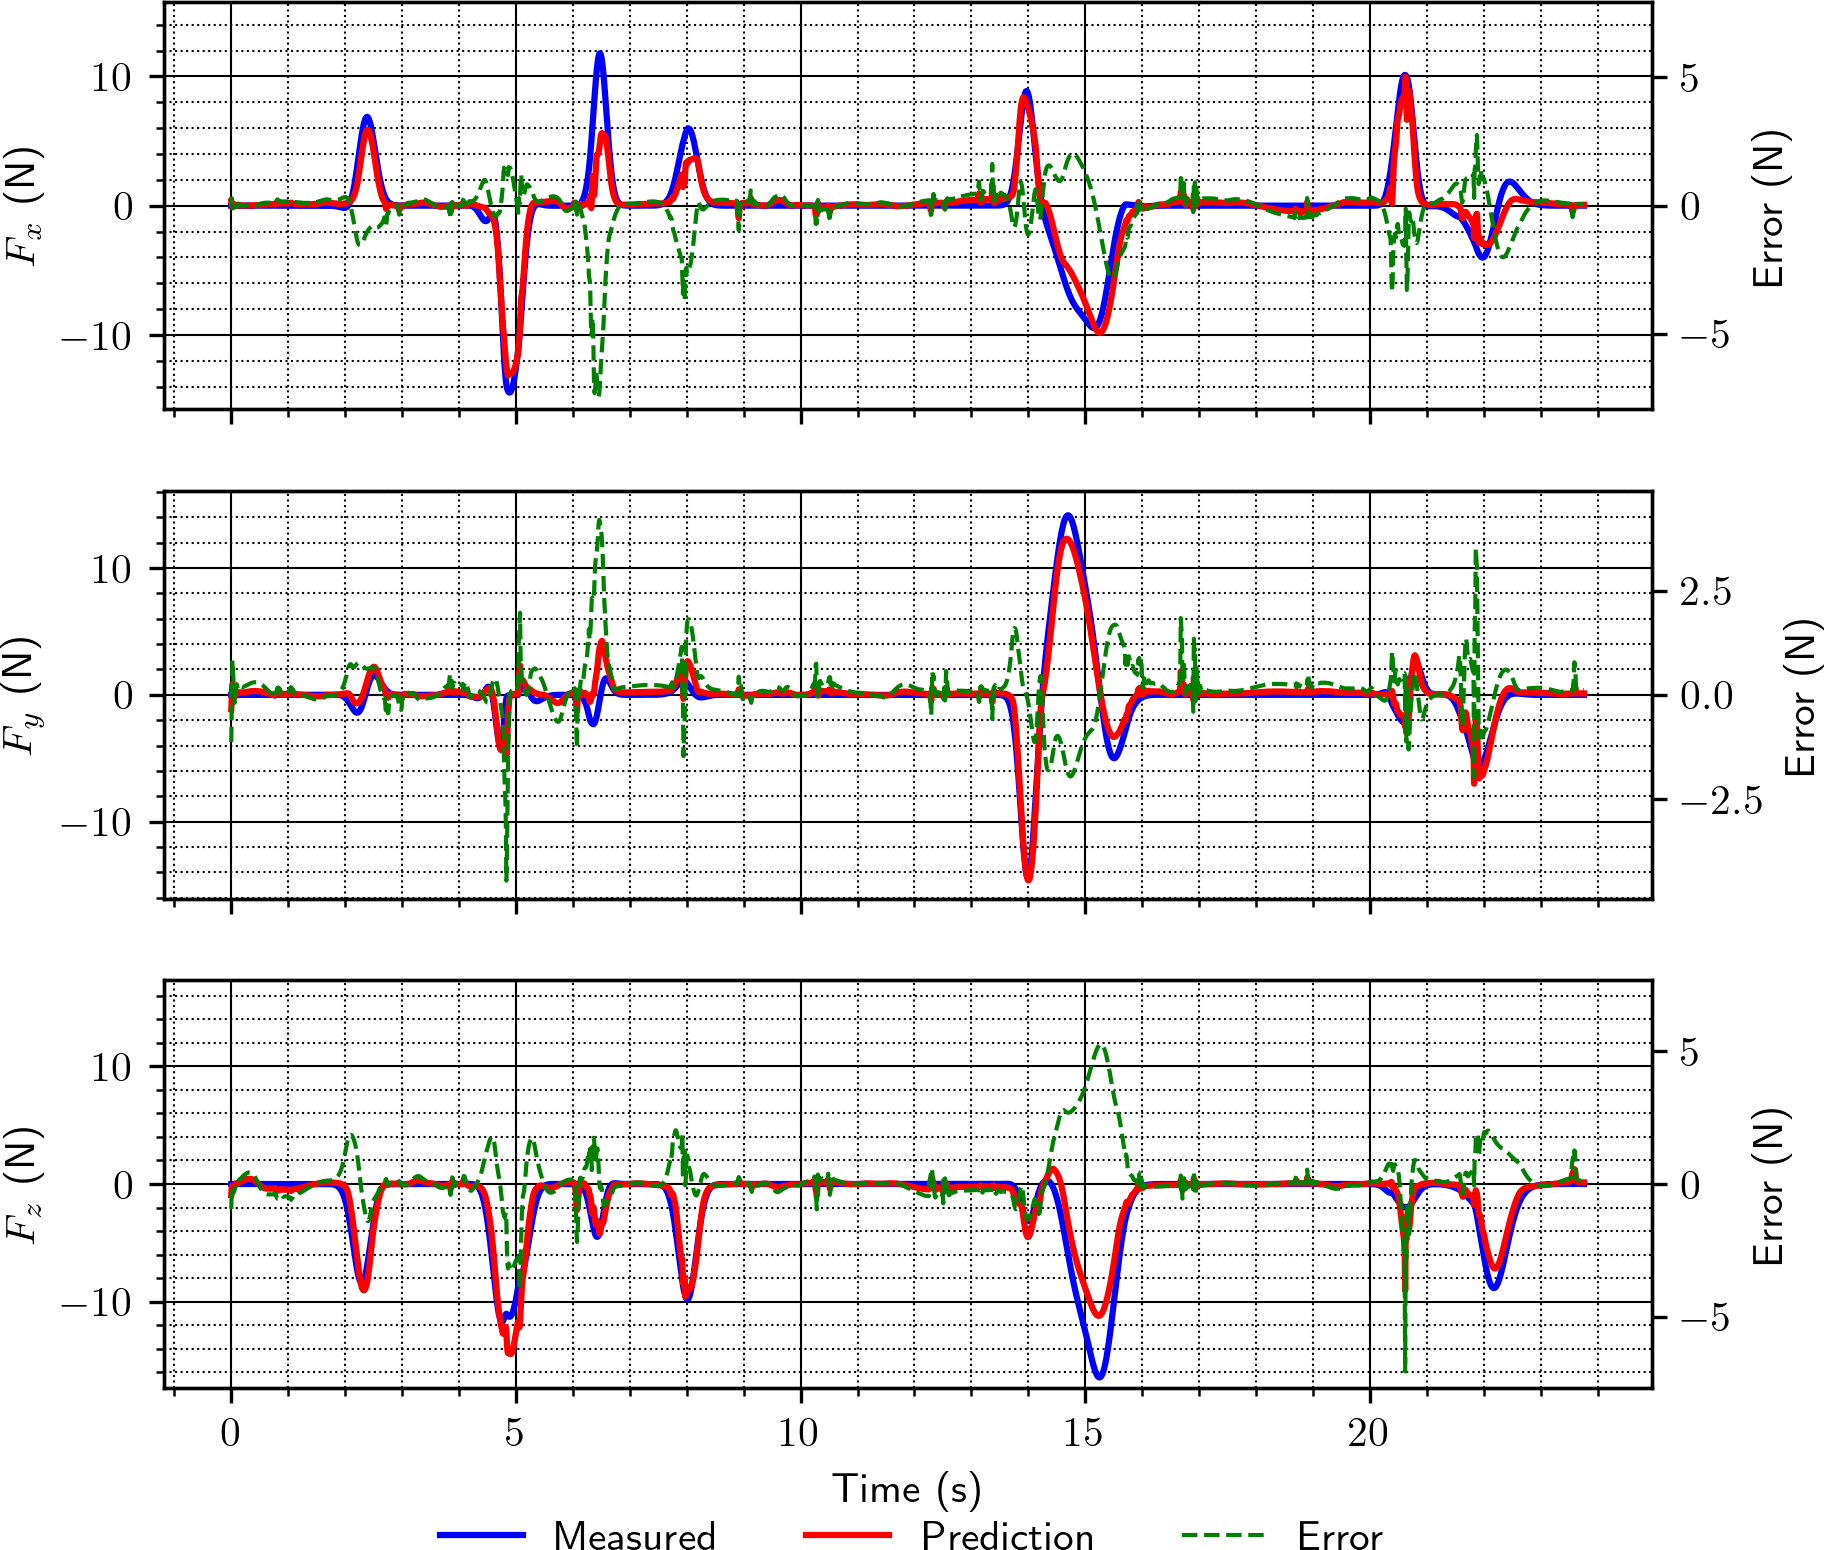
\includegraphics[width=0.48\textwidth]{slike/Fig04_16d.png}
    }
    \vfill
    \subfloat[LSTM (arch. \#7)\label{fig:SimGraph05}]{
        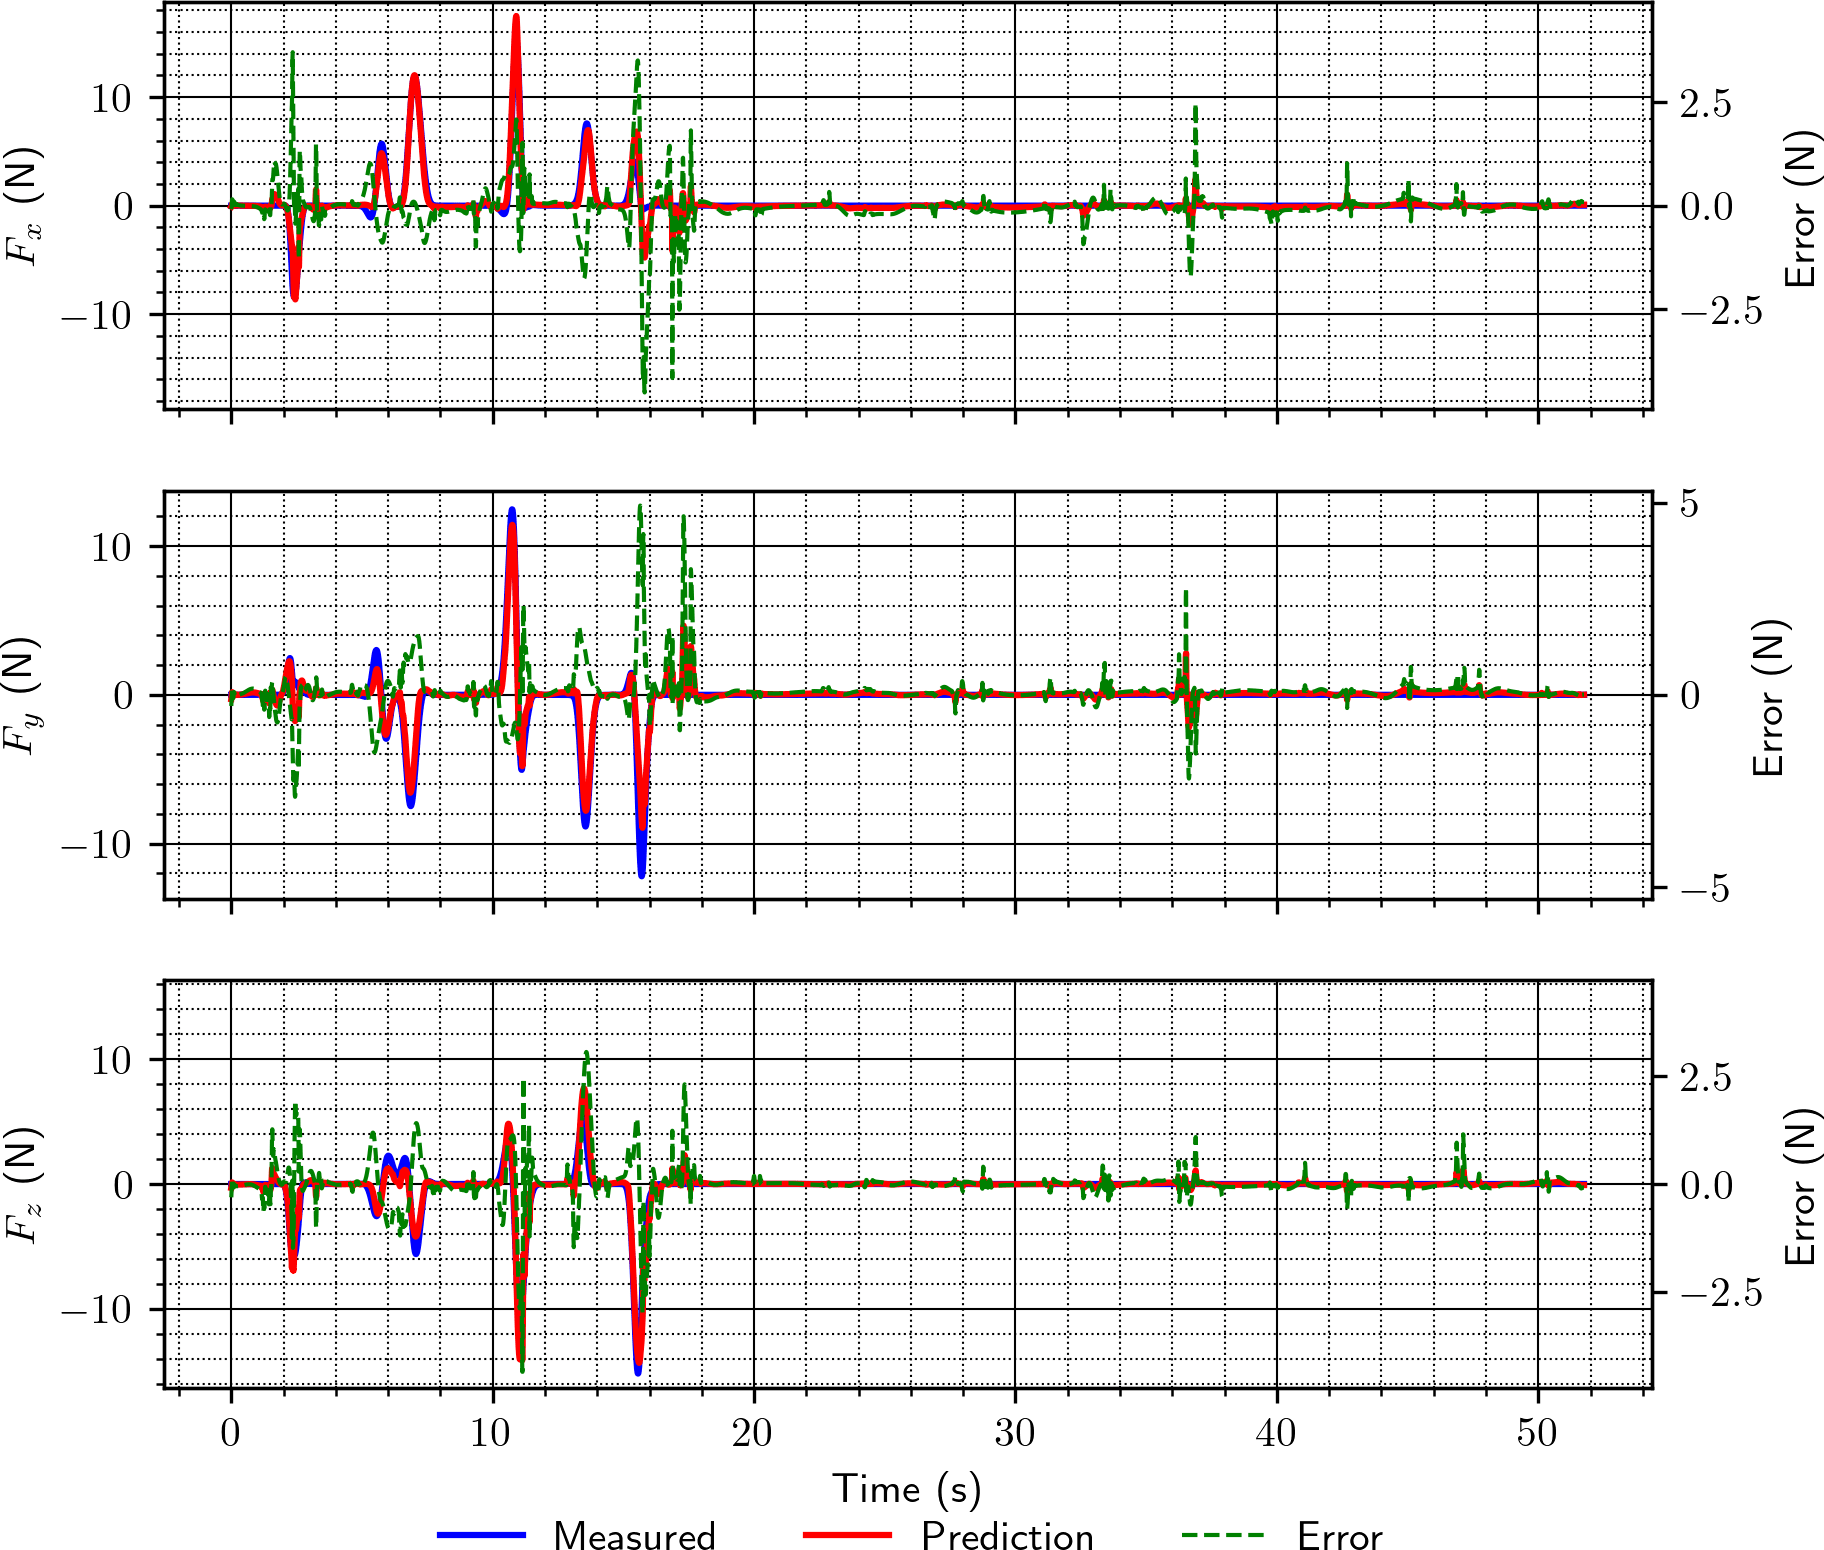
\includegraphics[width=0.48\textwidth]{slike/Fig04_16e.png}
    }
    \hfill
    \subfloat[LSTM (arch. \#9)\label{fig:SimGraph06}]{
        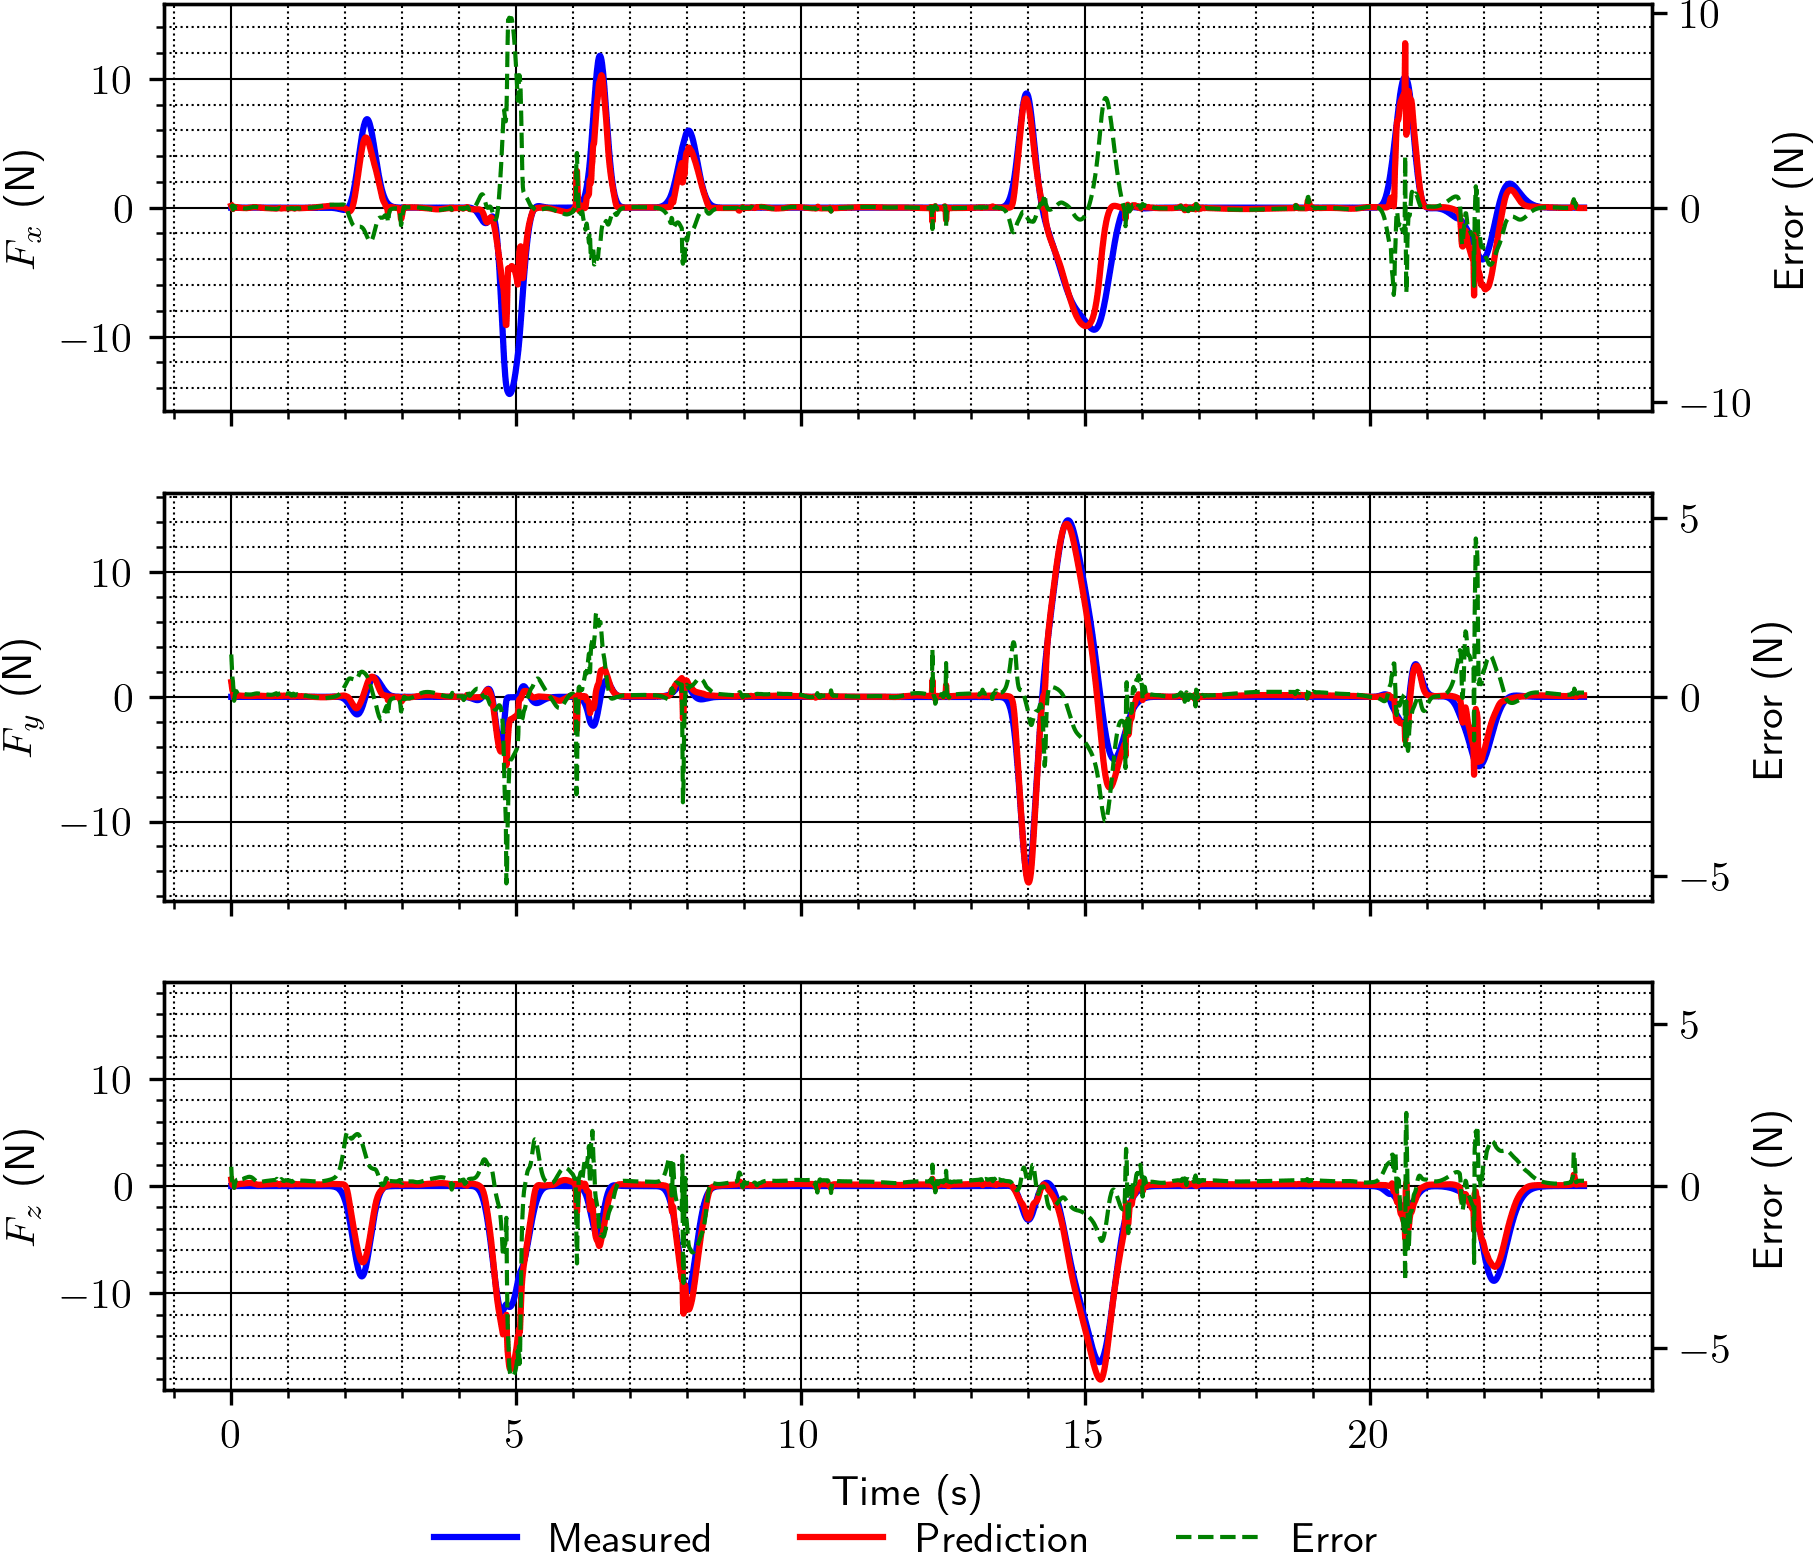
\includegraphics[width=0.48\textwidth]{slike/Fig04_16f.png}
    }
    \caption{End-effector force predictions examples on test set for trained networks on Franka robot in simulation}
    \label{fig:SimGraphs}
\end{figure}

The performed hyperparameter optimisation yielded networks that produced somewhat better estimates, at the cost of increased training time, due to the networks with larger number of trainable parameters. The example estimates are shown in \cref{fig:SimOptimEE}. The optimised network network that used a dataset with joint torques performed better than one without it, according to the RMSE (0.1428 vs 0.1739). Additionally, from the figure, it can be seen that estimates are better for all three axes and errors are smaller than with the presented networks that were not optimised.

\begin{figure}
    \centering
    \subfloat[Optimised LSTM (arch. \#10); Example 1]{
        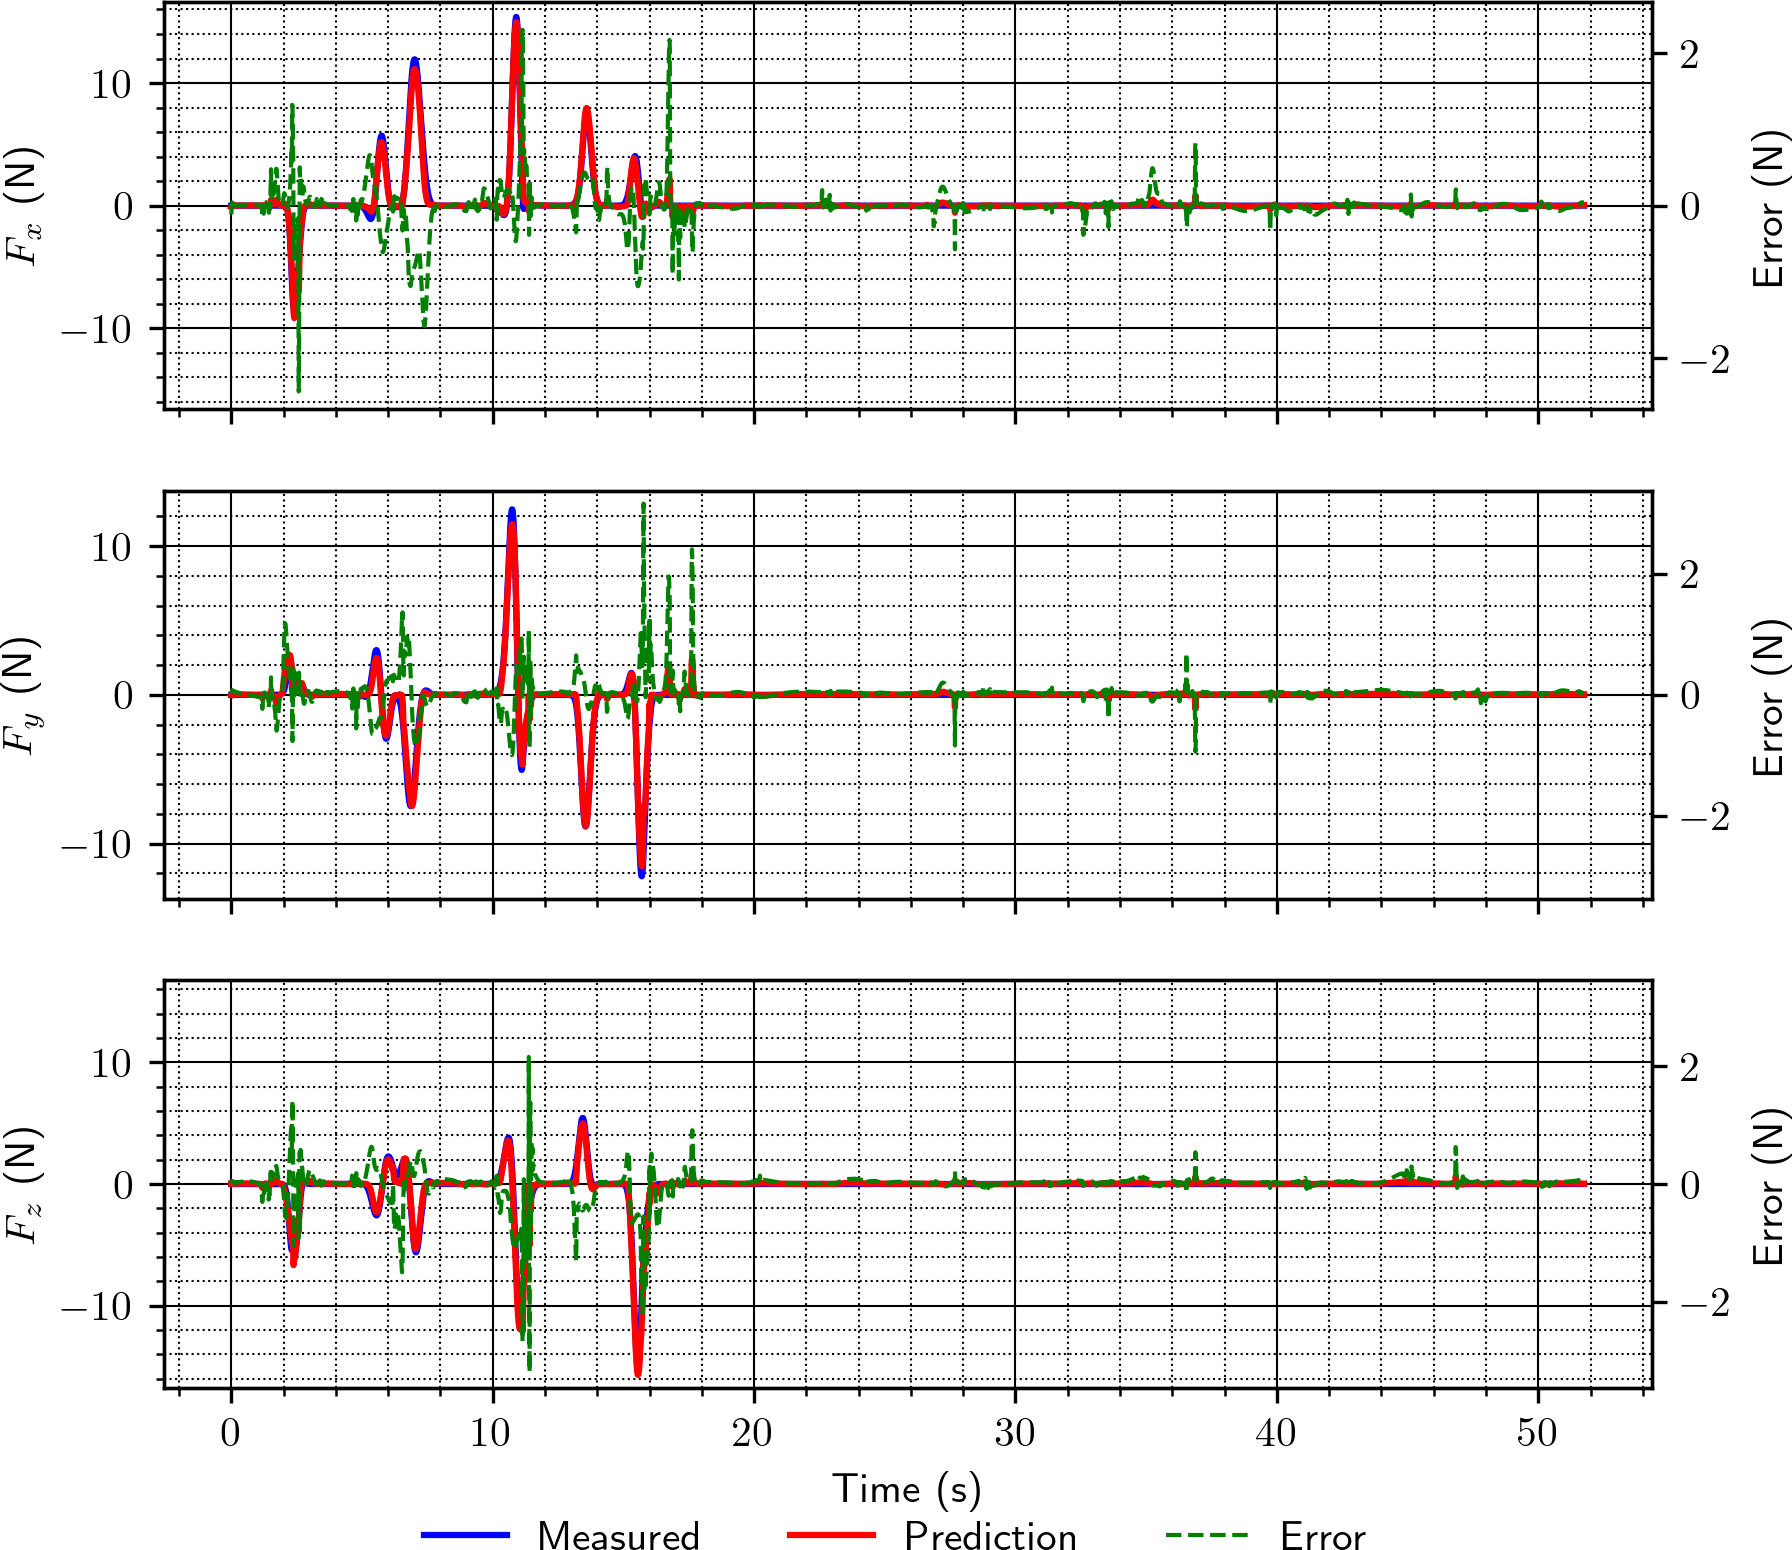
\includegraphics[width=0.48\textwidth]{slike/Fig04_17a.png}
    }
    \hfill
    \subfloat[Optimised LSTM (arch. \#10); Example 2]{
        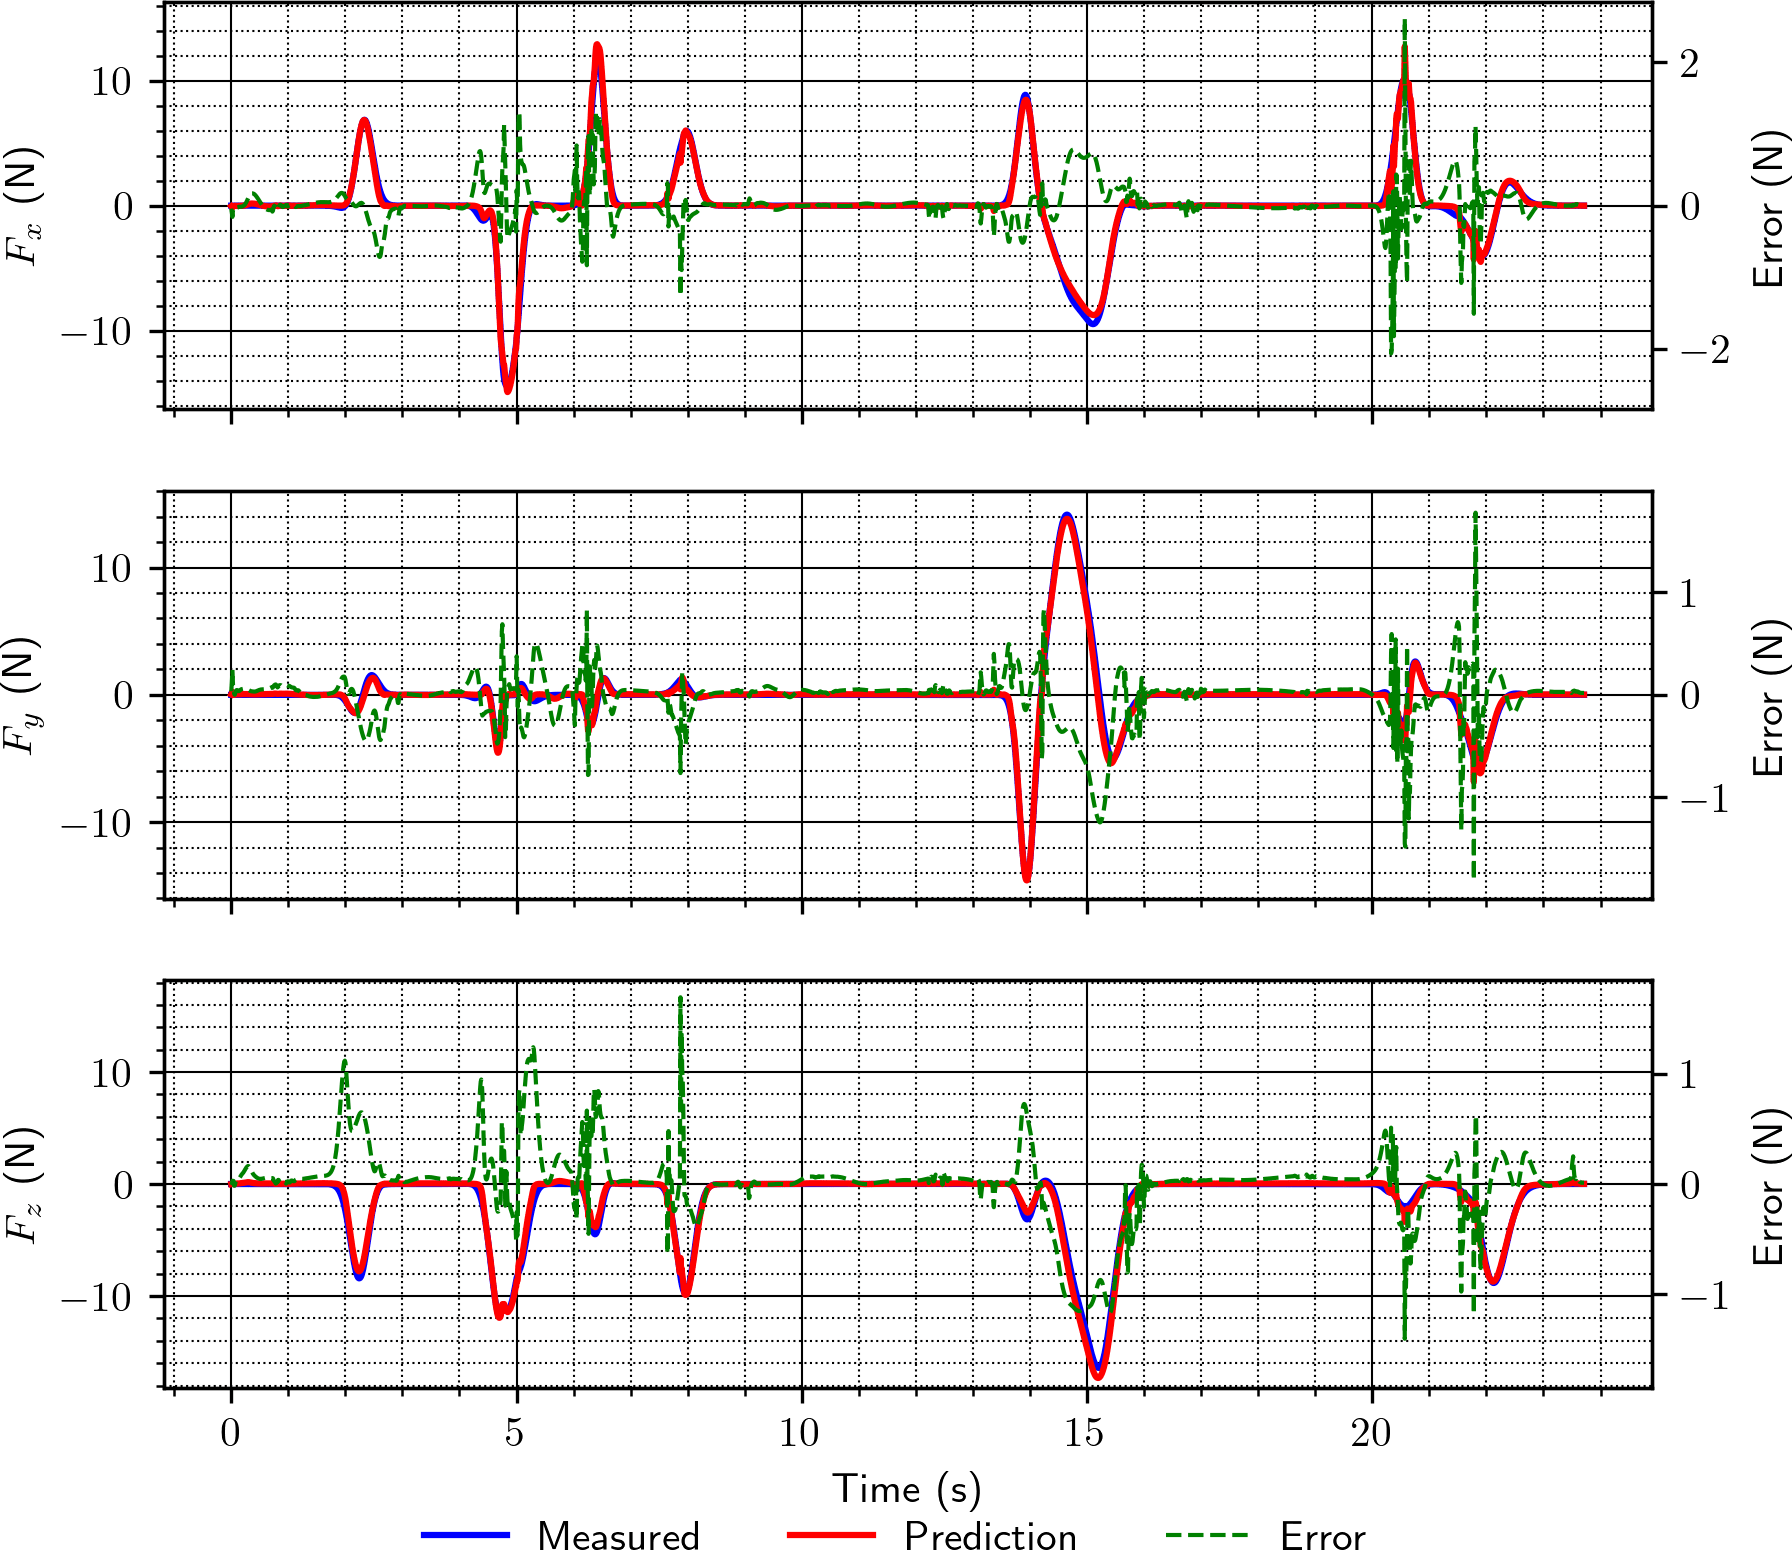
\includegraphics[width=0.48\textwidth]{slike/Fig04_17b.png}
    }
    \vfill
    \subfloat[Optimised LSTM (arch. \#11); Example 1]{
        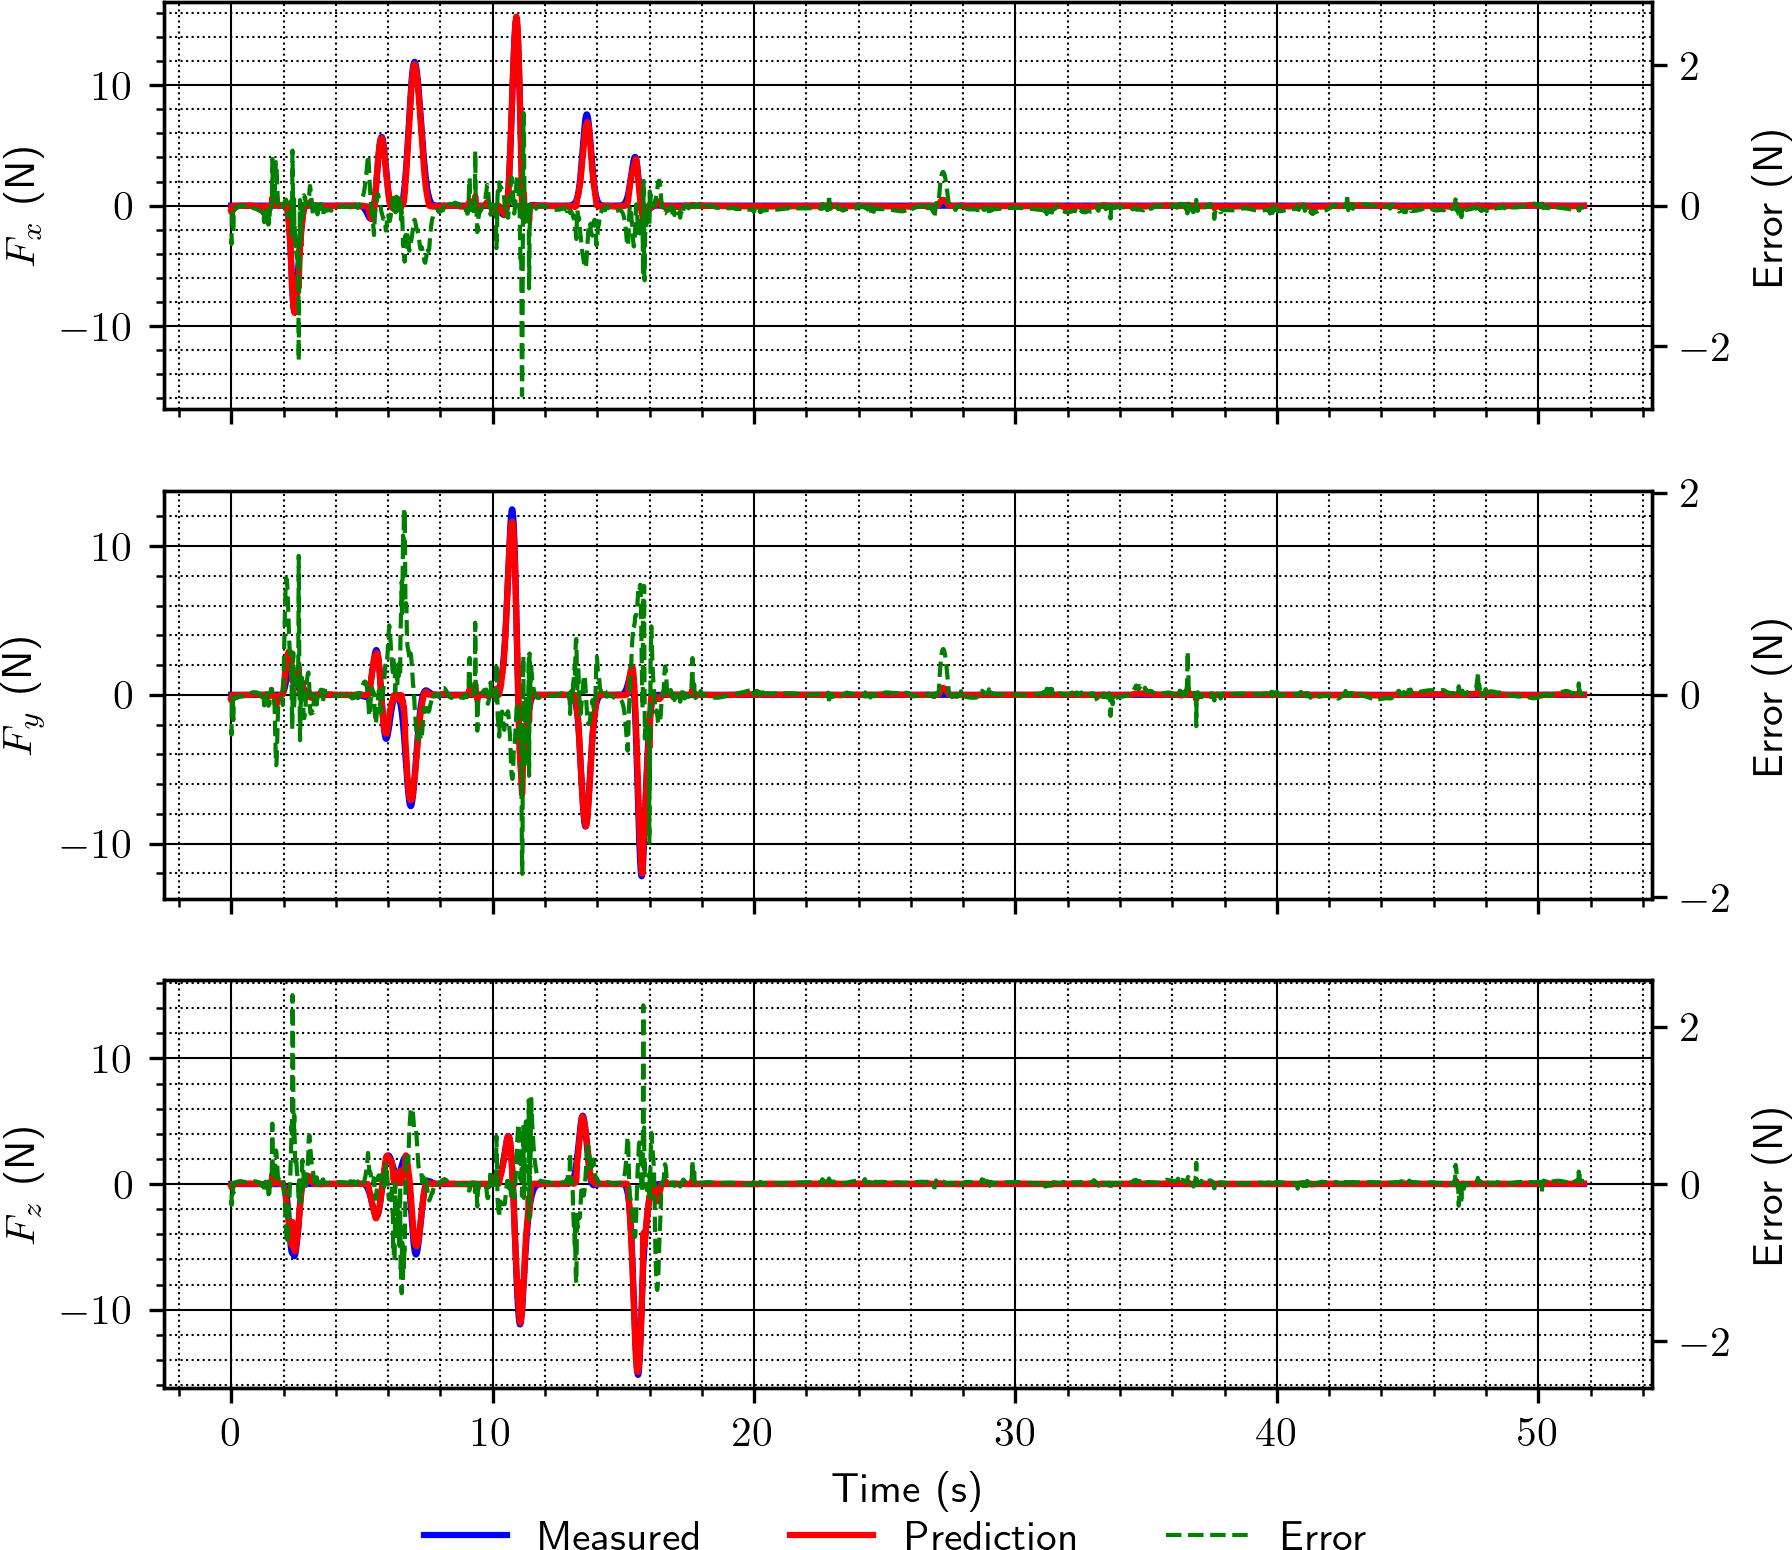
\includegraphics[width=0.48\textwidth]{slike/Fig04_17c.png}
    }
    \hfill
    \subfloat[Optimised LSTM (arch. \#11); Example 2]{
        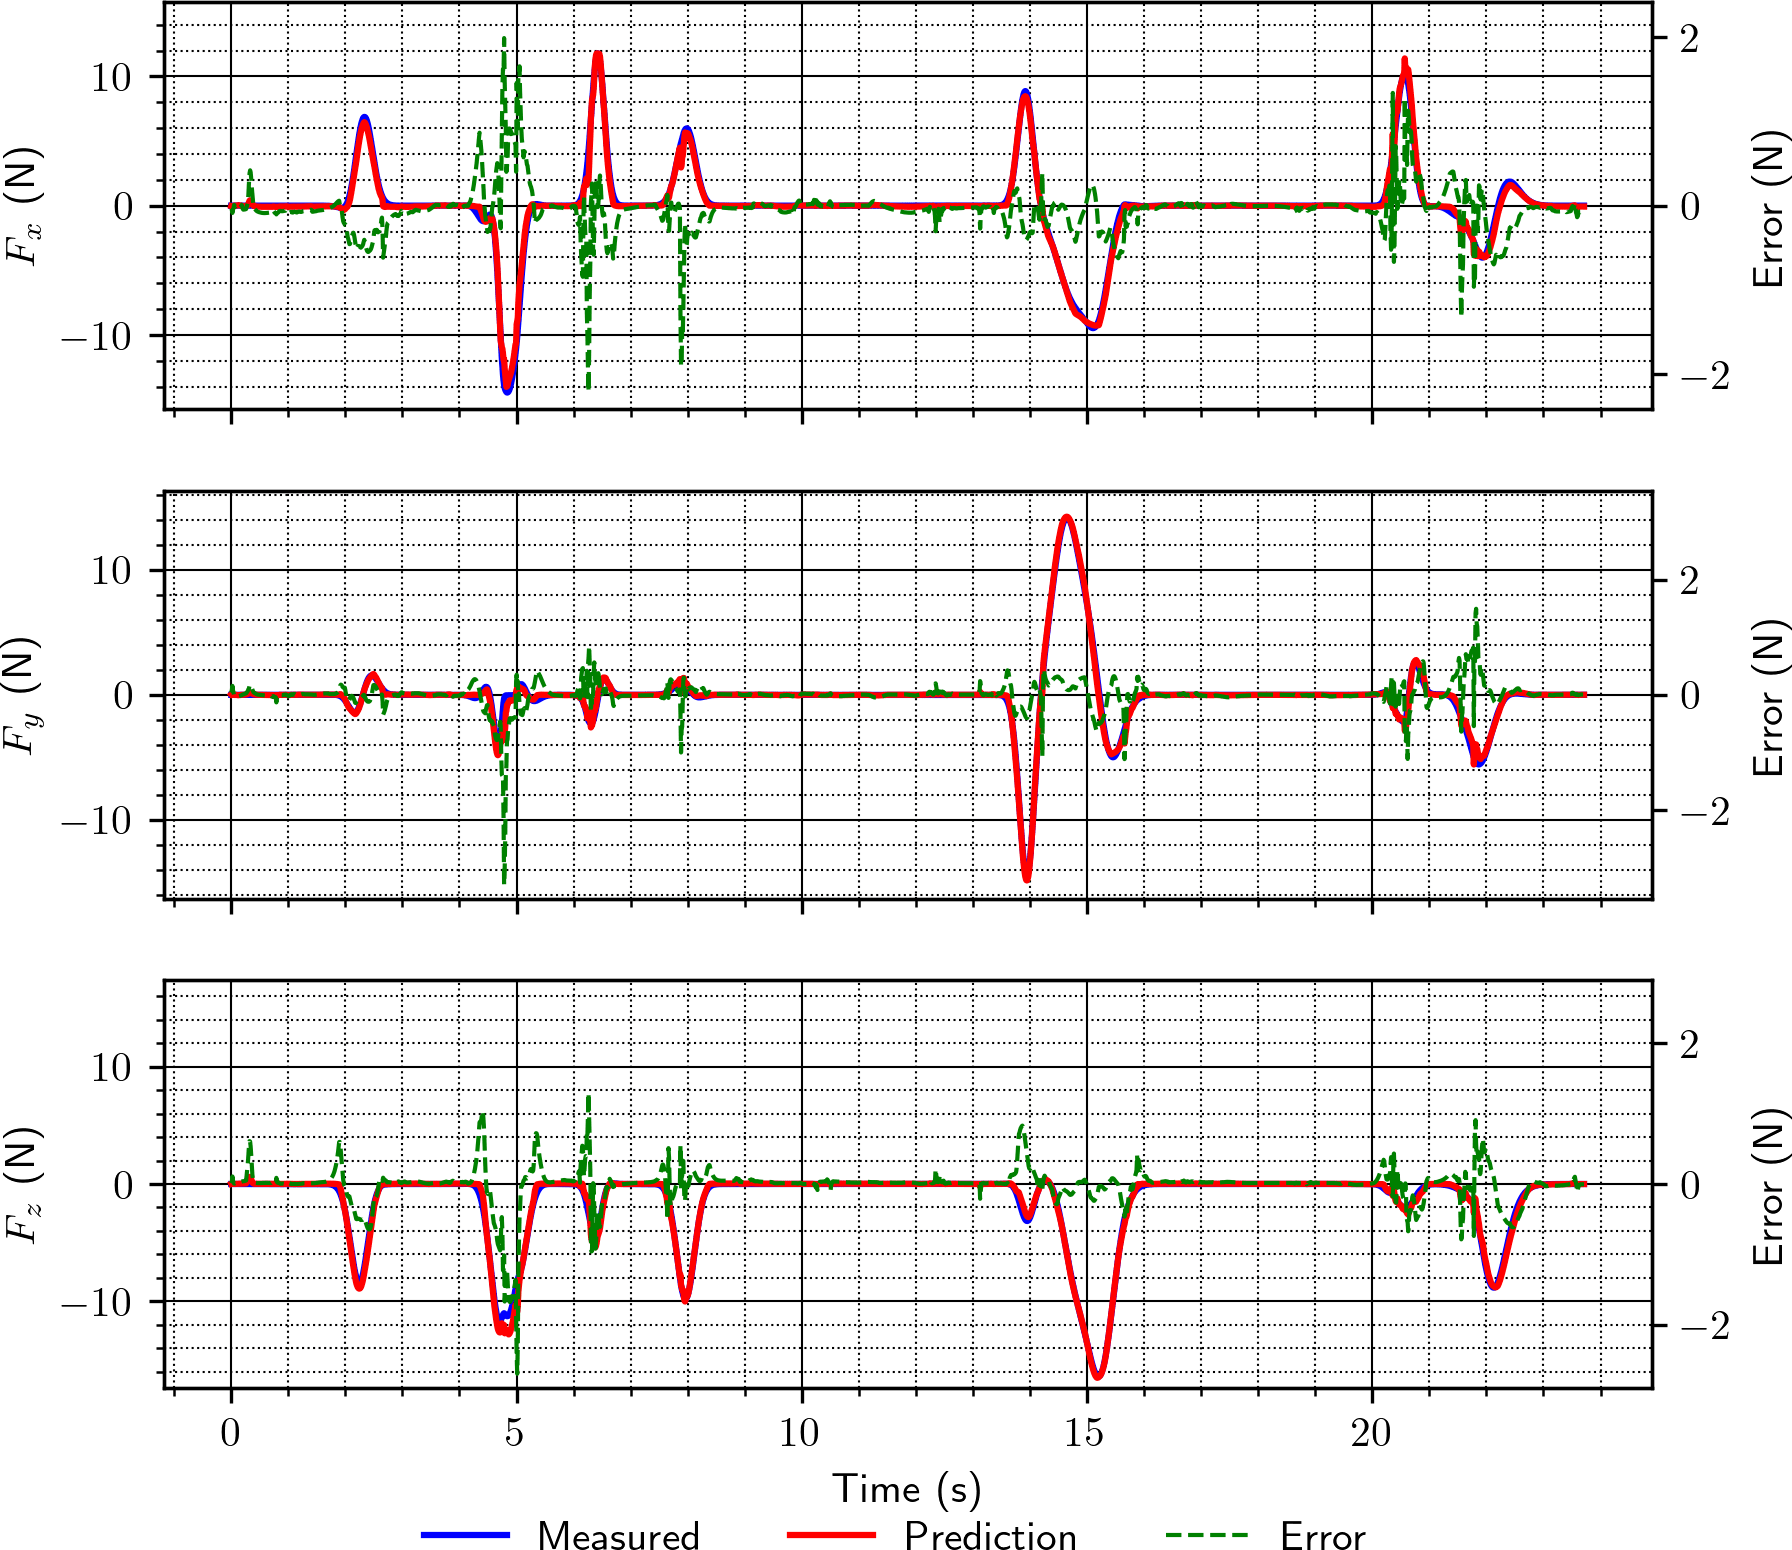
\includegraphics[width=0.48\textwidth]{slike/Fig04_17d.png}
    }
    \caption[Examples of end-effector force predictions using the simulation data on test set for optimised LSTM architectures]{Examples of end-effector force predictions using the simulation data on test set for optimised LSTM architectures (examples are corresponding to ones in \cref{fig:SimGraphs})}
    \label{fig:SimOptimEE}
\end{figure}

When comparing these results to Mover6 results, it is evident that Franka performs much better (evident both numerically in \cref{tab:ResultsFranka} and when comparing visually \cref{fig:Graphs,fig:SimGraphs}). This good performance might be because the data for training these networks were obtained in simulation, and the simulation is only an approximation of the real world, and it is expected that the simulation performs better than the real-world robot. Moreover, the Franka robot provides more information regarding the robot state (joint positions, velocities and torques vs joint positions only with Mover6 robot), and thus there are more features to train on, and consequently, the networks generalise better.

\begin{table}
    \caption[Network fitness and RMSE metric for Franka robot (real world)]{Network fitness and RMSE metric for Franka robot in real world}
    \label{tab:ResultsFrankaReal}
    \centering
    \begin{tabular}{ccccc}
        \toprule
        \textbf{No.} & \textbf{Architecture} & \textbf{Validation Loss} & \textbf{Test Loss} & \textbf{RMSE} \\
        \midrule
        1 & MLP & 6.0652 & 5.8790 & 1.3691 \\ % mlp_04
        2 & MLP & 6.9703 & 6.9400 & 1.5304   \\ % mlp_05
        3 & MLP & 6.4415 & 6.4206 & 1.5008 \\ % mlp_06
        4 & Conv & 6.3967 & 6.5539 & 1.3432 \\ % conv_01
        5 & Conv & 6.1087 & 6.2422 & \textbf{1.3203} \\ % conv_02
        6 & Conv & 6.7443 & 6.4727 & 1.4648 \\ % conv_03
        7 & LSTM & 7.2168 & 6.9944 & 1.3963 \\ % lstm_01
        8 & LSTM & 7.5325 & 7.5721 & 1.5971 \\ % lstm_02
        9 & LSTM & 7.8321 & 7.7343 & 1.6111 \\ % lstm_03
        \bottomrule
    \end{tabular}
\end{table}

Similarly to the networks trained on simulation data, the networks were trained with data obtained using the real Franka robot, with the same architectures with the results reported in Table \ref{tab:ResultsFrankaReal} (again, with rows corresponding to ones from \cref{tab:NetworksFranka}). However, from the results, it is clear that the performance the networks show is significantly worse than one of those trained using simulation data (shown in Table \ref{tab:ResultsFranka}, and even worse than that of Mover6 real robot). Furthermore, the trained networks seem not to generalise appropriately, i.e., validation loss is significantly higher than training loss and with training and validation loss during the training highly diverging, as shown in Figure \ref{fig:HistSimVsReal}. The mentioned reasons led to the conclusion that there is something wrong with the data: training and validation set data do not come from the same distribution. These high losses, in turn, translate to highly inaccurate predictions on the test set, as is shown on selected examples in Figure \ref{fig:RealGraphs}. Please also note that, besides the wrong amplitudes and shapes of (parts of) signal predictions, the sign of the force components is often mispredicted. 

\begin{figure}
    \centering
    \subfloat[Simulation data]{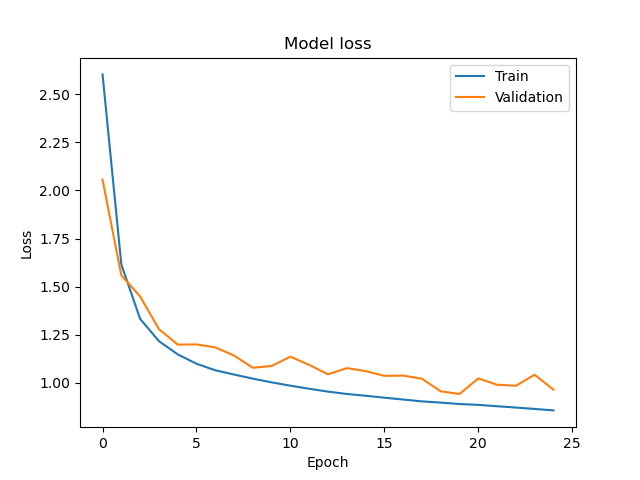
\includegraphics[width=0.495\textwidth]{slike/Fig04_18a.png}}
    \hfill
    \subfloat[Real-world data]{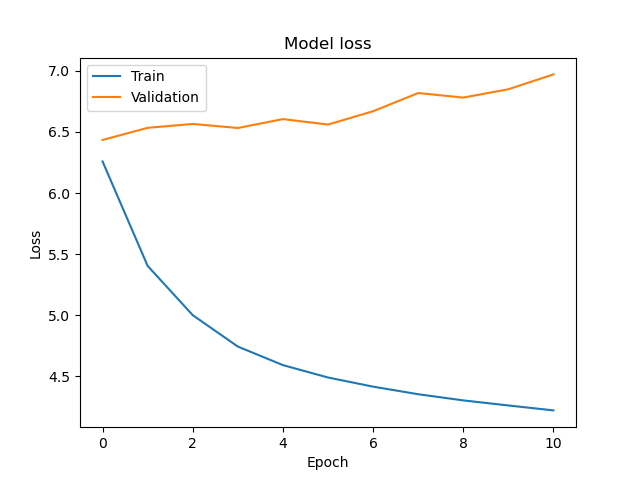
\includegraphics[width=0.495\textwidth]{slike/Fig04_18b.png}}
    \caption{Training vs. validation loss comparison between simulated and real-world Franka robot}
    \label{fig:HistSimVsReal}
\end{figure}

\begin{figure}
    \centering
    \subfloat[MLP (arch. \#1)]{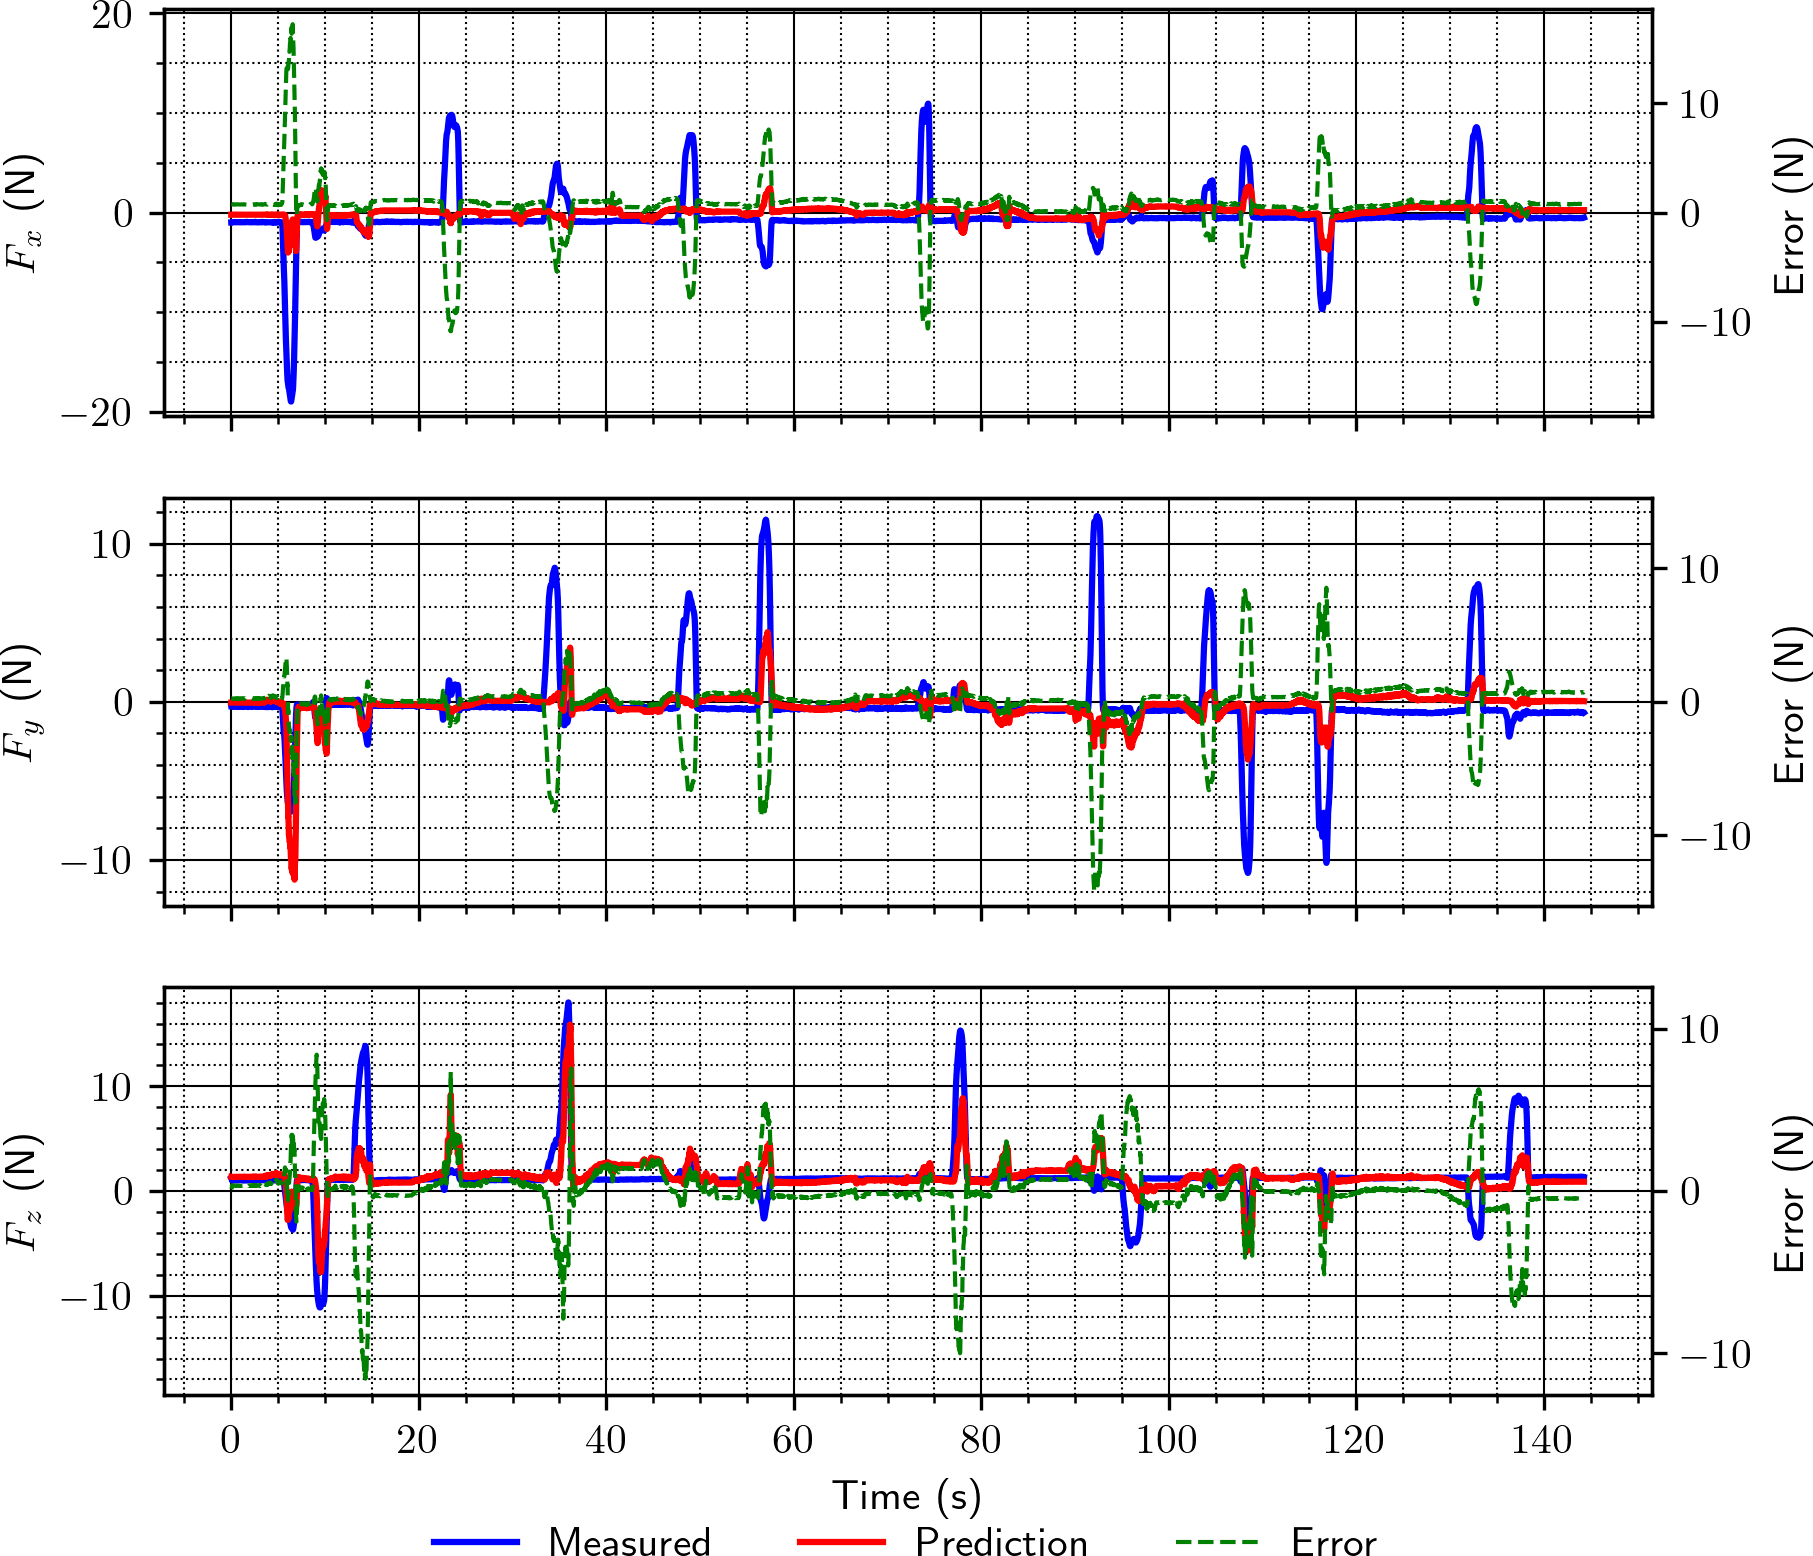
\includegraphics[width=0.48\columnwidth]{slike/Fig04_19a.png}}
    \hfil
    \subfloat[MLP (arch. \#2)]{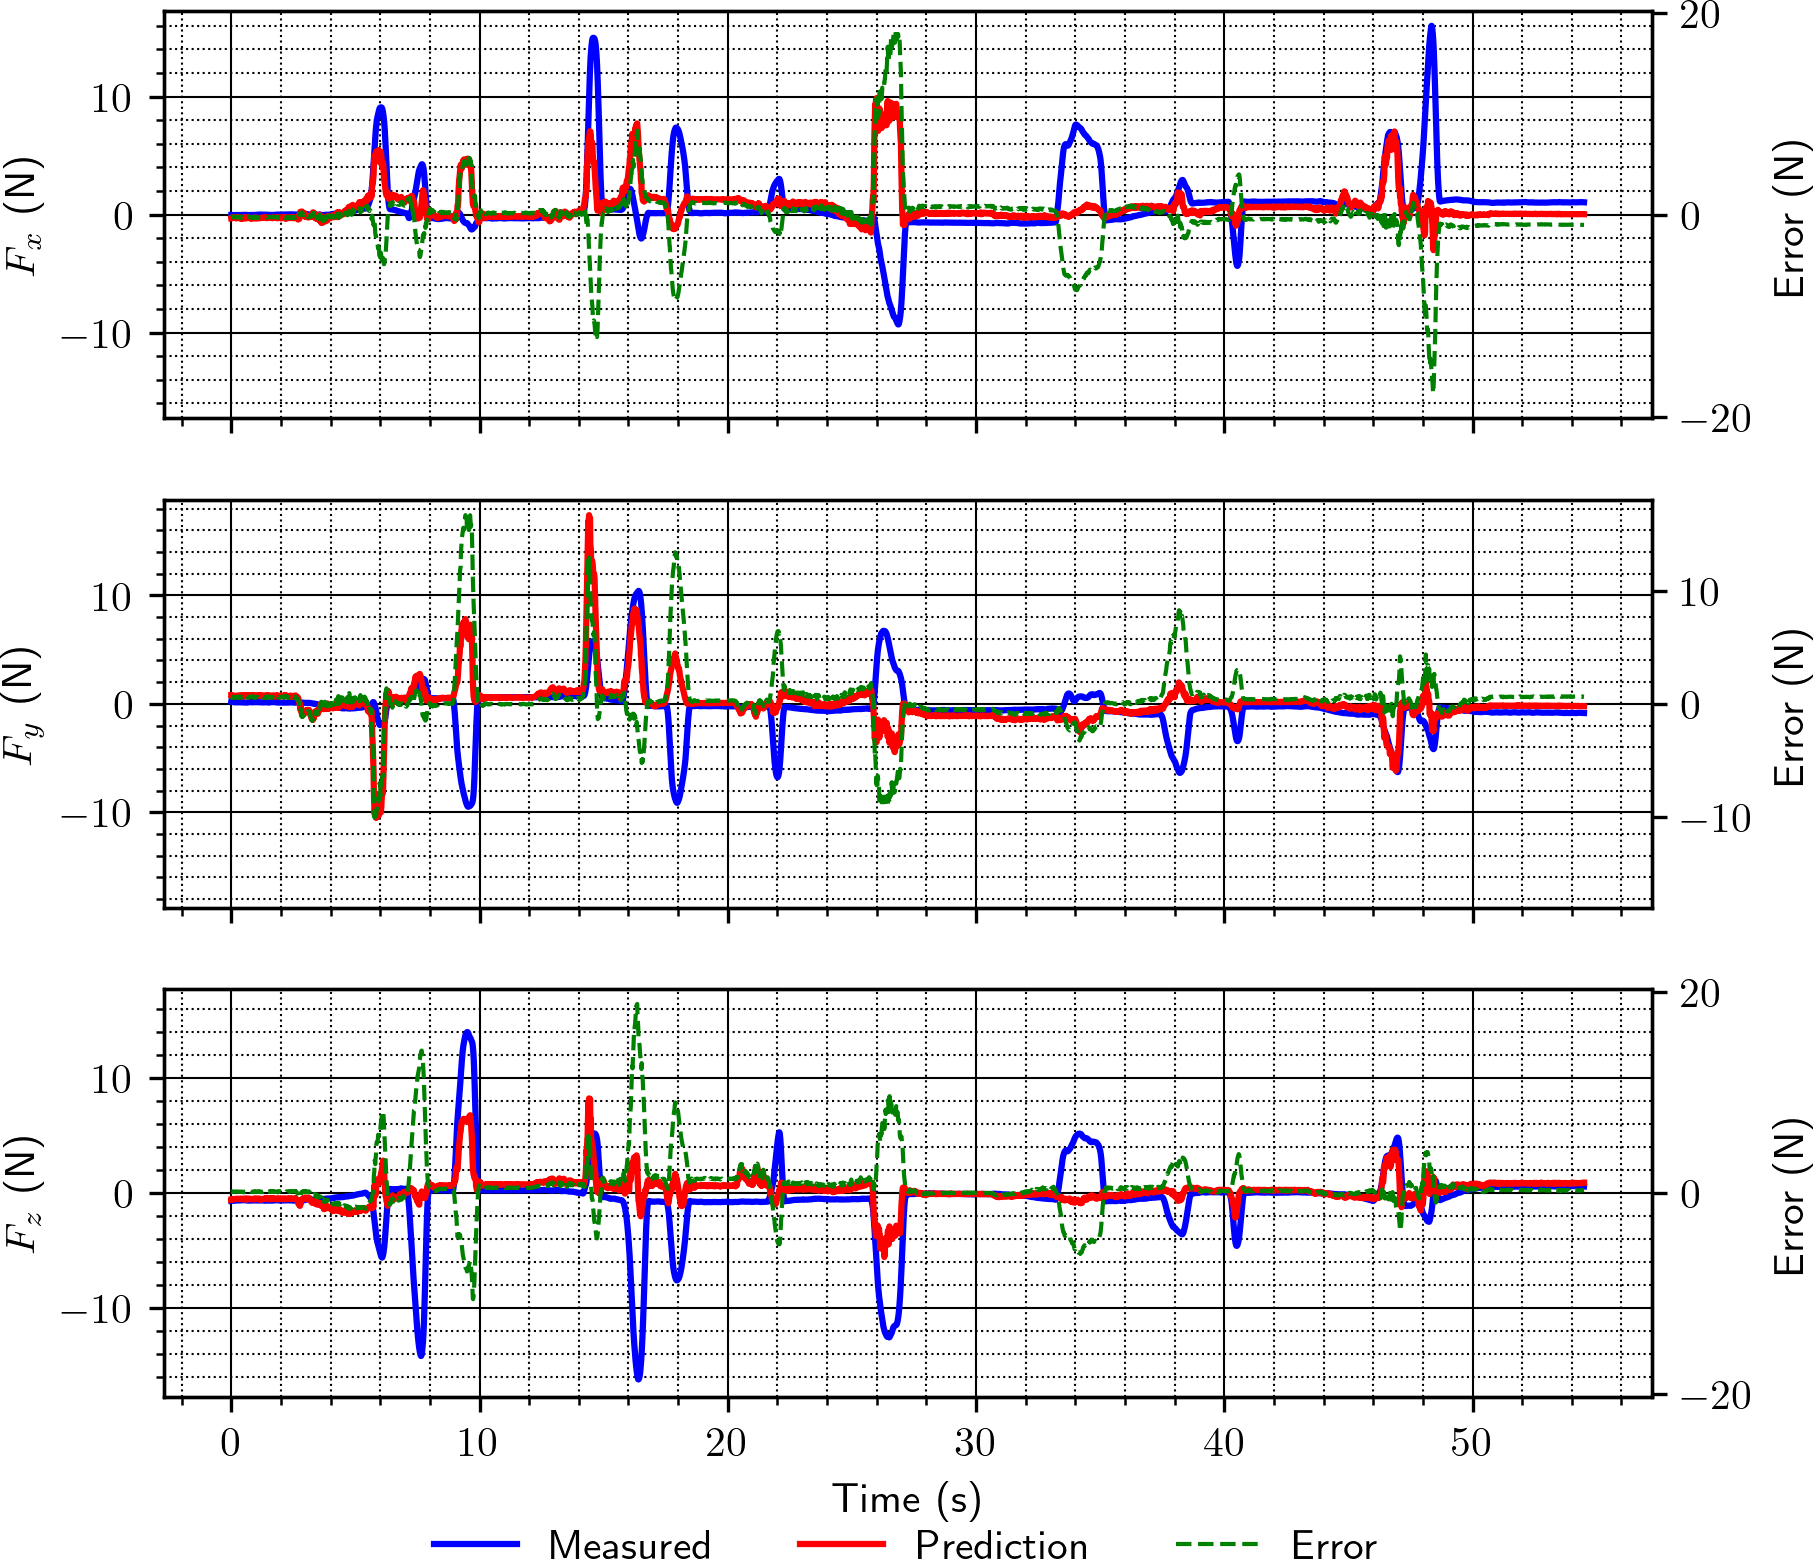
\includegraphics[width=0.48\columnwidth]{slike/Fig04_19b.png}}
    \vfil
    \subfloat[Convolutional (arch. \#6)]{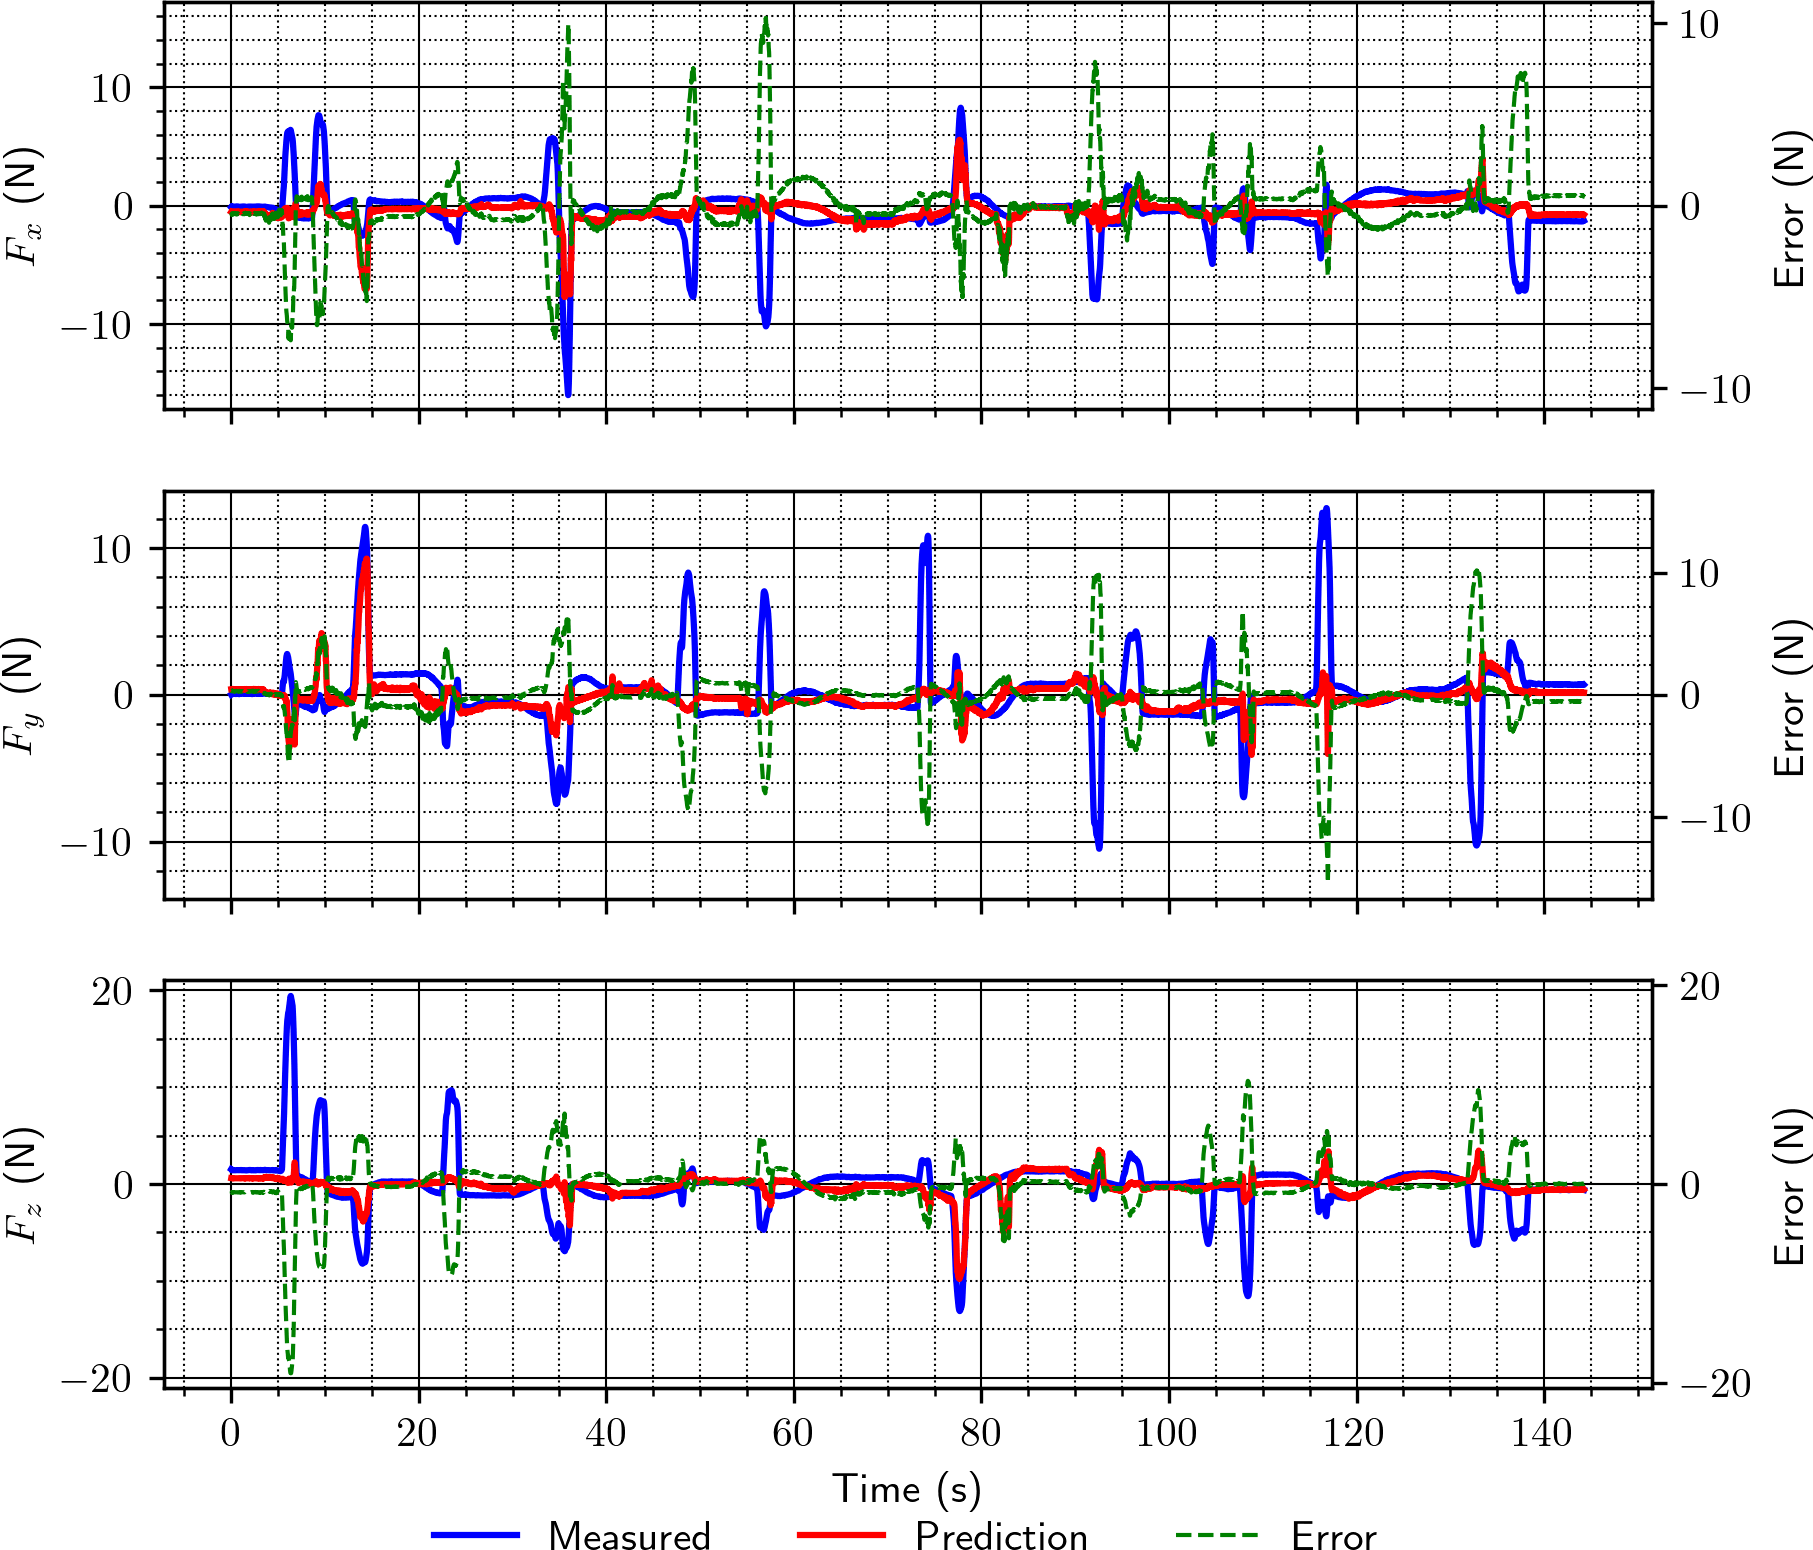
\includegraphics[width=0.48\columnwidth]{slike/Fig04_19c.png}}
    \hfil
    \subfloat[Convolutional (arch. \#4)]{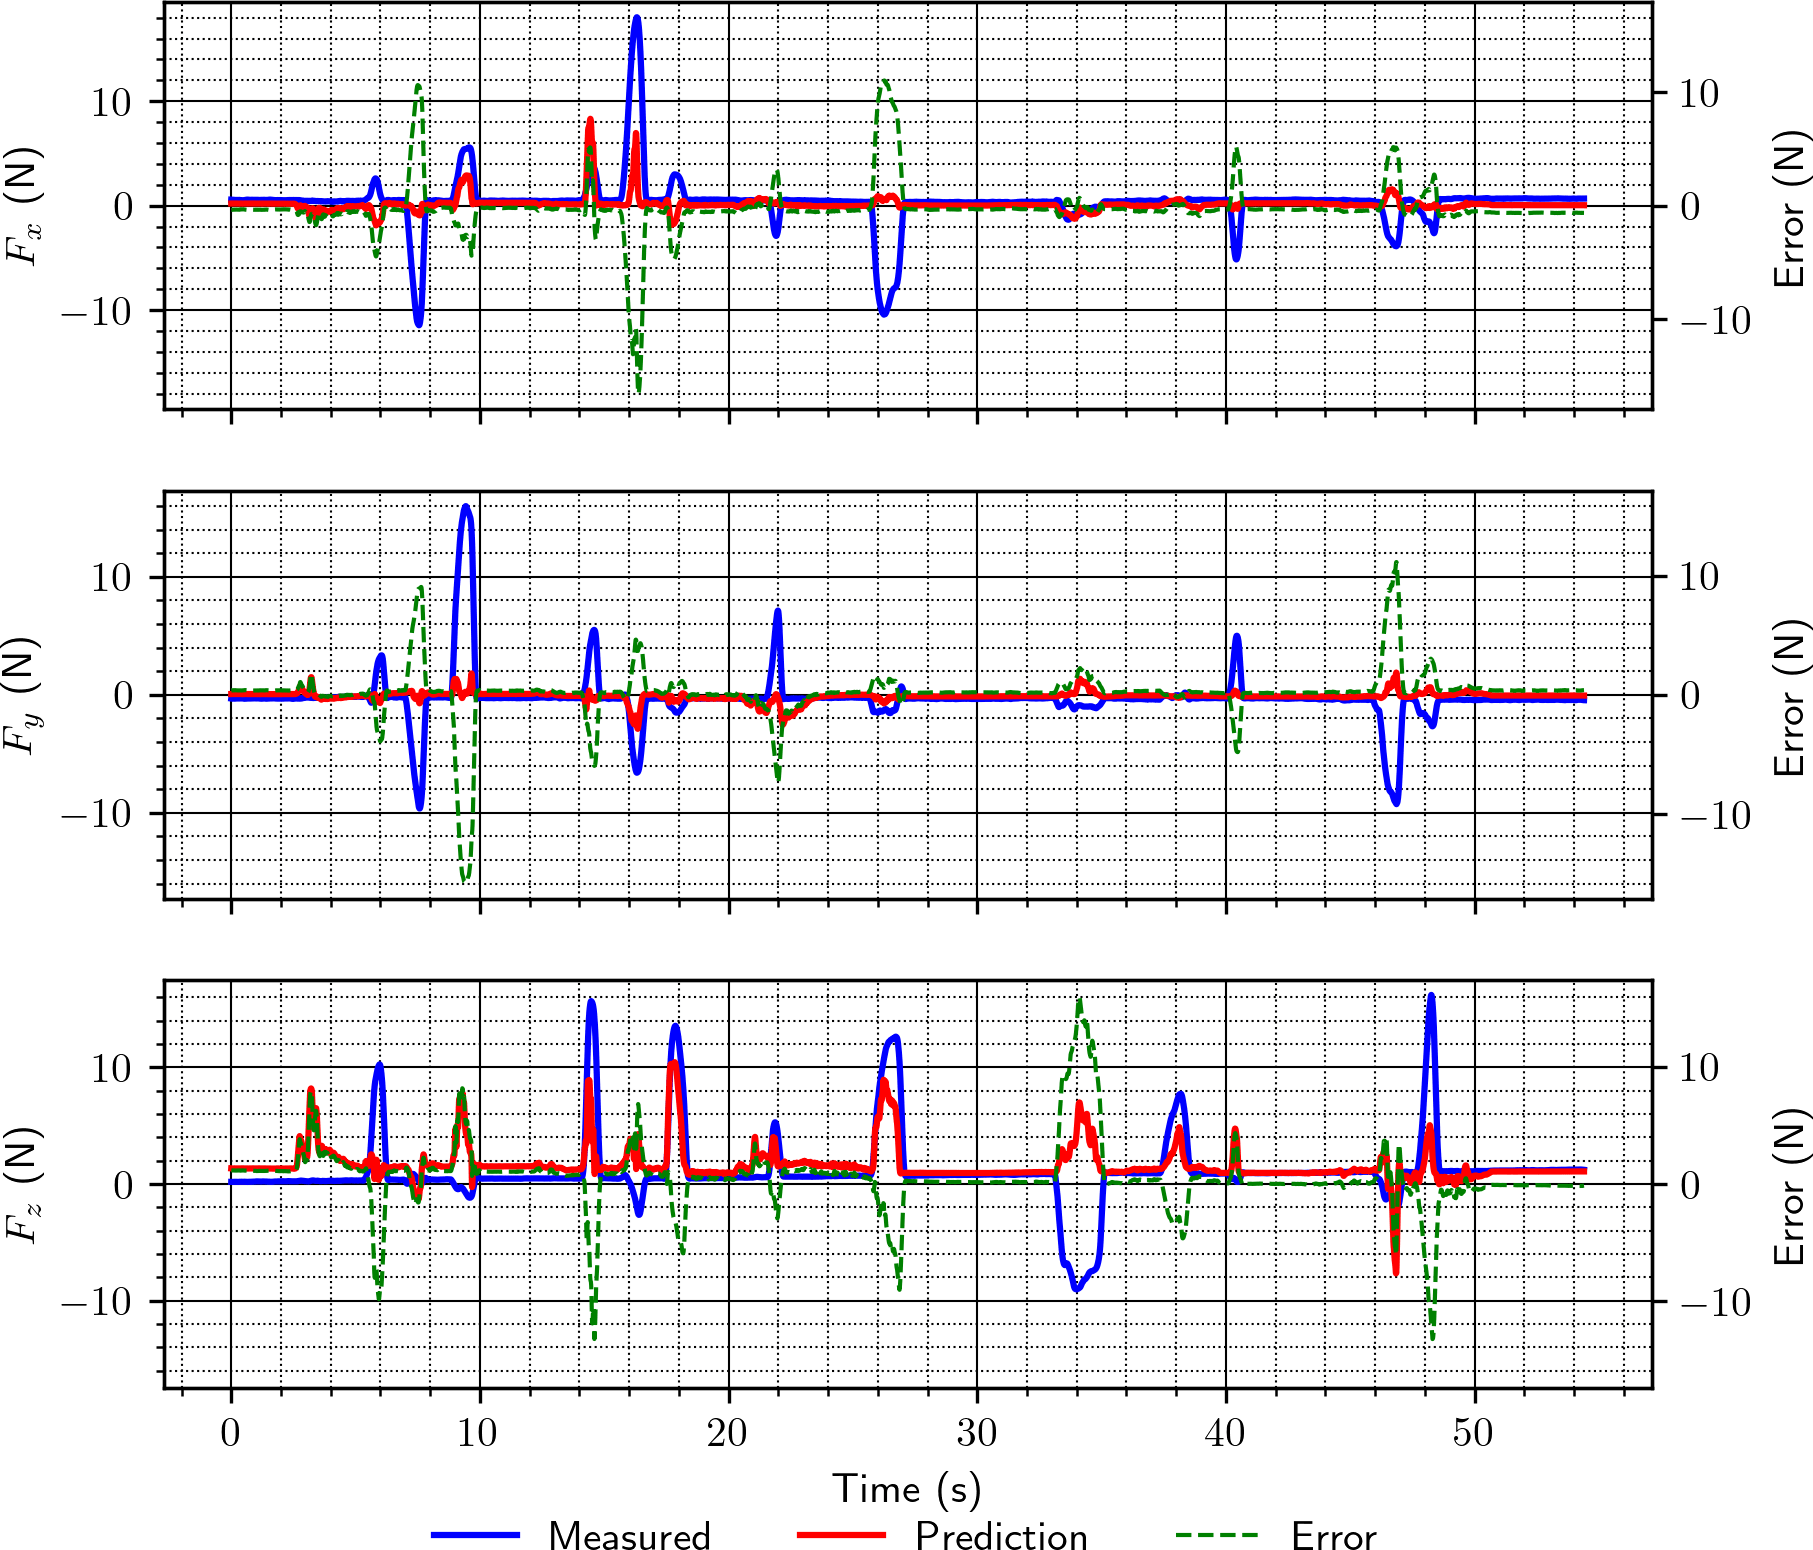
\includegraphics[width=0.48\columnwidth]{slike/Fig04_19d.png}}
    \vfil
    \subfloat[LSTM (arch. \#8)]{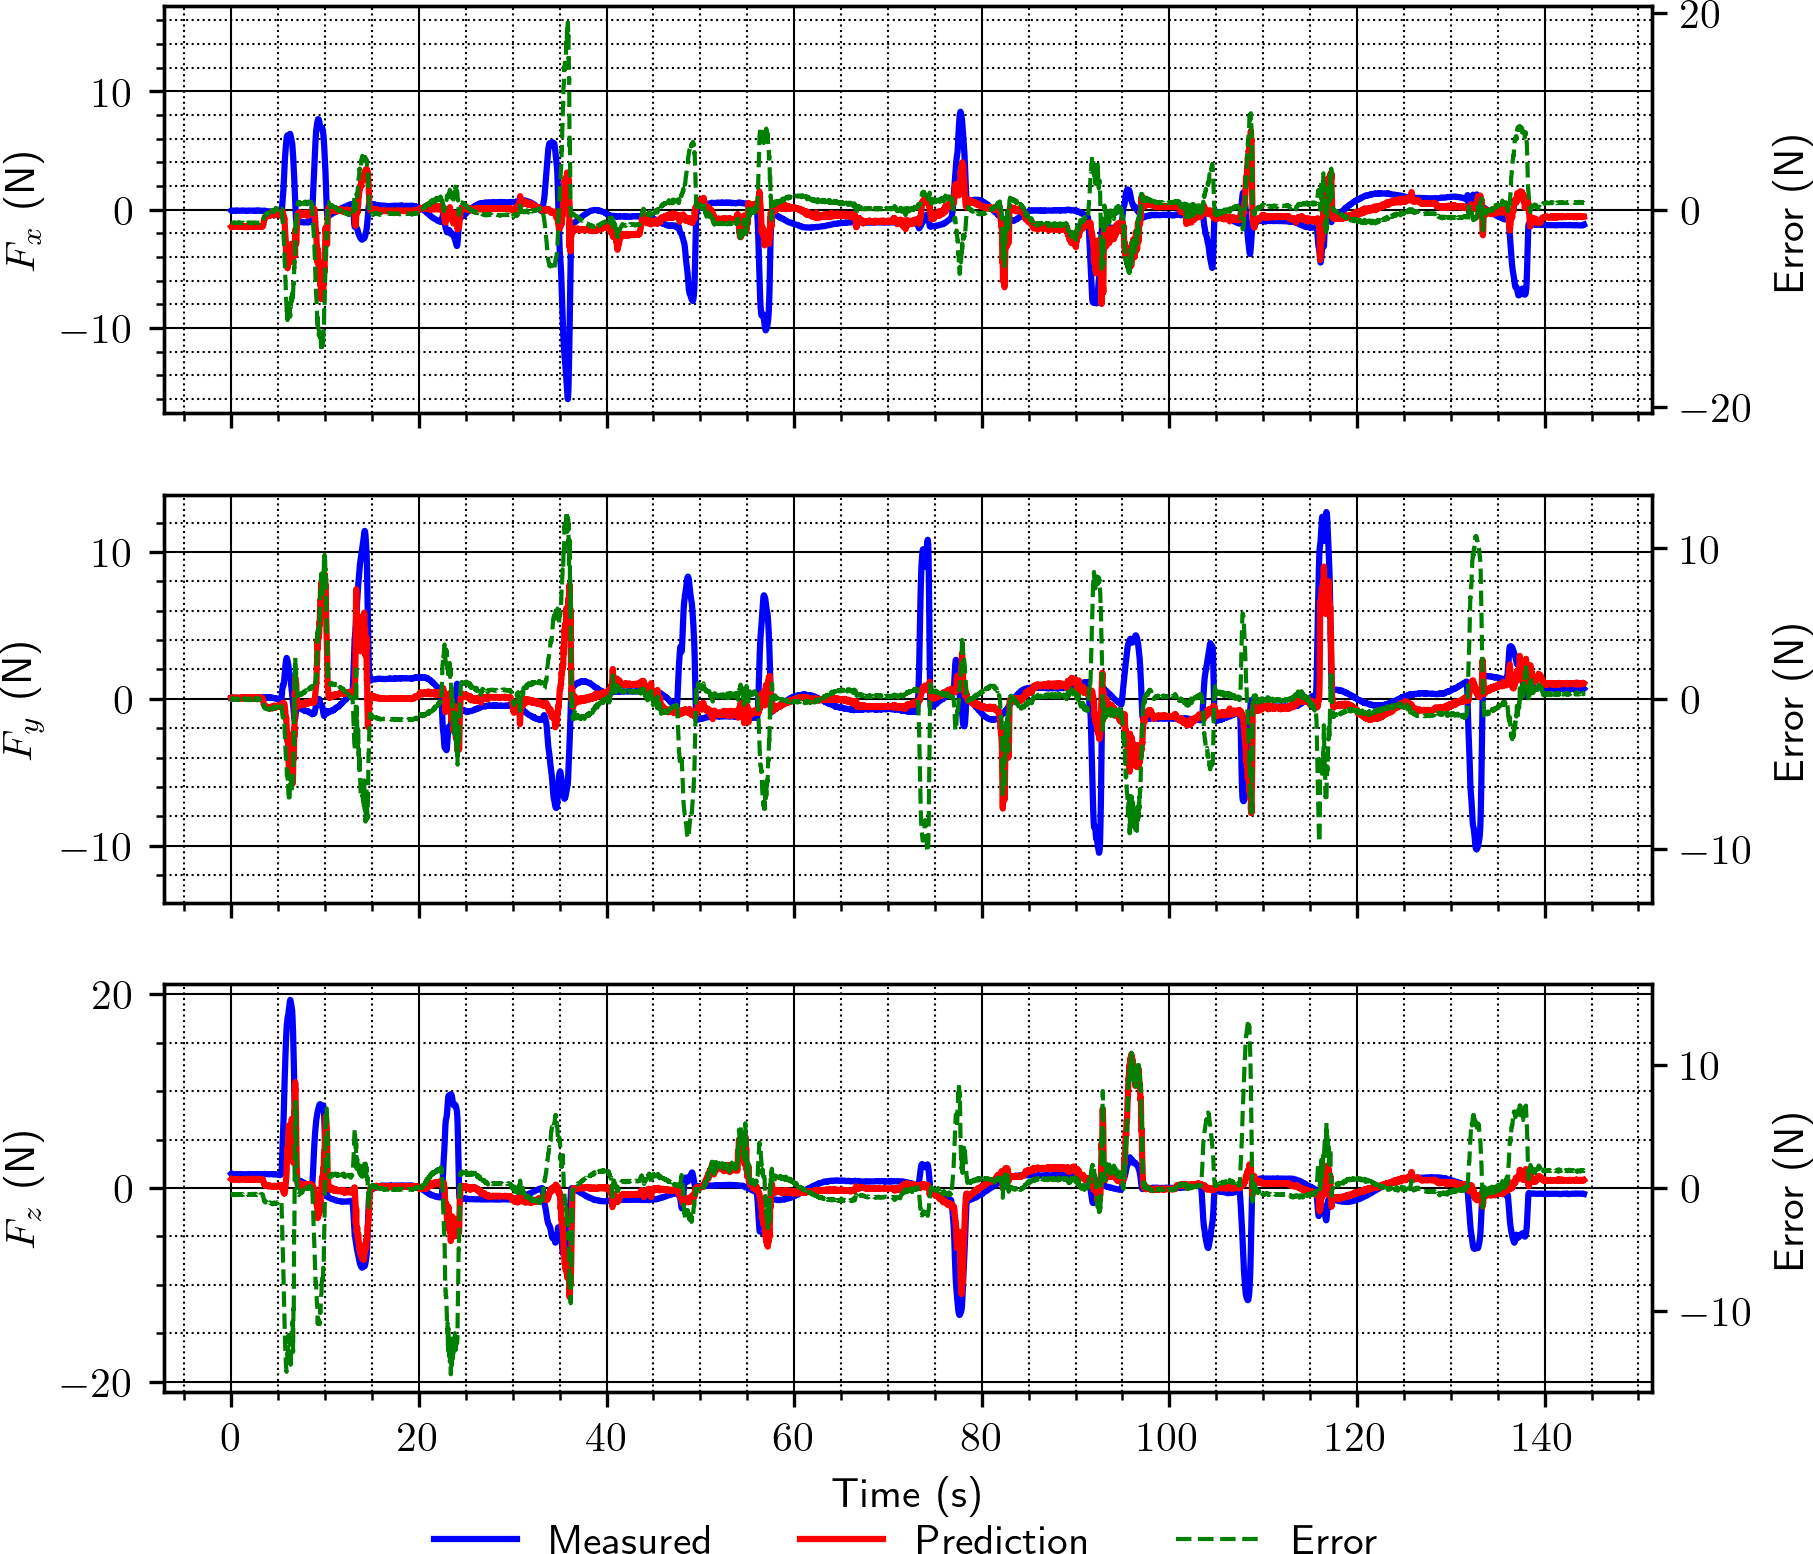
\includegraphics[width=0.48\columnwidth]{slike/Fig04_19e.png}}
    \hfil
    \subfloat[LTSM (arch. \#9)]{\includegraphics[width=0.48\columnwidth]{slike/Fig04_19f.png}}
    \caption{End-effector force prediction examples using real-world data for Franka robot}
    \label{fig:RealGraphs}
\end{figure}

After a thorough analysis, it was concluded that the result discrepancies are the flaw of the hardware and not of the presented method. Moreover, in support of this conclusion, it was proved that the method was adequately performing when using data obtained in simulation for the same robot, the same experimental setup, and the same data preprocessing procedure. Therefore, these discrepancies might likely be due to the time-varying drift in the force-torque sensor on the robot tip measurements. One more argument favouring this conclusion is that using the similar experimental setup for joint torques estimation, but without the sensor on the robot tip performed adequately, as reported in the following subsection.

\subsection{Joint torques estimation}
\label{sec:ResJoint}

The obtained results regarding joint torque estimation are reported and summarised in \cref{tab:NetworksFrankaTorqueRes}. Results obtained for the same experiment using simulation datasets are reported first, followed by the results obtained using real-world datasets.

\begin{table}
    \centering
    \caption{Trained neural networks for joint torques estimation}
    \label{tab:NetworksFrankaTorqueRes}
    \begin{tabular}{cccccc}
        \toprule
        \textbf{No.} & \textbf{Architecture} & \textbf{Dataset} & \textbf{Validation Loss} & \textbf{Test Loss} & \textbf{RMSE} \\
        \midrule
        1 & DeLaN & Sim (no ext.) & 0.6528 & 0.6826 & 0.5314 \\ % lnn_prazni_02
        2 & DeLaN & Sim (with ext.) & 1.2333 & 1.2137 & 0.7475 \\ % lnn_teret_02
        3 & MLP & Sim (with ext.) & 1.4070 & 1.4076 & 1.0287 \\ % mlp_tau_01
        4 & Conv & Sim (with ext.) & 1.1439 & 1.1420 & 0.9144 \\ % conv_teret_torque_01
        5 & LSTM & Sim (with ext.) & 0.6208 & 0.6236 & 0.6189\\ % lstm_teret_torque_01
        \midrule
        6 & DeLaN & Real & 1.3198 & 1.2398 & 0.8468\\ % lnn_franka_01
        7 & MLP & Real & 1.9336 & 1.8995 & 1.1567\\% mlp_franka_torque_01
        8 & Conv & Real & 1.4699 & 1.4837 & 0.9552\\ % conv_franka_torque_01
        9 & LSTM & Real & 1.1643 & 1.0385 & 0.7778\\ % lstm_franka_torque_01
        \midrule
        10 $^*$ & LSTM & Sim (with ext.) & 0.1236 & 0.1234 & \textbf{0.2974}\\ % optim_torque_02
        11 $^\dagger$ & LSTM & Real & 0.8989 & 0.9606 & \textbf{0.7369} \\ % optim_torque_franka_02
        \bottomrule
        \multicolumn{6}{l}{\footnotesize{$^*$ Optimised architecture: two LSTM layers (64 and 56 cells), and two FC layers (16 and 48 neurons)}}\\
        \multicolumn{6}{l}{\footnotesize{$^\dagger$ Optimised architecture: one LSTM layers (32 cells), and two FC layers (8 and 16 neurons)}}
    \end{tabular}
\end{table}

The torques were first estimated using DeLaN architecture, proposed in \cite{Lutter2019}. In that paper, the experiment that was conducted considered only four lower joints, since they ``dominate dynamics'' \cite{Lutter2019}. In our research, we trained the DeLaN network for all seven joints with the dataset that had no external forces acting and obtained reasonably good estimates, as shown in the two examples in \cref{fig:DeLaNRes}.

From the \cref{fig:DeLaNRes}, it is evident that the primary source of inconsistency between the actual and estimated torque plots/trajectories are joints 1 and 7. However, their relative contribution to the total error differs since they pertain to different torque scales as depicted by the y-axis ranges in the figure.

Predictions for joint 1 are inaccurate due to peaks in torque in the moments the robot starts or stops moving, which could not be learnt easily by this architecture. Besides the rare peaks during the whole measurement sequence, joint torques for this joint have small values, and thus it seems like the network is filtering out the peaks. On the other hand, with joint 7, estimates are inconsistent, but this may not be a critical issue since this joint contributes least to the whole robot dynamics. Also, similarly to joint 1, the torque values are minimal, compared to torques for other joints (i.e., other joint torques are at least one order of magnitude higher, often more).

When this architecture was trained on the dataset with external forces acting, the results were slightly worse: training and validation resulted in higher losses, and the estimates are not overlapping for the most part. The example is shown in \cref{fig:DeLaNResTeret}. The performance of this network is generally similar to the previous case, with observations about joints 1 and 7 holding. However, the estimates are somewhat less accurate with other joints than in the previous case. As it seems, when trained using a dataset with external forces, this network neglects external forces, i.e., the predictions are, as if there is no external force acting, which is especially visible in the estimates of joints 5 and 6, and on joint 4 to the lesser extent.

\begin{figure}
    \centering
    \subfloat[Example from dataset \emph{without} external forces\label{fig:DeLaNResEmpty}]{\includegraphics[width=0.48\textwidth]{slike/Fig04_20a.png}}
    \hfill
    \subfloat[Example from dataset \emph{with} external forces\label{fig:DeLaNResTeret}]{\includegraphics[width=0.48\textwidth]{slike/Fig04_20b.png}}
    \caption{Example torque estimates using DeLaN architecture with different datasets}
    \label{fig:DeLaNRes}
\end{figure}

Classical neural network architectures, especially LSTMs (which operate on sequences), perform well when external forces act on the robot, as shown in \cref{fig:ConvLSTMResTeret}. It turns out that their estimates are even better than DeLaN estimates (supported by RMSE values obtained on the test set, from \cref{tab:NetworksFrankaTorqueRes}), which leads to the conclusion that this architecture is well-suited for the task. However, some additional hyperparameter tuning may be needed to obtain even better results. Finally, the DeLaN network performs better when no external forces are acting (compared to when external forces are acting), a case that is not particularly useful for real applications but shows that this architecture captures the robot's dynamic model best (among ones tested).

\begin{figure}
    \centering
    \subfloat[Convolutional network]{\includegraphics[width=0.48\textwidth]{slike/Fig04_21a.png}}
    \hfill
    \subfloat[LSTM network]{\includegraphics[width=0.48\textwidth]{slike/Fig04_21b.png}}
    \caption{Example torque estimates using classical architectures with simulation dataset}
    \label{fig:ConvLSTMResTeret}
\end{figure}

The results obtained using data from the simulation are then compared to the ones from the real world. They are numerically (RMSE in the Table \ref{tab:NetworksFrankaTorqueRes}) and visually (\cref{fig:NetworksFrankaTorqueReal}) slightly worse than those from the simulation, but the same trends are followed. Thus, again, the LSTM network was identified as performing the best among the ones tested. 

In \cref{fig:NetworksFrankaTorqueReal}, the analytical model (obtained in \cite{Gaz2019}) was included for comparison. However, please note that the analytical model does not take external forces into account. Thus, the presented neural networks have better estimates than the analytical model when an external force is applied. The measured torques are mostly in line with analytical torques, except in some joints (mostly joints 4-6) and only in parts when the external force is applied. Torques for joint 1 from the analytical model look noisy (which is not the case with neural network predictions). In contrast, torques for joint 7, the analytical model, has shown better performance than predictions of any of the presented networks, but still not performing well, which should not be the issue since the amplitudes are small compared to the other joints outlined before in the discussion. 

It is essential to emphasise that the analytical model took almost three hours to compute the torques depicted in the figure, and the network evaluations took just about seconds. However, note that the analytical model was not optimised (a simple \emph{for} loop was used for the computations of each sample), and there is certainly possible that optimising it would take significantly less time to complete the calculations. However, it is expected that it will never outperform neural networks since the model is highly nonlinear.

\begin{figure}
    \centering
    \subfloat[DeLaN]{\includegraphics[width=0.47\textwidth]{slike/Fig04_22a.png}}
    \hfill
    \subfloat[MLP]{\includegraphics[width=0.47\textwidth]{slike/Fig04_22b.png}}
    \vfill
    \subfloat[Convolutional network]{\includegraphics[width=0.47\textwidth]{slike/Fig04_22c.png}}
    \hfill
    \subfloat[LSTM network]{\includegraphics[width=0.47\textwidth]{slike/Fig04_22d.png}}
    \caption{Torque estimates on the real-world dataset compared with the analytical model}
    \label{fig:NetworksFrankaTorqueReal}
\end{figure}

These results again emphasise that the error in results obtained in the experiment on end-effector force estimation with real-world dataset are likely due to incorrect readings of the tip-mounted force sensor.

In the case of joint torques estimation, hyperparameter optimisation was also performed using simulation and real-world datasets. Networks identified as best (among those considered during the optimisation process) had two LSTM layers with 64 and 56 cells, respectively, and two fully-connected layers with 16 and 48 neurons, respectively and ReLU activation function (for simulation dataset), and 1 LSTM layer with 32 cells and two fully-connected layers with 8 and 16 neurons (for real-world dataset). The simulation network performed significantly better than networks that were not optimised. This is especially evident in \cref{fig:JointTorqueOptim}, where significant improvements in the estimates for joints 1, 5, and 6 can be seen. Joint 1 peak predictions are now primarily correct, and joints 5 and 6 follow the measured values, thus reducing the error. The real-world optimised network performed only slightly better, and therefore RMSE is just marginally better than RMSE of the best network without optimisation.

\begin{figure}
    \centering
    \subfloat[In simulation]{\includegraphics[width=0.48\textwidth]{slike/Fig04_23a.png}}
    \hfill
    \subfloat[In real world]{\includegraphics[width=0.48\textwidth]{slike/Fig04_23b.png}}
    \caption{Example joint torque estimates for optimised LSTM network}
    \label{fig:JointTorqueOptim}
\end{figure}

If the proposed approach is to be applied in the real-world setting, especially for human-robot (force-based) interaction, the safety of the approach needs to be discussed (although not in the focus of this research). Assuming that the network was trained appropriately (with a sufficient amount and variety of data), additional potential sources of network malfunction (in terms of safety) could be faulty sensor readings and adversarial attacks on the network. Faulty sensor issues could be addressed by one of the fault diagnosis algorithms \cite{Li2020} (which include neural networks) before the data is fed to our network. Please note that this issue is present in all force measurement and estimation approaches regardless of which algorithm is being used. Adversarial attacks on convolutional networks are well documented, and known \cite{Heaven2019}, but these types of attacks are becoming more and more present in recurrent-type networks, including LSTM. Fortunately, countermeasures do exist \cite{Rosenberg2019} and could be deployed in real-world scenarios.

In the final experiment on joint torques estimation, an array of strain gauge force sensors was used to replace the expensive (but reliable) 3-axis force-torque sensor. The goal was to assess if using multiple low-cost single axis-sensors can obtain comparable results to those obtained with a 3-axis force sensor. 

The obtained results in the experiment are presented in \cref{tab:NetworksFrankaTorqueSG} and example estimates are shown in \cref{fig:NetworksFrankaSG}. 

\begin{table}
    \centering
    \caption{Trained neural networks for joint torques estimation using strain gauges}
    \label{tab:NetworksFrankaTorqueSG}
    \begin{tabular}{cccccc}
        \toprule
        \textbf{\#} & \textbf{Architecture} & \textbf{Dataset} & \textbf{Validation Loss} & \textbf{Test Loss} & \textbf{RMSE} \\
        \midrule
        1. & MLP & Real & 1.4801 & 1.4113 & 1.0704\\% mlp_sg_02
        2. & Conv & Real & 1.8613 & 1.7227 & 1.2055\\ % conv_sg_01
        3. & LSTM & Real & 1.0927 & 0.9969 &\textbf{0.8931}\\ % lstm_sg_01
        \bottomrule
    \end{tabular}
\end{table}

The obtained RMSE values show that the LSTM network performs best among those tested, in line with previous results obtained with the force-torque sensor. However, they are slightly worse, especially for joints 5 and 6, while joints 2--4 match almost perfectly, as shown in \ref{fig:NetworksFrankaSG}. However, including additional training data may improve the performance since the used dataset was not as diverse as the one used in the previous experiment. Nevertheless, these results demonstrate that the assumption about using an array of single-axis sensors is valid and can be used for the task. 

One thing noted in this experiment is that, surprisingly, this time, multilayer perceptron outperformed convolutional network, which never happened in the previous experiments. However, this can easily be due to the small training dataset that lacks diversity. Therefore, these results may change if the additional training data is included in the dataset.

\begin{figure}
    \centering
    \subfloat[MLP network]{\includegraphics[width=0.45\textwidth]{slike/Fig04_24a.png}}
    \hfill
    \subfloat[Convolutional network]{\includegraphics[width=0.45\textwidth]{slike/Fig04_24b.png}}
    \vfill
    \subfloat[LSTM network]{\includegraphics[width=0.45\textwidth]{slike/Fig04_24c.png}}
    \caption{Example torque estimates on the real-world dataset using an array of single-axis force sensors}
    \label{fig:NetworksFrankaSG}
\end{figure}

\newpage